\documentclass[twoside]{book}

% Packages required by doxygen
\usepackage{fixltx2e}
\usepackage{calc}
\usepackage{doxygen}
\usepackage[export]{adjustbox} % also loads graphicx
\usepackage{graphicx}
\usepackage[utf8]{inputenc}
\usepackage{makeidx}
\usepackage{multicol}
\usepackage{multirow}
\PassOptionsToPackage{warn}{textcomp}
\usepackage{textcomp}
\usepackage[nointegrals]{wasysym}
\usepackage[table]{xcolor}

% Font selection
\usepackage[T1]{fontenc}
\usepackage[scaled=.90]{helvet}
\usepackage{courier}
\usepackage{amssymb}
\usepackage{sectsty}
\renewcommand{\familydefault}{\sfdefault}
\allsectionsfont{%
  \fontseries{bc}\selectfont%
  \color{darkgray}%
}
\renewcommand{\DoxyLabelFont}{%
  \fontseries{bc}\selectfont%
  \color{darkgray}%
}
\newcommand{\+}{\discretionary{\mbox{\scriptsize$\hookleftarrow$}}{}{}}

% Page & text layout
\usepackage{geometry}
\geometry{%
  a4paper,%
  top=2.5cm,%
  bottom=2.5cm,%
  left=2.5cm,%
  right=2.5cm%
}
\tolerance=750
\hfuzz=15pt
\hbadness=750
\setlength{\emergencystretch}{15pt}
\setlength{\parindent}{0cm}
\setlength{\parskip}{3ex plus 2ex minus 2ex}
\makeatletter
\renewcommand{\paragraph}{%
  \@startsection{paragraph}{4}{0ex}{-1.0ex}{1.0ex}{%
    \normalfont\normalsize\bfseries\SS@parafont%
  }%
}
\renewcommand{\subparagraph}{%
  \@startsection{subparagraph}{5}{0ex}{-1.0ex}{1.0ex}{%
    \normalfont\normalsize\bfseries\SS@subparafont%
  }%
}
\makeatother

% Headers & footers
\usepackage{fancyhdr}
\pagestyle{fancyplain}
\fancyhead[LE]{\fancyplain{}{\bfseries\thepage}}
\fancyhead[CE]{\fancyplain{}{}}
\fancyhead[RE]{\fancyplain{}{\bfseries\leftmark}}
\fancyhead[LO]{\fancyplain{}{\bfseries\rightmark}}
\fancyhead[CO]{\fancyplain{}{}}
\fancyhead[RO]{\fancyplain{}{\bfseries\thepage}}
\fancyfoot[LE]{\fancyplain{}{}}
\fancyfoot[CE]{\fancyplain{}{}}
\fancyfoot[RE]{\fancyplain{}{\bfseries\scriptsize Generated by Doxygen }}
\fancyfoot[LO]{\fancyplain{}{\bfseries\scriptsize Generated by Doxygen }}
\fancyfoot[CO]{\fancyplain{}{}}
\fancyfoot[RO]{\fancyplain{}{}}
\renewcommand{\footrulewidth}{0.4pt}
\renewcommand{\chaptermark}[1]{%
  \markboth{#1}{}%
}
\renewcommand{\sectionmark}[1]{%
  \markright{\thesection\ #1}%
}

% Indices & bibliography
\usepackage{natbib}
\usepackage[titles]{tocloft}
\setcounter{tocdepth}{3}
\setcounter{secnumdepth}{5}
\makeindex

% Hyperlinks (required, but should be loaded last)
\usepackage{ifpdf}
\ifpdf
  \usepackage[pdftex,pagebackref=true]{hyperref}
\else
  \usepackage[ps2pdf,pagebackref=true]{hyperref}
\fi
\hypersetup{%
  colorlinks=true,%
  linkcolor=blue,%
  citecolor=blue,%
  unicode%
}

% Custom commands
\newcommand{\clearemptydoublepage}{%
  \newpage{\pagestyle{empty}\cleardoublepage}%
}

\usepackage{caption}
\captionsetup{labelsep=space,justification=centering,font={bf},singlelinecheck=off,skip=4pt,position=top}

%===== C O N T E N T S =====

\begin{document}

% Titlepage & ToC
\hypersetup{pageanchor=false,
             bookmarksnumbered=true,
             pdfencoding=unicode
            }
\pagenumbering{roman}
\begin{titlepage}
\vspace*{7cm}
\begin{center}%
{\Large Tram Netwerk }\\
\vspace*{1cm}
{\large Generated by Doxygen 1.8.11}\\
\end{center}
\end{titlepage}
\clearemptydoublepage
\tableofcontents
\clearemptydoublepage
\pagenumbering{arabic}
\hypersetup{pageanchor=true}

%--- Begin generated contents ---
\chapter{Metro Netwerk}
\label{index}\hypertarget{index}{}This is the documentation, created with Doxygen, for Project Software Engineering\+: Metro Network.

\subsection*{Usage }

There a 3 options for running the software\+:
\begin{DoxyEnumerate}
\item Entering the following command\+: ./\+Tram\+\_\+\+Netwerk This will use a hardcoded X\+ML File, defined in the main.\+cpp file.
\item Entering the following command\+: ./\+Tram\+\_\+\+Netwerk 1 $<$\+X\+M\+L$>$, in which $<$\+X\+M\+L$>$ is the relative path from the rootfolder to the X\+ML File
\item Entering the following command\+: ./\+Tram\+\_\+\+Netwerk 2 This will also use a hardcoded X\+ML File, defined in the main.\+cpp file, so two different files can be hardcoded for easy use.
\end{DoxyEnumerate}

To run the debug version of the executable, enter the following command\+: ./\+Tram\+\_\+\+Netwerk\+\_\+debug 
\chapter{Deprecated List}
\label{deprecated}
\hypertarget{deprecated}{}

\begin{DoxyRefList}
\item[\label{deprecated__deprecated000002}%
\hypertarget{deprecated__deprecated000002}{}%
Member \hyperlink{classTiXmlHandle_acb5fe8388a526289ea65e817a51e05e7}{Ti\+Xml\+Handle\+:\+:Element} () const ]use To\+Element. Return the handle as a \hyperlink{classTiXmlElement}{Ti\+Xml\+Element}. This may return null.  
\item[\label{deprecated__deprecated000001}%
\hypertarget{deprecated__deprecated000001}{}%
Member \hyperlink{classTiXmlHandle_ab44b723a8dc9af72838a303c079d0376}{Ti\+Xml\+Handle\+:\+:Node} () const ]use To\+Node. Return the handle as a \hyperlink{classTiXmlNode}{Ti\+Xml\+Node}. This may return null.  
\item[\label{deprecated__deprecated000003}%
\hypertarget{deprecated__deprecated000003}{}%
Member \hyperlink{classTiXmlHandle_a9fc739c8a18d160006f82572fc143d13}{Ti\+Xml\+Handle\+:\+:Text} () const ]use \hyperlink{classTiXmlHandle_a4ac53a652296203a5b5e13854d923586}{To\+Text()} Return the handle as a \hyperlink{classTiXmlText}{Ti\+Xml\+Text}. This may return null.  
\item[\label{deprecated__deprecated000004}%
\hypertarget{deprecated__deprecated000004}{}%
Member \hyperlink{classTiXmlHandle_a49675b74357ba2aae124657a9a1ef465}{Ti\+Xml\+Handle\+:\+:Unknown} () const ]use \hyperlink{classTiXmlHandle_a1381c17507a130767b1e23afc93b3674}{To\+Unknown()} Return the handle as a \hyperlink{classTiXmlUnknown}{Ti\+Xml\+Unknown}. This may return null. 
\end{DoxyRefList}
\chapter{Hierarchical Index}
\section{Class Hierarchy}
This inheritance list is sorted roughly, but not completely, alphabetically\+:\begin{DoxyCompactList}
\item \contentsline{section}{Parser}{\pageref{classParser}}{}
\item \contentsline{section}{Passagier}{\pageref{classPassagier}}{}
\item \contentsline{section}{Spoor}{\pageref{classSpoor}}{}
\item \contentsline{section}{Station}{\pageref{classStation}}{}
\item Station\begin{DoxyCompactList}
\item \contentsline{section}{Halte}{\pageref{classHalte}}{}
\item \contentsline{section}{Metrostation}{\pageref{classMetrostation}}{}
\end{DoxyCompactList}
\item \contentsline{section}{System}{\pageref{classSystem}}{}
\item \contentsline{section}{Ti\+Xml\+Attribute\+Set}{\pageref{classTiXmlAttributeSet}}{}
\item \contentsline{section}{Ti\+Xml\+Base}{\pageref{classTiXmlBase}}{}
\begin{DoxyCompactList}
\item \contentsline{section}{Ti\+Xml\+Attribute}{\pageref{classTiXmlAttribute}}{}
\item \contentsline{section}{Ti\+Xml\+Node}{\pageref{classTiXmlNode}}{}
\begin{DoxyCompactList}
\item \contentsline{section}{Ti\+Xml\+Comment}{\pageref{classTiXmlComment}}{}
\item \contentsline{section}{Ti\+Xml\+Declaration}{\pageref{classTiXmlDeclaration}}{}
\item \contentsline{section}{Ti\+Xml\+Document}{\pageref{classTiXmlDocument}}{}
\item \contentsline{section}{Ti\+Xml\+Element}{\pageref{classTiXmlElement}}{}
\item \contentsline{section}{Ti\+Xml\+Text}{\pageref{classTiXmlText}}{}
\item \contentsline{section}{Ti\+Xml\+Unknown}{\pageref{classTiXmlUnknown}}{}
\end{DoxyCompactList}
\end{DoxyCompactList}
\item \contentsline{section}{Ti\+Xml\+Cursor}{\pageref{structTiXmlCursor}}{}
\item \contentsline{section}{Ti\+Xml\+Handle}{\pageref{classTiXmlHandle}}{}
\item \contentsline{section}{Ti\+Xml\+Parsing\+Data}{\pageref{classTiXmlParsingData}}{}
\item \contentsline{section}{Ti\+Xml\+String}{\pageref{classTiXmlString}}{}
\begin{DoxyCompactList}
\item \contentsline{section}{Ti\+Xml\+Out\+Stream}{\pageref{classTiXmlOutStream}}{}
\end{DoxyCompactList}
\item \contentsline{section}{Ti\+Xml\+Visitor}{\pageref{classTiXmlVisitor}}{}
\begin{DoxyCompactList}
\item \contentsline{section}{Ti\+Xml\+Printer}{\pageref{classTiXmlPrinter}}{}
\end{DoxyCompactList}
\item \contentsline{section}{Tram}{\pageref{classTram}}{}
\item Tram\begin{DoxyCompactList}
\item \contentsline{section}{Albatros}{\pageref{classAlbatros}}{}
\item \contentsline{section}{P\+CC}{\pageref{classPCC}}{}
\end{DoxyCompactList}
\end{DoxyCompactList}

\chapter{Class Index}
\section{Class List}
Here are the classes, structs, unions and interfaces with brief descriptions\+:\begin{DoxyCompactList}
\item\contentsline{section}{\hyperlink{classStation}{Station} }{\pageref{classStation}}{}
\end{DoxyCompactList}

\chapter{File Index}
\section{File List}
Here is a list of all documented files with brief descriptions\+:\begin{DoxyCompactList}
\item\contentsline{section}{src/\+Parser/\hyperlink{Parser_8h}{Parser.\+h} \\*Header file for the \hyperlink{classParser}{Parser} Class }{\pageref{Parser_8h}}{}
\item\contentsline{section}{src/\+Passagier/\hyperlink{Passagier_8h}{Passagier.\+h} \\*Header file for the \hyperlink{classPassagier}{Passagier} Class }{\pageref{Passagier_8h}}{}
\item\contentsline{section}{src/\+Spoor/\hyperlink{Spoor_8h}{Spoor.\+h} \\*Header file for the \hyperlink{classSpoor}{Spoor} Class }{\pageref{Spoor_8h}}{}
\item\contentsline{section}{src/\+Station/\hyperlink{Halte_8h}{Halte.\+h} \\*Header file for the \hyperlink{classHalte}{Halte} Class }{\pageref{Halte_8h}}{}
\item\contentsline{section}{src/\+Station/\hyperlink{Metrostation_8h}{Metrostation.\+h} \\*Header file for the \hyperlink{classMetrostation}{Metrostation} Class }{\pageref{Metrostation_8h}}{}
\item\contentsline{section}{src/\+Station/\hyperlink{Station_8h}{Station.\+h} \\*Header file for the \hyperlink{classStation}{Station} Class }{\pageref{Station_8h}}{}
\item\contentsline{section}{src/\+System/\hyperlink{System_8h}{System.\+h} \\*Header file for \hyperlink{classSystem}{System} class }{\pageref{System_8h}}{}
\item\contentsline{section}{src/tinyxml/{\bfseries tinystr.\+h} }{\pageref{tinystr_8h}}{}
\item\contentsline{section}{src/tinyxml/{\bfseries tinyxml.\+h} }{\pageref{tinyxml_8h}}{}
\item\contentsline{section}{src/\+Tram/\hyperlink{Albatros_8h}{Albatros.\+h} \\*Header file for the \hyperlink{classAlbatros}{Albatros} Class }{\pageref{Albatros_8h}}{}
\item\contentsline{section}{src/\+Tram/{\bfseries P\+C\+C.\+h} }{\pageref{PCC_8h}}{}
\item\contentsline{section}{src/\+Tram/\hyperlink{Tram_8h}{Tram.\+h} \\*Header file for the \hyperlink{classPCC}{P\+CC} Class }{\pageref{Tram_8h}}{}
\end{DoxyCompactList}

\chapter{Class Documentation}
\hypertarget{classAlbatros}{}\section{Albatros Class Reference}
\label{classAlbatros}\index{Albatros@{Albatros}}


Inheritance diagram for Albatros\+:\nopagebreak
\begin{figure}[H]
\begin{center}
\leavevmode
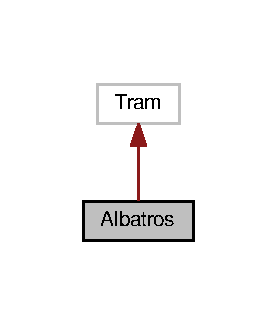
\includegraphics[width=133pt]{classAlbatros__inherit__graph}
\end{center}
\end{figure}


Collaboration diagram for Albatros\+:\nopagebreak
\begin{figure}[H]
\begin{center}
\leavevmode
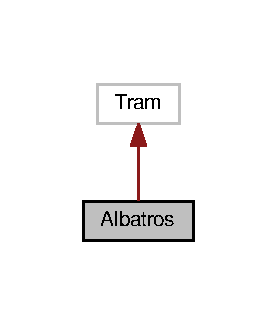
\includegraphics[width=133pt]{classAlbatros__coll__graph}
\end{center}
\end{figure}
\subsection*{Public Member Functions}
\begin{DoxyCompactItemize}
\item 
bool {\bfseries is\+Albatros} ()\hypertarget{classAlbatros_a899d40adaadbd53c0f99fd08a2c91cf7}{}\label{classAlbatros_a899d40adaadbd53c0f99fd08a2c91cf7}

\item 
string {\bfseries type\+String} ()\hypertarget{classAlbatros_ad1d8db48a50695b66117033911597513}{}\label{classAlbatros_ad1d8db48a50695b66117033911597513}

\end{DoxyCompactItemize}


The documentation for this class was generated from the following files\+:\begin{DoxyCompactItemize}
\item 
src/\+Tram/Albatros.\+h\item 
src/\+Tram/Albatros.\+cpp\end{DoxyCompactItemize}

\hypertarget{classHalte}{}\section{Halte Class Reference}
\label{classHalte}\index{Halte@{Halte}}


Inheritance diagram for Halte\+:\nopagebreak
\begin{figure}[H]
\begin{center}
\leavevmode
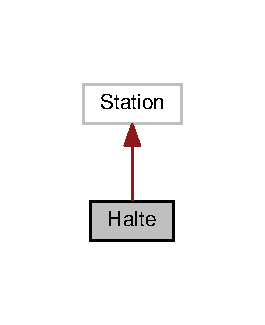
\includegraphics[width=127pt]{classHalte__inherit__graph}
\end{center}
\end{figure}


Collaboration diagram for Halte\+:\nopagebreak
\begin{figure}[H]
\begin{center}
\leavevmode
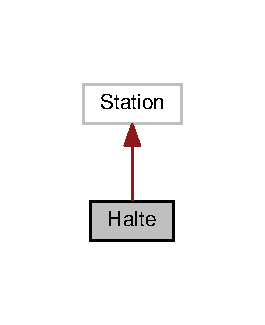
\includegraphics[width=127pt]{classHalte__coll__graph}
\end{center}
\end{figure}
\subsection*{Public Member Functions}
\begin{DoxyCompactItemize}
\item 
string {\bfseries type\+String} ()\hypertarget{classHalte_a8f1ba2d889f79a81d72d9c401732f8b6}{}\label{classHalte_a8f1ba2d889f79a81d72d9c401732f8b6}

\item 
bool {\bfseries is\+Metrostation} ()\hypertarget{classHalte_a292876fb9d440119c7f6dafe19913e2d}{}\label{classHalte_a292876fb9d440119c7f6dafe19913e2d}

\end{DoxyCompactItemize}


The documentation for this class was generated from the following files\+:\begin{DoxyCompactItemize}
\item 
src/\+Station/Halte.\+h\item 
src/\+Station/Halte.\+cpp\end{DoxyCompactItemize}

\hypertarget{classMetrostation}{}\section{Metrostation Class Reference}
\label{classMetrostation}\index{Metrostation@{Metrostation}}


Inheritance diagram for Metrostation\+:\nopagebreak
\begin{figure}[H]
\begin{center}
\leavevmode
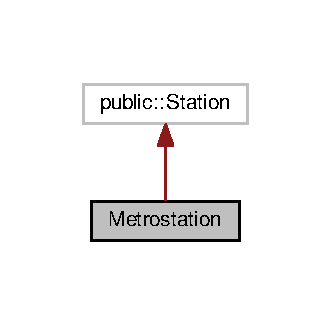
\includegraphics[width=159pt]{classMetrostation__inherit__graph}
\end{center}
\end{figure}


Collaboration diagram for Metrostation\+:\nopagebreak
\begin{figure}[H]
\begin{center}
\leavevmode
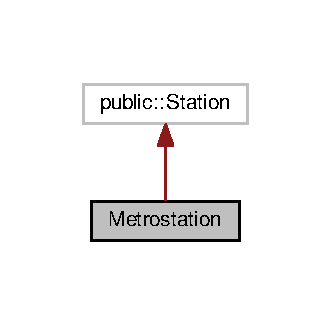
\includegraphics[width=159pt]{classMetrostation__coll__graph}
\end{center}
\end{figure}
\subsection*{Public Member Functions}
\begin{DoxyCompactItemize}
\item 
string {\bfseries type\+String} ()\hypertarget{classMetrostation_afc130023eefd0a8360358607b0d807d7}{}\label{classMetrostation_afc130023eefd0a8360358607b0d807d7}

\item 
bool {\bfseries is\+Metrostation} ()\hypertarget{classMetrostation_a5086b119e97721b2a82919f612788c4e}{}\label{classMetrostation_a5086b119e97721b2a82919f612788c4e}

\end{DoxyCompactItemize}


The documentation for this class was generated from the following files\+:\begin{DoxyCompactItemize}
\item 
src/\+Station/Metrostation.\+h\item 
src/\+Station/Metrostation.\+cpp\end{DoxyCompactItemize}

\hypertarget{classParser}{}\section{Parser Class Reference}
\label{classParser}\index{Parser@{Parser}}


This Class contains all the functionalities for the \hyperlink{classParser}{Parser} objects.  




{\ttfamily \#include $<$Parser.\+h$>$}

\subsection*{Public Member Functions}
\begin{DoxyCompactItemize}
\item 
\hyperlink{classParser_a12234f6cd36b61af4b50c94a179422c1}{Parser} ()\hypertarget{classParser_a12234f6cd36b61af4b50c94a179422c1}{}\label{classParser_a12234f6cd36b61af4b50c94a179422c1}

\begin{DoxyCompactList}\small\item\em \hyperlink{classParser}{Parser} Default Constructor. \end{DoxyCompactList}\item 
\hyperlink{classSystem}{System} $\ast$ \hyperlink{classParser_addad80574e43b744a82807d0f821d414}{get\+System} () const 
\begin{DoxyCompactList}\small\item\em Returns the \hyperlink{classParser}{Parser} object\textquotesingle{}s \hyperlink{classSystem}{System} Object. \end{DoxyCompactList}\item 
void {\bfseries set\+System} (\hyperlink{classSystem}{System} $\ast$system)\hypertarget{classParser_aaf58c6aafde4e7b889fbaa5d1f3aa6fe}{}\label{classParser_aaf58c6aafde4e7b889fbaa5d1f3aa6fe}

\item 
string \hyperlink{classParser_a36b746dbf631544851e0af2d0e7c6982}{get\+Element} (\hyperlink{classTiXmlElement}{Ti\+Xml\+Element} $\ast$elem)
\begin{DoxyCompactList}\small\item\em Returns the text contained in a \hyperlink{classTiXmlElement}{Ti\+Xml\+Element} Object. \end{DoxyCompactList}\item 
bool \hyperlink{classParser_aa8cdba8032e5d5d87b249be597b196c7}{Xml\+Parser} (string input\+File)
\begin{DoxyCompactList}\small\item\em Returns true if the inputfile is correctly parsed, false if not. \end{DoxyCompactList}\item 
bool \hyperlink{classParser_a8f97eab6905436595f33dc82b8957bbd}{is\+\_\+number} (string s)
\begin{DoxyCompactList}\small\item\em Returns true if the entered string is a number, false if not. \end{DoxyCompactList}\end{DoxyCompactItemize}


\subsection{Detailed Description}
This Class contains all the functionalities for the \hyperlink{classParser}{Parser} objects. 

\begin{DoxyAuthor}{Authors}
Loreas Clonen \& Luuk van Sloun 
\end{DoxyAuthor}


\subsection{Member Function Documentation}
\index{Parser@{Parser}!get\+Element@{get\+Element}}
\index{get\+Element@{get\+Element}!Parser@{Parser}}
\subsubsection[{\texorpdfstring{get\+Element(\+Ti\+Xml\+Element $\ast$elem)}{getElement(TiXmlElement *elem)}}]{\setlength{\rightskip}{0pt plus 5cm}string Parser\+::get\+Element (
\begin{DoxyParamCaption}
\item[{{\bf Ti\+Xml\+Element} $\ast$}]{elem}
\end{DoxyParamCaption}
)}\hypertarget{classParser_a36b746dbf631544851e0af2d0e7c6982}{}\label{classParser_a36b746dbf631544851e0af2d0e7c6982}


Returns the text contained in a \hyperlink{classTiXmlElement}{Ti\+Xml\+Element} Object. 

\begin{DoxyReturn}{Returns}
string 
\end{DoxyReturn}
\index{Parser@{Parser}!get\+System@{get\+System}}
\index{get\+System@{get\+System}!Parser@{Parser}}
\subsubsection[{\texorpdfstring{get\+System() const }{getSystem() const }}]{\setlength{\rightskip}{0pt plus 5cm}{\bf System} $\ast$ Parser\+::get\+System (
\begin{DoxyParamCaption}
{}
\end{DoxyParamCaption}
) const}\hypertarget{classParser_addad80574e43b744a82807d0f821d414}{}\label{classParser_addad80574e43b744a82807d0f821d414}


Returns the \hyperlink{classParser}{Parser} object\textquotesingle{}s \hyperlink{classSystem}{System} Object. 

Sets a new \hyperlink{classParser}{Parser} object\textquotesingle{}s \hyperlink{classSystem}{System} Object.

\begin{DoxyReturn}{Returns}
\hyperlink{classSystem}{System} Pointer
\end{DoxyReturn}

\begin{DoxyParams}{Parameters}
{\em system} & -\/ \hyperlink{classSystem}{System} Pointer \\
\hline
\end{DoxyParams}
\index{Parser@{Parser}!is\+\_\+number@{is\+\_\+number}}
\index{is\+\_\+number@{is\+\_\+number}!Parser@{Parser}}
\subsubsection[{\texorpdfstring{is\+\_\+number(string s)}{is_number(string s)}}]{\setlength{\rightskip}{0pt plus 5cm}bool Parser\+::is\+\_\+number (
\begin{DoxyParamCaption}
\item[{string}]{s}
\end{DoxyParamCaption}
)}\hypertarget{classParser_a8f97eab6905436595f33dc82b8957bbd}{}\label{classParser_a8f97eab6905436595f33dc82b8957bbd}


Returns true if the entered string is a number, false if not. 

\begin{DoxyReturn}{Returns}
boolean 
\end{DoxyReturn}
\index{Parser@{Parser}!Xml\+Parser@{Xml\+Parser}}
\index{Xml\+Parser@{Xml\+Parser}!Parser@{Parser}}
\subsubsection[{\texorpdfstring{Xml\+Parser(string input\+File)}{XmlParser(string inputFile)}}]{\setlength{\rightskip}{0pt plus 5cm}bool Parser\+::\+Xml\+Parser (
\begin{DoxyParamCaption}
\item[{string}]{input\+File}
\end{DoxyParamCaption}
)}\hypertarget{classParser_aa8cdba8032e5d5d87b249be597b196c7}{}\label{classParser_aa8cdba8032e5d5d87b249be597b196c7}


Returns true if the inputfile is correctly parsed, false if not. 

\begin{DoxyReturn}{Returns}
boolean 
\end{DoxyReturn}


The documentation for this class was generated from the following files\+:\begin{DoxyCompactItemize}
\item 
src/\+Parser/\hyperlink{Parser_8h}{Parser.\+h}\item 
src/\+Parser/Parser.\+cpp\end{DoxyCompactItemize}

\hypertarget{classPassagier}{}\section{Passagier Class Reference}
\label{classPassagier}\index{Passagier@{Passagier}}


This Class contains all the functionalities for the \hyperlink{classPassagier}{Passagier} objects.  




{\ttfamily \#include $<$Passagier.\+h$>$}

\subsection*{Public Member Functions}
\begin{DoxyCompactItemize}
\item 
\hyperlink{classPassagier_a1a2bc82f5780448cd2a9a47d08cc824f}{Passagier} ()\hypertarget{classPassagier_a1a2bc82f5780448cd2a9a47d08cc824f}{}\label{classPassagier_a1a2bc82f5780448cd2a9a47d08cc824f}

\begin{DoxyCompactList}\small\item\em Passenger Default Constructor. \end{DoxyCompactList}\item 
bool \hyperlink{classPassagier_ae271ce7875b2a7d17704e204ce9d8568}{properly\+Initialized} ()
\begin{DoxyCompactList}\small\item\em Returns true if properly initialized, false if not. \end{DoxyCompactList}\item 
string \hyperlink{classPassagier_aa9a9b53d417979551b0cb30fb0fdd232}{get\+Naam} ()
\begin{DoxyCompactList}\small\item\em Returns the \hyperlink{classStation}{Station} object\textquotesingle{}s name. \end{DoxyCompactList}\item 
void \hyperlink{classPassagier_a8d7a04358b35de18f378d048610e9aff}{set\+Naam} (string naam)
\begin{DoxyCompactList}\small\item\em Sets a new Passenger object\textquotesingle{}s name. \end{DoxyCompactList}\item 
string \hyperlink{classPassagier_a41e0870bb942364181aa17e2c9c7ca6c}{get\+Begin\+Station} ()
\begin{DoxyCompactList}\small\item\em Returns the Passenger object\textquotesingle{}s Starting \hyperlink{classStation}{Station}. \end{DoxyCompactList}\item 
void \hyperlink{classPassagier_afc4826ff4dacbbe15f15f6e8ef338ff0}{set\+Begin\+Station} (string begin\+Station)
\begin{DoxyCompactList}\small\item\em Sets a new Passenger object\textquotesingle{}s Starting \hyperlink{classStation}{Station}. \end{DoxyCompactList}\item 
string \hyperlink{classPassagier_a721949463e02e122567c9967786a8a38}{get\+Eind\+Station} ()
\begin{DoxyCompactList}\small\item\em Returns the Passenger object\textquotesingle{}s End \hyperlink{classStation}{Station}. \end{DoxyCompactList}\item 
void \hyperlink{classPassagier_a93606f0982849fc1838b5e16ab5f1b12}{set\+Eind\+Station} (string eind\+Station)
\begin{DoxyCompactList}\small\item\em Sets a new Passenger object\textquotesingle{}s End \hyperlink{classStation}{Station}. \end{DoxyCompactList}\item 
int \hyperlink{classPassagier_a1fd825eaa3db5b68cc24ca297e45d198}{get\+Hoeveelheid} ()
\begin{DoxyCompactList}\small\item\em Returns the Passenger object\textquotesingle{}s amount. \end{DoxyCompactList}\item 
void \hyperlink{classPassagier_adf498b0e24ef821f30e479591da7a3d3}{set\+Hoeveelheid} (int hoeveelheid)
\begin{DoxyCompactList}\small\item\em Sets a new Passenger object\textquotesingle{}s amount. \end{DoxyCompactList}\end{DoxyCompactItemize}


\subsection{Detailed Description}
This Class contains all the functionalities for the \hyperlink{classPassagier}{Passagier} objects. 

\begin{DoxyAuthor}{Authors}
Loreas Clonen \& Luuk van Sloun 
\end{DoxyAuthor}


\subsection{Member Function Documentation}
\index{Passagier@{Passagier}!get\+Begin\+Station@{get\+Begin\+Station}}
\index{get\+Begin\+Station@{get\+Begin\+Station}!Passagier@{Passagier}}
\subsubsection[{\texorpdfstring{get\+Begin\+Station()}{getBeginStation()}}]{\setlength{\rightskip}{0pt plus 5cm}string Passagier\+::get\+Begin\+Station (
\begin{DoxyParamCaption}
{}
\end{DoxyParamCaption}
)}\hypertarget{classPassagier_a41e0870bb942364181aa17e2c9c7ca6c}{}\label{classPassagier_a41e0870bb942364181aa17e2c9c7ca6c}


Returns the Passenger object\textquotesingle{}s Starting \hyperlink{classStation}{Station}. 

\begin{DoxyReturn}{Returns}
string 
\end{DoxyReturn}
\index{Passagier@{Passagier}!get\+Eind\+Station@{get\+Eind\+Station}}
\index{get\+Eind\+Station@{get\+Eind\+Station}!Passagier@{Passagier}}
\subsubsection[{\texorpdfstring{get\+Eind\+Station()}{getEindStation()}}]{\setlength{\rightskip}{0pt plus 5cm}string Passagier\+::get\+Eind\+Station (
\begin{DoxyParamCaption}
{}
\end{DoxyParamCaption}
)}\hypertarget{classPassagier_a721949463e02e122567c9967786a8a38}{}\label{classPassagier_a721949463e02e122567c9967786a8a38}


Returns the Passenger object\textquotesingle{}s End \hyperlink{classStation}{Station}. 

\begin{DoxyReturn}{Returns}
string 
\end{DoxyReturn}
\index{Passagier@{Passagier}!get\+Hoeveelheid@{get\+Hoeveelheid}}
\index{get\+Hoeveelheid@{get\+Hoeveelheid}!Passagier@{Passagier}}
\subsubsection[{\texorpdfstring{get\+Hoeveelheid()}{getHoeveelheid()}}]{\setlength{\rightskip}{0pt plus 5cm}string Passagier\+::get\+Hoeveelheid (
\begin{DoxyParamCaption}
{}
\end{DoxyParamCaption}
)}\hypertarget{classPassagier_a1fd825eaa3db5b68cc24ca297e45d198}{}\label{classPassagier_a1fd825eaa3db5b68cc24ca297e45d198}


Returns the Passenger object\textquotesingle{}s amount. 

\begin{DoxyReturn}{Returns}
integer 
\end{DoxyReturn}
\index{Passagier@{Passagier}!get\+Naam@{get\+Naam}}
\index{get\+Naam@{get\+Naam}!Passagier@{Passagier}}
\subsubsection[{\texorpdfstring{get\+Naam()}{getNaam()}}]{\setlength{\rightskip}{0pt plus 5cm}string Passagier\+::get\+Naam (
\begin{DoxyParamCaption}
{}
\end{DoxyParamCaption}
)}\hypertarget{classPassagier_aa9a9b53d417979551b0cb30fb0fdd232}{}\label{classPassagier_aa9a9b53d417979551b0cb30fb0fdd232}


Returns the \hyperlink{classStation}{Station} object\textquotesingle{}s name. 

\begin{DoxyReturn}{Returns}
string 
\end{DoxyReturn}
\index{Passagier@{Passagier}!properly\+Initialized@{properly\+Initialized}}
\index{properly\+Initialized@{properly\+Initialized}!Passagier@{Passagier}}
\subsubsection[{\texorpdfstring{properly\+Initialized()}{properlyInitialized()}}]{\setlength{\rightskip}{0pt plus 5cm}bool Passagier\+::properly\+Initialized (
\begin{DoxyParamCaption}
{}
\end{DoxyParamCaption}
)}\hypertarget{classPassagier_ae271ce7875b2a7d17704e204ce9d8568}{}\label{classPassagier_ae271ce7875b2a7d17704e204ce9d8568}


Returns true if properly initialized, false if not. 

\begin{DoxyReturn}{Returns}
boolean 
\end{DoxyReturn}
\index{Passagier@{Passagier}!set\+Begin\+Station@{set\+Begin\+Station}}
\index{set\+Begin\+Station@{set\+Begin\+Station}!Passagier@{Passagier}}
\subsubsection[{\texorpdfstring{set\+Begin\+Station(string begin\+Station)}{setBeginStation(string beginStation)}}]{\setlength{\rightskip}{0pt plus 5cm}void Passagier\+::set\+Begin\+Station (
\begin{DoxyParamCaption}
\item[{string}]{begin\+Station}
\end{DoxyParamCaption}
)}\hypertarget{classPassagier_afc4826ff4dacbbe15f15f6e8ef338ff0}{}\label{classPassagier_afc4826ff4dacbbe15f15f6e8ef338ff0}


Sets a new Passenger object\textquotesingle{}s Starting \hyperlink{classStation}{Station}. 


\begin{DoxyParams}{Parameters}
{\em begin\+Station} & -\/ string \\
\hline
\end{DoxyParams}
\index{Passagier@{Passagier}!set\+Eind\+Station@{set\+Eind\+Station}}
\index{set\+Eind\+Station@{set\+Eind\+Station}!Passagier@{Passagier}}
\subsubsection[{\texorpdfstring{set\+Eind\+Station(string eind\+Station)}{setEindStation(string eindStation)}}]{\setlength{\rightskip}{0pt plus 5cm}void Passagier\+::set\+Eind\+Station (
\begin{DoxyParamCaption}
\item[{string}]{eind\+Station}
\end{DoxyParamCaption}
)}\hypertarget{classPassagier_a93606f0982849fc1838b5e16ab5f1b12}{}\label{classPassagier_a93606f0982849fc1838b5e16ab5f1b12}


Sets a new Passenger object\textquotesingle{}s End \hyperlink{classStation}{Station}. 


\begin{DoxyParams}{Parameters}
{\em eind\+Station} & -\/ string \\
\hline
\end{DoxyParams}
\index{Passagier@{Passagier}!set\+Hoeveelheid@{set\+Hoeveelheid}}
\index{set\+Hoeveelheid@{set\+Hoeveelheid}!Passagier@{Passagier}}
\subsubsection[{\texorpdfstring{set\+Hoeveelheid(int hoeveelheid)}{setHoeveelheid(int hoeveelheid)}}]{\setlength{\rightskip}{0pt plus 5cm}void Passagier\+::set\+Hoeveelheid (
\begin{DoxyParamCaption}
\item[{int}]{hoeveelheid}
\end{DoxyParamCaption}
)}\hypertarget{classPassagier_adf498b0e24ef821f30e479591da7a3d3}{}\label{classPassagier_adf498b0e24ef821f30e479591da7a3d3}


Sets a new Passenger object\textquotesingle{}s amount. 


\begin{DoxyParams}{Parameters}
{\em hoeveelheid} & -\/ integer \\
\hline
\end{DoxyParams}
\index{Passagier@{Passagier}!set\+Naam@{set\+Naam}}
\index{set\+Naam@{set\+Naam}!Passagier@{Passagier}}
\subsubsection[{\texorpdfstring{set\+Naam(string naam)}{setNaam(string naam)}}]{\setlength{\rightskip}{0pt plus 5cm}void Passagier\+::set\+Naam (
\begin{DoxyParamCaption}
\item[{string}]{naam}
\end{DoxyParamCaption}
)}\hypertarget{classPassagier_a8d7a04358b35de18f378d048610e9aff}{}\label{classPassagier_a8d7a04358b35de18f378d048610e9aff}


Sets a new Passenger object\textquotesingle{}s name. 


\begin{DoxyParams}{Parameters}
{\em naam} & -\/ string \\
\hline
\end{DoxyParams}


The documentation for this class was generated from the following files\+:\begin{DoxyCompactItemize}
\item 
src/\hyperlink{Passagier_8h}{Passagier.\+h}\item 
src/Passagier.\+cpp\end{DoxyCompactItemize}

\hypertarget{classPCC}{}\section{P\+CC Class Reference}
\label{classPCC}\index{P\+CC@{P\+CC}}


This Class contains all the functionalities for the \hyperlink{classPCC}{P\+CC} objects.  




{\ttfamily \#include $<$P\+C\+C.\+h$>$}



Inheritance diagram for P\+CC\+:\nopagebreak
\begin{figure}[H]
\begin{center}
\leavevmode
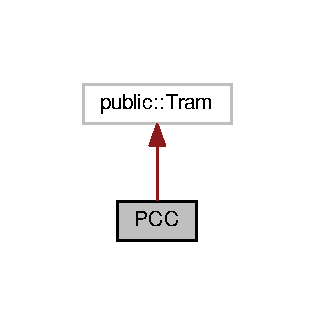
\includegraphics[width=151pt]{classPCC__inherit__graph}
\end{center}
\end{figure}


Collaboration diagram for P\+CC\+:\nopagebreak
\begin{figure}[H]
\begin{center}
\leavevmode
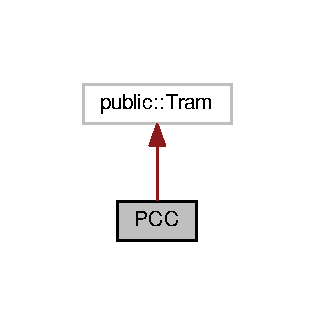
\includegraphics[width=151pt]{classPCC__coll__graph}
\end{center}
\end{figure}
\subsection*{Public Member Functions}
\begin{DoxyCompactItemize}
\item 
string {\bfseries type\+String} ()\hypertarget{classPCC_a6cc8b127dc4790be8e73c974704903eb}{}\label{classPCC_a6cc8b127dc4790be8e73c974704903eb}

\item 
bool {\bfseries is\+Albatros} ()\hypertarget{classPCC_aebc2128b783f1013ec39fa55a2df7276}{}\label{classPCC_aebc2128b783f1013ec39fa55a2df7276}

\end{DoxyCompactItemize}


\subsection{Detailed Description}
This Class contains all the functionalities for the \hyperlink{classPCC}{P\+CC} objects. 

\begin{DoxyAuthor}{Authors}
Loreas Clonen \& Luuk van Sloun 
\end{DoxyAuthor}


The documentation for this class was generated from the following files\+:\begin{DoxyCompactItemize}
\item 
src/\+Tram/P\+C\+C.\+h\item 
src/\+Tram/P\+C\+C.\+cpp\end{DoxyCompactItemize}

\hypertarget{classSpoor}{}\section{Spoor Class Reference}
\label{classSpoor}\index{Spoor@{Spoor}}


This Class contains all the functionalities for the \hyperlink{classSpoor}{Spoor} objects.  




{\ttfamily \#include $<$Spoor.\+h$>$}

\subsection*{Public Member Functions}
\begin{DoxyCompactItemize}
\item 
\hyperlink{classSpoor_a64778a4094d2d9cd3a08cbbef5a11787}{Spoor} ()
\begin{DoxyCompactList}\small\item\em \hyperlink{classSpoor}{Spoor} Default Constructor. \end{DoxyCompactList}\item 
bool \hyperlink{classSpoor_a31982084b33e5946f1e15844b084f62f}{properly\+Initialized} ()
\begin{DoxyCompactList}\small\item\em Returns true if properly initialized, false if not. \end{DoxyCompactList}\item 
int \hyperlink{classSpoor_a17c71f600581bc91b85c92d6628d14c5}{get\+Spoor\+Nr} ()
\begin{DoxyCompactList}\small\item\em Returns the \hyperlink{classSpoor}{Spoor} object\textquotesingle{}s Track Number. \end{DoxyCompactList}\item 
void \hyperlink{classSpoor_af0c947d95aafed41f4fa3c5ec96d2e3c}{set\+Spoor\+Nr} (int spoor\+Nr)
\begin{DoxyCompactList}\small\item\em Sets a new \hyperlink{classSpoor}{Spoor} object\textquotesingle{}s Track Number. \end{DoxyCompactList}\item 
string \hyperlink{classSpoor_af72fa63d73e10bb5d0bb0e15958260d5}{get\+Volgende} ()
\begin{DoxyCompactList}\small\item\em Returns the \hyperlink{classStation}{Station} object\textquotesingle{}s Next \hyperlink{classStation}{Station}. \end{DoxyCompactList}\item 
void \hyperlink{classSpoor_a3f372480028541bed83821716b90da58}{set\+Volgende} (string volgende)
\begin{DoxyCompactList}\small\item\em Sets a new \hyperlink{classSpoor}{Spoor} object\textquotesingle{}s Next \hyperlink{classStation}{Station}. \end{DoxyCompactList}\item 
string \hyperlink{classSpoor_a4c9a290c147e08e5734c662c73b9793c}{get\+Vorige} ()
\begin{DoxyCompactList}\small\item\em Returns the \hyperlink{classStation}{Station} object\textquotesingle{}s Previous \hyperlink{classStation}{Station}. \end{DoxyCompactList}\item 
void \hyperlink{classSpoor_a7f6d776cfd20986866011f1a42a6c762}{set\+Vorige} (string vorige)
\begin{DoxyCompactList}\small\item\em Sets a new \hyperlink{classSpoor}{Spoor} object\textquotesingle{}s Previous \hyperlink{classStation}{Station}. \end{DoxyCompactList}\end{DoxyCompactItemize}


\subsection{Detailed Description}
This Class contains all the functionalities for the \hyperlink{classSpoor}{Spoor} objects. 

\begin{DoxyAuthor}{Authors}
Loreas Clonen \& Luuk van Sloun 
\end{DoxyAuthor}


\subsection{Constructor \& Destructor Documentation}
\index{Spoor@{Spoor}!Spoor@{Spoor}}
\index{Spoor@{Spoor}!Spoor@{Spoor}}
\subsubsection[{\texorpdfstring{Spoor()}{Spoor()}}]{\setlength{\rightskip}{0pt plus 5cm}Spoor\+::\+Spoor (
\begin{DoxyParamCaption}
{}
\end{DoxyParamCaption}
)}\hypertarget{classSpoor_a64778a4094d2d9cd3a08cbbef5a11787}{}\label{classSpoor_a64778a4094d2d9cd3a08cbbef5a11787}


\hyperlink{classSpoor}{Spoor} Default Constructor. 

\begin{DoxyPostcond}{Postcondition}
A new \hyperlink{classSpoor}{Spoor} Object has been created 
\end{DoxyPostcond}


\subsection{Member Function Documentation}
\index{Spoor@{Spoor}!get\+Spoor\+Nr@{get\+Spoor\+Nr}}
\index{get\+Spoor\+Nr@{get\+Spoor\+Nr}!Spoor@{Spoor}}
\subsubsection[{\texorpdfstring{get\+Spoor\+Nr()}{getSpoorNr()}}]{\setlength{\rightskip}{0pt plus 5cm}int Spoor\+::get\+Spoor\+Nr (
\begin{DoxyParamCaption}
{}
\end{DoxyParamCaption}
)}\hypertarget{classSpoor_a17c71f600581bc91b85c92d6628d14c5}{}\label{classSpoor_a17c71f600581bc91b85c92d6628d14c5}


Returns the \hyperlink{classSpoor}{Spoor} object\textquotesingle{}s Track Number. 

\begin{DoxyPrecond}{Precondition}
The \hyperlink{classSpoor}{Spoor} Object has been properly initialized 

The \hyperlink{classSpoor}{Spoor} Object has a non-\/empty member variable spoor\+Nr 
\end{DoxyPrecond}
\begin{DoxyReturn}{Returns}
integer 
\end{DoxyReturn}
\index{Spoor@{Spoor}!get\+Volgende@{get\+Volgende}}
\index{get\+Volgende@{get\+Volgende}!Spoor@{Spoor}}
\subsubsection[{\texorpdfstring{get\+Volgende()}{getVolgende()}}]{\setlength{\rightskip}{0pt plus 5cm}string Spoor\+::get\+Volgende (
\begin{DoxyParamCaption}
{}
\end{DoxyParamCaption}
)}\hypertarget{classSpoor_af72fa63d73e10bb5d0bb0e15958260d5}{}\label{classSpoor_af72fa63d73e10bb5d0bb0e15958260d5}


Returns the \hyperlink{classStation}{Station} object\textquotesingle{}s Next \hyperlink{classStation}{Station}. 

\begin{DoxyPrecond}{Precondition}
The \hyperlink{classSpoor}{Spoor} Object has been properly initialized 

The \hyperlink{classSpoor}{Spoor} Object has a non-\/empty member variable volgende 
\end{DoxyPrecond}
\begin{DoxyReturn}{Returns}
string 
\end{DoxyReturn}
\index{Spoor@{Spoor}!get\+Vorige@{get\+Vorige}}
\index{get\+Vorige@{get\+Vorige}!Spoor@{Spoor}}
\subsubsection[{\texorpdfstring{get\+Vorige()}{getVorige()}}]{\setlength{\rightskip}{0pt plus 5cm}string Spoor\+::get\+Vorige (
\begin{DoxyParamCaption}
{}
\end{DoxyParamCaption}
)}\hypertarget{classSpoor_a4c9a290c147e08e5734c662c73b9793c}{}\label{classSpoor_a4c9a290c147e08e5734c662c73b9793c}


Returns the \hyperlink{classStation}{Station} object\textquotesingle{}s Previous \hyperlink{classStation}{Station}. 

\begin{DoxyPrecond}{Precondition}
The \hyperlink{classSpoor}{Spoor} Object has been properly initialized 

The \hyperlink{classSpoor}{Spoor} Object has a non-\/empty member variable vorige 
\end{DoxyPrecond}
\begin{DoxyReturn}{Returns}
string 
\end{DoxyReturn}
\index{Spoor@{Spoor}!properly\+Initialized@{properly\+Initialized}}
\index{properly\+Initialized@{properly\+Initialized}!Spoor@{Spoor}}
\subsubsection[{\texorpdfstring{properly\+Initialized()}{properlyInitialized()}}]{\setlength{\rightskip}{0pt plus 5cm}bool Spoor\+::properly\+Initialized (
\begin{DoxyParamCaption}
{}
\end{DoxyParamCaption}
)}\hypertarget{classSpoor_a31982084b33e5946f1e15844b084f62f}{}\label{classSpoor_a31982084b33e5946f1e15844b084f62f}


Returns true if properly initialized, false if not. 

\begin{DoxyReturn}{Returns}
boolean 
\end{DoxyReturn}
\index{Spoor@{Spoor}!set\+Spoor\+Nr@{set\+Spoor\+Nr}}
\index{set\+Spoor\+Nr@{set\+Spoor\+Nr}!Spoor@{Spoor}}
\subsubsection[{\texorpdfstring{set\+Spoor\+Nr(int spoor\+Nr)}{setSpoorNr(int spoorNr)}}]{\setlength{\rightskip}{0pt plus 5cm}int Spoor\+::set\+Spoor\+Nr (
\begin{DoxyParamCaption}
\item[{int}]{spoor\+Nr}
\end{DoxyParamCaption}
)}\hypertarget{classSpoor_af0c947d95aafed41f4fa3c5ec96d2e3c}{}\label{classSpoor_af0c947d95aafed41f4fa3c5ec96d2e3c}


Sets a new \hyperlink{classSpoor}{Spoor} object\textquotesingle{}s Track Number. 


\begin{DoxyParams}{Parameters}
{\em spoor\+Nr} & -\/ integer \\
\hline
\end{DoxyParams}
\begin{DoxyPrecond}{Precondition}
The \hyperlink{classSpoor}{Spoor} Object has been properly initialized 

spoor\+Nr is a positive integer 
\end{DoxyPrecond}
\begin{DoxyPostcond}{Postcondition}
The \hyperlink{classSpoor}{Spoor} Object\textquotesingle{}s Track Number is equal to variable spoor\+Nr 
\end{DoxyPostcond}
\index{Spoor@{Spoor}!set\+Volgende@{set\+Volgende}}
\index{set\+Volgende@{set\+Volgende}!Spoor@{Spoor}}
\subsubsection[{\texorpdfstring{set\+Volgende(string volgende)}{setVolgende(string volgende)}}]{\setlength{\rightskip}{0pt plus 5cm}void Spoor\+::set\+Volgende (
\begin{DoxyParamCaption}
\item[{string}]{volgende}
\end{DoxyParamCaption}
)}\hypertarget{classSpoor_a3f372480028541bed83821716b90da58}{}\label{classSpoor_a3f372480028541bed83821716b90da58}


Sets a new \hyperlink{classSpoor}{Spoor} object\textquotesingle{}s Next \hyperlink{classStation}{Station}. 


\begin{DoxyParams}{Parameters}
{\em volgende} & -\/ string \\
\hline
\end{DoxyParams}
\begin{DoxyPrecond}{Precondition}
The \hyperlink{classSpoor}{Spoor} Object has been properly initialized 

volgende is a non-\/empty string 
\end{DoxyPrecond}
\begin{DoxyPostcond}{Postcondition}
The \hyperlink{classSpoor}{Spoor} Object\textquotesingle{}s Next \hyperlink{classStation}{Station} is equal to variable volgende 
\end{DoxyPostcond}
\index{Spoor@{Spoor}!set\+Vorige@{set\+Vorige}}
\index{set\+Vorige@{set\+Vorige}!Spoor@{Spoor}}
\subsubsection[{\texorpdfstring{set\+Vorige(string vorige)}{setVorige(string vorige)}}]{\setlength{\rightskip}{0pt plus 5cm}void Spoor\+::set\+Vorige (
\begin{DoxyParamCaption}
\item[{string}]{vorige}
\end{DoxyParamCaption}
)}\hypertarget{classSpoor_a7f6d776cfd20986866011f1a42a6c762}{}\label{classSpoor_a7f6d776cfd20986866011f1a42a6c762}


Sets a new \hyperlink{classSpoor}{Spoor} object\textquotesingle{}s Previous \hyperlink{classStation}{Station}. 


\begin{DoxyParams}{Parameters}
{\em vorige} & -\/ string \\
\hline
\end{DoxyParams}
\begin{DoxyPrecond}{Precondition}
The \hyperlink{classSpoor}{Spoor} Object has been properly initialized 

vorige is a non-\/empty string 
\end{DoxyPrecond}
\begin{DoxyPostcond}{Postcondition}
The \hyperlink{classSpoor}{Spoor} Object\textquotesingle{}s Next \hyperlink{classStation}{Station} is equal to variable vorige 
\end{DoxyPostcond}


The documentation for this class was generated from the following files\+:\begin{DoxyCompactItemize}
\item 
src/\+Spoor/\hyperlink{Spoor_8h}{Spoor.\+h}\item 
src/\+Spoor/Spoor.\+cpp\end{DoxyCompactItemize}

\hypertarget{classStation}{}\section{Station Class Reference}
\label{classStation}\index{Station@{Station}}


This Class contains all the functionalities for the \hyperlink{classStation}{Station} objects.  




{\ttfamily \#include $<$Station.\+h$>$}

\subsection*{Public Member Functions}
\begin{DoxyCompactItemize}
\item 
\hyperlink{classStation_a73d335726aad1d844d81cda6d9fd74e6}{Station} ()\hypertarget{classStation_a73d335726aad1d844d81cda6d9fd74e6}{}\label{classStation_a73d335726aad1d844d81cda6d9fd74e6}

\begin{DoxyCompactList}\small\item\em \hyperlink{classStation}{Station} Default Constructor. \end{DoxyCompactList}\item 
string \hyperlink{classStation_a7db91849f0d5bab0a4ac0aa4967721cf}{get\+Naam} ()
\begin{DoxyCompactList}\small\item\em Returns the \hyperlink{classStation}{Station} object\textquotesingle{}s name. \end{DoxyCompactList}\item 
void \hyperlink{classStation_a9838301eaa0d45561877bcebc19a663c}{set\+Naam} (string naam)
\begin{DoxyCompactList}\small\item\em Sets a new \hyperlink{classStation}{Station} object\textquotesingle{}s name. \end{DoxyCompactList}\item 
bool \hyperlink{classStation_aab182a50a2992afe0df4412f7de4b73d}{properly\+Initialized} ()
\begin{DoxyCompactList}\small\item\em Returns true if properly initialized, false if not. \end{DoxyCompactList}\item 
string \hyperlink{classStation_aac519858a1ac53608d24d78e4b9231ab}{get\+Type} ()
\begin{DoxyCompactList}\small\item\em Returns the \hyperlink{classStation}{Station} object\textquotesingle{}s type. \end{DoxyCompactList}\item 
void \hyperlink{classStation_a1a38a1c6db22cfda3c5885281252a3b9}{set\+Type} (string type)
\begin{DoxyCompactList}\small\item\em Sets a new \hyperlink{classStation}{Station} object\textquotesingle{}s type. \end{DoxyCompactList}\item 
void \hyperlink{classStation_a9584a65058bdf75254e3a2d79ddcdba1}{add\+Passagier} (string \hyperlink{classPassagier}{Passagier})
\begin{DoxyCompactList}\small\item\em Adds a Passenger to the \hyperlink{classStation}{Station} object\textquotesingle{}s Passenger set. \end{DoxyCompactList}\item 
void \hyperlink{classStation_aa250b3ba3e62c3d433b4c29f6cca38d4}{remove\+Passagier} (string \hyperlink{classPassagier}{Passagier})
\begin{DoxyCompactList}\small\item\em Removes a Passenger from the \hyperlink{classStation}{Station} object\textquotesingle{}s Passenger set. \end{DoxyCompactList}\item 
set$<$ string $>$ \hyperlink{classStation_a3c25e627a9036778a4d6d08ca1454aa6}{get\+Passagier} ()
\begin{DoxyCompactList}\small\item\em Returns the \hyperlink{classStation}{Station} object\textquotesingle{}s Passenger set. \end{DoxyCompactList}\item 
map$<$ int, \hyperlink{classSpoor}{Spoor} $\ast$ $>$ \hyperlink{classStation_a8ee617b13d4d67d0d3d1384d6d33226f}{get\+Sporen} ()
\begin{DoxyCompactList}\small\item\em Returns the \hyperlink{classStation}{Station} object\textquotesingle{}s Tracks map. \end{DoxyCompactList}\item 
void \hyperlink{classStation_a55911b5e0a355f085afd75391827729f}{add\+Spoor} (\hyperlink{classSpoor}{Spoor} $\ast$spoor, int spoor\+Nr)
\begin{DoxyCompactList}\small\item\em Adds a new \hyperlink{classStation}{Station} Track to the Tracks map. \end{DoxyCompactList}\item 
virtual string {\bfseries type\+String} ()\hypertarget{classStation_ad83c424982c3e8e85d446593cc833141}{}\label{classStation_ad83c424982c3e8e85d446593cc833141}

\item 
void {\bfseries set\+Sporen} (map$<$ int, \hyperlink{classSpoor}{Spoor} $\ast$ $>$ sporen)\hypertarget{classStation_a036804467eb7a7c3bf51a90b4ee57eee}{}\label{classStation_a036804467eb7a7c3bf51a90b4ee57eee}

\item 
virtual bool {\bfseries is\+Metrostation} ()\hypertarget{classStation_a6c9833b35ffe26df4a0b163c9186be07}{}\label{classStation_a6c9833b35ffe26df4a0b163c9186be07}

\end{DoxyCompactItemize}


\subsection{Detailed Description}
This Class contains all the functionalities for the \hyperlink{classStation}{Station} objects. 

\begin{DoxyAuthor}{Authors}
Loreas Clonen \& Luuk van Sloun 
\end{DoxyAuthor}


\subsection{Member Function Documentation}
\index{Station@{Station}!add\+Passagier@{add\+Passagier}}
\index{add\+Passagier@{add\+Passagier}!Station@{Station}}
\subsubsection[{\texorpdfstring{add\+Passagier(string Passagier)}{addPassagier(string Passagier)}}]{\setlength{\rightskip}{0pt plus 5cm}void Station\+::add\+Passagier (
\begin{DoxyParamCaption}
\item[{string}]{Passagier}
\end{DoxyParamCaption}
)}\hypertarget{classStation_a9584a65058bdf75254e3a2d79ddcdba1}{}\label{classStation_a9584a65058bdf75254e3a2d79ddcdba1}


Adds a Passenger to the \hyperlink{classStation}{Station} object\textquotesingle{}s Passenger set. 


\begin{DoxyParams}{Parameters}
{\em \hyperlink{classPassagier}{Passagier}} & -\/ string \\
\hline
\end{DoxyParams}
\index{Station@{Station}!add\+Spoor@{add\+Spoor}}
\index{add\+Spoor@{add\+Spoor}!Station@{Station}}
\subsubsection[{\texorpdfstring{add\+Spoor(\+Spoor $\ast$spoor, int spoor\+Nr)}{addSpoor(Spoor *spoor, int spoorNr)}}]{\setlength{\rightskip}{0pt plus 5cm}void Station\+::add\+Spoor (
\begin{DoxyParamCaption}
\item[{{\bf Spoor} $\ast$}]{spoor, }
\item[{int}]{spoor\+Nr}
\end{DoxyParamCaption}
)}\hypertarget{classStation_a55911b5e0a355f085afd75391827729f}{}\label{classStation_a55911b5e0a355f085afd75391827729f}


Adds a new \hyperlink{classStation}{Station} Track to the Tracks map. 


\begin{DoxyParams}{Parameters}
{\em spoor} & -\/ \hyperlink{classSpoor}{Spoor} Pointer \\
\hline
{\em spoor\+Nr} & -\/ integer \\
\hline
\end{DoxyParams}
\index{Station@{Station}!get\+Naam@{get\+Naam}}
\index{get\+Naam@{get\+Naam}!Station@{Station}}
\subsubsection[{\texorpdfstring{get\+Naam()}{getNaam()}}]{\setlength{\rightskip}{0pt plus 5cm}string Station\+::get\+Naam (
\begin{DoxyParamCaption}
{}
\end{DoxyParamCaption}
)}\hypertarget{classStation_a7db91849f0d5bab0a4ac0aa4967721cf}{}\label{classStation_a7db91849f0d5bab0a4ac0aa4967721cf}


Returns the \hyperlink{classStation}{Station} object\textquotesingle{}s name. 

\begin{DoxyReturn}{Returns}
string 
\end{DoxyReturn}
\index{Station@{Station}!get\+Passagier@{get\+Passagier}}
\index{get\+Passagier@{get\+Passagier}!Station@{Station}}
\subsubsection[{\texorpdfstring{get\+Passagier()}{getPassagier()}}]{\setlength{\rightskip}{0pt plus 5cm}set$<$ string $>$ Station\+::get\+Passagier (
\begin{DoxyParamCaption}
{}
\end{DoxyParamCaption}
)}\hypertarget{classStation_a3c25e627a9036778a4d6d08ca1454aa6}{}\label{classStation_a3c25e627a9036778a4d6d08ca1454aa6}


Returns the \hyperlink{classStation}{Station} object\textquotesingle{}s Passenger set. 

\begin{DoxyReturn}{Returns}
passagier -\/ set 
\end{DoxyReturn}
\index{Station@{Station}!get\+Sporen@{get\+Sporen}}
\index{get\+Sporen@{get\+Sporen}!Station@{Station}}
\subsubsection[{\texorpdfstring{get\+Sporen()}{getSporen()}}]{\setlength{\rightskip}{0pt plus 5cm}map$<$ int, {\bf Spoor} $\ast$ $>$ Station\+::get\+Sporen (
\begin{DoxyParamCaption}
{}
\end{DoxyParamCaption}
)}\hypertarget{classStation_a8ee617b13d4d67d0d3d1384d6d33226f}{}\label{classStation_a8ee617b13d4d67d0d3d1384d6d33226f}


Returns the \hyperlink{classStation}{Station} object\textquotesingle{}s Tracks map. 

\begin{DoxyReturn}{Returns}
sporen -\/ map 
\end{DoxyReturn}
\index{Station@{Station}!get\+Type@{get\+Type}}
\index{get\+Type@{get\+Type}!Station@{Station}}
\subsubsection[{\texorpdfstring{get\+Type()}{getType()}}]{\setlength{\rightskip}{0pt plus 5cm}string Station\+::get\+Type (
\begin{DoxyParamCaption}
{}
\end{DoxyParamCaption}
)}\hypertarget{classStation_aac519858a1ac53608d24d78e4b9231ab}{}\label{classStation_aac519858a1ac53608d24d78e4b9231ab}


Returns the \hyperlink{classStation}{Station} object\textquotesingle{}s type. 

\begin{DoxyReturn}{Returns}
string 
\end{DoxyReturn}
\index{Station@{Station}!properly\+Initialized@{properly\+Initialized}}
\index{properly\+Initialized@{properly\+Initialized}!Station@{Station}}
\subsubsection[{\texorpdfstring{properly\+Initialized()}{properlyInitialized()}}]{\setlength{\rightskip}{0pt plus 5cm}bool Station\+::properly\+Initialized (
\begin{DoxyParamCaption}
{}
\end{DoxyParamCaption}
)}\hypertarget{classStation_aab182a50a2992afe0df4412f7de4b73d}{}\label{classStation_aab182a50a2992afe0df4412f7de4b73d}


Returns true if properly initialized, false if not. 

\begin{DoxyReturn}{Returns}
boolean 
\end{DoxyReturn}
\index{Station@{Station}!remove\+Passagier@{remove\+Passagier}}
\index{remove\+Passagier@{remove\+Passagier}!Station@{Station}}
\subsubsection[{\texorpdfstring{remove\+Passagier(string Passagier)}{removePassagier(string Passagier)}}]{\setlength{\rightskip}{0pt plus 5cm}void Station\+::remove\+Passagier (
\begin{DoxyParamCaption}
\item[{string}]{Passagier}
\end{DoxyParamCaption}
)}\hypertarget{classStation_aa250b3ba3e62c3d433b4c29f6cca38d4}{}\label{classStation_aa250b3ba3e62c3d433b4c29f6cca38d4}


Removes a Passenger from the \hyperlink{classStation}{Station} object\textquotesingle{}s Passenger set. 


\begin{DoxyParams}{Parameters}
{\em \hyperlink{classPassagier}{Passagier}} & -\/ string \\
\hline
\end{DoxyParams}
\index{Station@{Station}!set\+Naam@{set\+Naam}}
\index{set\+Naam@{set\+Naam}!Station@{Station}}
\subsubsection[{\texorpdfstring{set\+Naam(string naam)}{setNaam(string naam)}}]{\setlength{\rightskip}{0pt plus 5cm}void Station\+::set\+Naam (
\begin{DoxyParamCaption}
\item[{string}]{naam}
\end{DoxyParamCaption}
)}\hypertarget{classStation_a9838301eaa0d45561877bcebc19a663c}{}\label{classStation_a9838301eaa0d45561877bcebc19a663c}


Sets a new \hyperlink{classStation}{Station} object\textquotesingle{}s name. 


\begin{DoxyParams}{Parameters}
{\em naam} & -\/ string \\
\hline
\end{DoxyParams}
\index{Station@{Station}!set\+Type@{set\+Type}}
\index{set\+Type@{set\+Type}!Station@{Station}}
\subsubsection[{\texorpdfstring{set\+Type(string type)}{setType(string type)}}]{\setlength{\rightskip}{0pt plus 5cm}void Station\+::set\+Type (
\begin{DoxyParamCaption}
\item[{string}]{type}
\end{DoxyParamCaption}
)}\hypertarget{classStation_a1a38a1c6db22cfda3c5885281252a3b9}{}\label{classStation_a1a38a1c6db22cfda3c5885281252a3b9}


Sets a new \hyperlink{classStation}{Station} object\textquotesingle{}s type. 


\begin{DoxyParams}{Parameters}
{\em type} & -\/ string \\
\hline
\end{DoxyParams}


The documentation for this class was generated from the following files\+:\begin{DoxyCompactItemize}
\item 
src/\+Station/\hyperlink{Station_8h}{Station.\+h}\item 
src/\+Station/Station.\+cpp\end{DoxyCompactItemize}

\hypertarget{classSystem}{}\section{System Class Reference}
\label{classSystem}\index{System@{System}}


This Class contains all the functionalities for the \hyperlink{classSystem}{System} objects.  




{\ttfamily \#include $<$System.\+h$>$}

\subsection*{Public Member Functions}
\begin{DoxyCompactItemize}
\item 
\hyperlink{classSystem_ae317936c9bcf1374d61745572e0f2f8a}{System} ()
\begin{DoxyCompactList}\small\item\em \hyperlink{classSystem}{System} Default Constructor. \end{DoxyCompactList}\item 
bool \hyperlink{classSystem_a8532240d722aafc7084ca6047909c8da}{properly\+Initialized} ()
\begin{DoxyCompactList}\small\item\em Returns the system object\textquotesingle{}s properly\+Initialized member. \end{DoxyCompactList}\item 
map$<$ string, \hyperlink{classStation}{Station} $\ast$ $>$ \hyperlink{classSystem_a30d05f13a13f95f580a0e705142fa3ea}{get\+Stations} ()
\begin{DoxyCompactList}\small\item\em Returns the \hyperlink{classSystem}{System} object\textquotesingle{}s stations member. \end{DoxyCompactList}\item 
map$<$ int, \hyperlink{classTram}{Tram} $\ast$ $>$ \hyperlink{classSystem_a7ef5389572f830ddaa61052ce09f48de}{get\+Trams} ()
\begin{DoxyCompactList}\small\item\em Returns the \hyperlink{classSystem}{System} object\textquotesingle{}s trams member. \end{DoxyCompactList}\item 
string \hyperlink{classSystem_afd117849fbf4d7d8dc0f54988589c249}{Output} ()
\begin{DoxyCompactList}\small\item\em Returns a string containing the current \hyperlink{classSystem}{System} lay-\/out. \end{DoxyCompactList}\item 
void \hyperlink{classSystem_a8d73a59e5ca0c23cc36d3bf4b7ac902d}{add\+Station} (string naam, \hyperlink{classStation}{Station} $\ast$station)
\begin{DoxyCompactList}\small\item\em adds a Station$\ast$ to the stations member \end{DoxyCompactList}\item 
void \hyperlink{classSystem_a9c6d16ae38e21499491a7059d67f9284}{add\+Tram} (int lijn\+Nr, \hyperlink{classTram}{Tram} $\ast$tram)
\begin{DoxyCompactList}\small\item\em adds a Tram$\ast$ to the trams member \end{DoxyCompactList}\item 
void \hyperlink{classSystem_a8060d45e6030ee1ad01a11a990bdd1ad}{properlyparsed} ()\hypertarget{classSystem_a8060d45e6030ee1ad01a11a990bdd1ad}{}\label{classSystem_a8060d45e6030ee1ad01a11a990bdd1ad}

\begin{DoxyCompactList}\small\item\em Checks wether or not the system is properly parsed. \end{DoxyCompactList}\item 
void \hyperlink{classSystem_af140010428a79ddde06f3546e7737d86}{set\+Properly\+Parsed} (bool properly\+Parsed)
\begin{DoxyCompactList}\small\item\em Gives a new value to the member properlyparsed. \end{DoxyCompactList}\item 
map$<$ string, \hyperlink{classPassagier}{Passagier} $\ast$ $>$ \hyperlink{classSystem_a25bf1c319312604ce89890fa827f4552}{get\+Passagiers} ()
\begin{DoxyCompactList}\small\item\em Returns the member passagiers. \end{DoxyCompactList}\item 
void \hyperlink{classSystem_ad2a3016a3d4cf9273cf8156f4fc69dfb}{add\+Passagier} (string naam, \hyperlink{classPassagier}{Passagier} $\ast$passagier)
\begin{DoxyCompactList}\small\item\em adds a Passagier$\ast$ to the passagiers member \end{DoxyCompactList}\item 
void \hyperlink{classSystem_ae392bbed93678914f3b0aff18c4a6d4d}{auto\+Simulation} ()
\begin{DoxyCompactList}\small\item\em Simulates the system running. \end{DoxyCompactList}\end{DoxyCompactItemize}


\subsection{Detailed Description}
This Class contains all the functionalities for the \hyperlink{classSystem}{System} objects. 

\begin{DoxyAuthor}{Authors}
Loreas Clonen \& Luuk van Sloun 
\end{DoxyAuthor}


\subsection{Constructor \& Destructor Documentation}
\index{System@{System}!System@{System}}
\index{System@{System}!System@{System}}
\subsubsection[{\texorpdfstring{System()}{System()}}]{\setlength{\rightskip}{0pt plus 5cm}System\+::\+System (
\begin{DoxyParamCaption}
{}
\end{DoxyParamCaption}
)}\hypertarget{classSystem_ae317936c9bcf1374d61745572e0f2f8a}{}\label{classSystem_ae317936c9bcf1374d61745572e0f2f8a}


\hyperlink{classSystem}{System} Default Constructor. 

\begin{DoxyPostcond}{Postcondition}
A new \hyperlink{classSystem}{System} Object has been created 
\end{DoxyPostcond}


\subsection{Member Function Documentation}
\index{System@{System}!add\+Passagier@{add\+Passagier}}
\index{add\+Passagier@{add\+Passagier}!System@{System}}
\subsubsection[{\texorpdfstring{add\+Passagier(string naam, Passagier $\ast$passagier)}{addPassagier(string naam, Passagier *passagier)}}]{\setlength{\rightskip}{0pt plus 5cm}void System\+::add\+Passagier (
\begin{DoxyParamCaption}
\item[{string}]{naam, }
\item[{{\bf Passagier} $\ast$}]{passagier}
\end{DoxyParamCaption}
)}\hypertarget{classSystem_ad2a3016a3d4cf9273cf8156f4fc69dfb}{}\label{classSystem_ad2a3016a3d4cf9273cf8156f4fc69dfb}


adds a Passagier$\ast$ to the passagiers member 


\begin{DoxyParams}{Parameters}
{\em naam} & -\/ string \\
\hline
{\em passagier} & -\/ Passagier$\ast$ \\
\hline
\end{DoxyParams}
\begin{DoxyPrecond}{Precondition}
The \hyperlink{classSystem}{System} object has been properly initialized 

naam is a non-\/empty string, passagier has been properly initialized 
\end{DoxyPrecond}
\begin{DoxyPostcond}{Postcondition}
A new Passenger Object has been added to the \hyperlink{classSystem}{System} Object\textquotesingle{}s Passenger map 
\end{DoxyPostcond}
\index{System@{System}!add\+Station@{add\+Station}}
\index{add\+Station@{add\+Station}!System@{System}}
\subsubsection[{\texorpdfstring{add\+Station(string naam, Station $\ast$station)}{addStation(string naam, Station *station)}}]{\setlength{\rightskip}{0pt plus 5cm}void System\+::add\+Station (
\begin{DoxyParamCaption}
\item[{string}]{naam, }
\item[{{\bf Station} $\ast$}]{station}
\end{DoxyParamCaption}
)}\hypertarget{classSystem_a8d73a59e5ca0c23cc36d3bf4b7ac902d}{}\label{classSystem_a8d73a59e5ca0c23cc36d3bf4b7ac902d}


adds a Station$\ast$ to the stations member 


\begin{DoxyParams}{Parameters}
{\em naam} & -\/ string \\
\hline
{\em station} & -\/ Station$\ast$ \\
\hline
\end{DoxyParams}
\begin{DoxyPrecond}{Precondition}
The \hyperlink{classSystem}{System} Object has been properly initialized 

naam is a non-\/empty string, station has been properly initialized 
\end{DoxyPrecond}
\begin{DoxyPostcond}{Postcondition}
A new \hyperlink{classStation}{Station} Object has been added to the \hyperlink{classSystem}{System} Object\textquotesingle{}s \hyperlink{classStation}{Station} map 
\end{DoxyPostcond}
\index{System@{System}!add\+Tram@{add\+Tram}}
\index{add\+Tram@{add\+Tram}!System@{System}}
\subsubsection[{\texorpdfstring{add\+Tram(int lijn\+Nr, Tram $\ast$tram)}{addTram(int lijnNr, Tram *tram)}}]{\setlength{\rightskip}{0pt plus 5cm}void System\+::add\+Tram (
\begin{DoxyParamCaption}
\item[{int}]{lijn\+Nr, }
\item[{{\bf Tram} $\ast$}]{tram}
\end{DoxyParamCaption}
)}\hypertarget{classSystem_a9c6d16ae38e21499491a7059d67f9284}{}\label{classSystem_a9c6d16ae38e21499491a7059d67f9284}


adds a Tram$\ast$ to the trams member 


\begin{DoxyParams}{Parameters}
{\em lijn\+Nr} & -\/ int \\
\hline
{\em tram} & -\/ Tram$\ast$ \\
\hline
\end{DoxyParams}
\begin{DoxyPrecond}{Precondition}
The \hyperlink{classSystem}{System} Object has been properly initialized 

lijn\+Nr is a positive integer, tram has been properly initialized 
\end{DoxyPrecond}
\begin{DoxyPostcond}{Postcondition}
A new \hyperlink{classTram}{Tram} Object has been added to the \hyperlink{classSystem}{System} Object\textquotesingle{}s \hyperlink{classTram}{Tram} map 
\end{DoxyPostcond}
\index{System@{System}!auto\+Simulation@{auto\+Simulation}}
\index{auto\+Simulation@{auto\+Simulation}!System@{System}}
\subsubsection[{\texorpdfstring{auto\+Simulation()}{autoSimulation()}}]{\setlength{\rightskip}{0pt plus 5cm}void System\+::auto\+Simulation (
\begin{DoxyParamCaption}
{}
\end{DoxyParamCaption}
)}\hypertarget{classSystem_ae392bbed93678914f3b0aff18c4a6d4d}{}\label{classSystem_ae392bbed93678914f3b0aff18c4a6d4d}


Simulates the system running. 

\begin{DoxyPrecond}{Precondition}
The \hyperlink{classSystem}{System} Object has been properly initialized 
\end{DoxyPrecond}
\index{System@{System}!get\+Passagiers@{get\+Passagiers}}
\index{get\+Passagiers@{get\+Passagiers}!System@{System}}
\subsubsection[{\texorpdfstring{get\+Passagiers()}{getPassagiers()}}]{\setlength{\rightskip}{0pt plus 5cm}map$<$ string, {\bf Passagier} $\ast$ $>$ System\+::get\+Passagiers (
\begin{DoxyParamCaption}
{}
\end{DoxyParamCaption}
)}\hypertarget{classSystem_a25bf1c319312604ce89890fa827f4552}{}\label{classSystem_a25bf1c319312604ce89890fa827f4552}


Returns the member passagiers. 

\begin{DoxyPrecond}{Precondition}
The \hyperlink{classSystem}{System} Object has been properly initialized 

The \hyperlink{classSystem}{System} Object has a non-\/empty member variable passagiers 
\end{DoxyPrecond}
\begin{DoxyReturn}{Returns}
map$<$string, Passagier$\ast$$>$ 
\end{DoxyReturn}
\index{System@{System}!get\+Stations@{get\+Stations}}
\index{get\+Stations@{get\+Stations}!System@{System}}
\subsubsection[{\texorpdfstring{get\+Stations()}{getStations()}}]{\setlength{\rightskip}{0pt plus 5cm}map$<$ string, {\bf Station} $\ast$ $>$ System\+::get\+Stations (
\begin{DoxyParamCaption}
{}
\end{DoxyParamCaption}
)}\hypertarget{classSystem_a30d05f13a13f95f580a0e705142fa3ea}{}\label{classSystem_a30d05f13a13f95f580a0e705142fa3ea}


Returns the \hyperlink{classSystem}{System} object\textquotesingle{}s stations member. 

\begin{DoxyPrecond}{Precondition}
The \hyperlink{classSystem}{System} Object has been properly initialized 

The \hyperlink{classSystem}{System} Object has a non-\/empty member variable stations 
\end{DoxyPrecond}
\begin{DoxyReturn}{Returns}
map$<$string, Tram$\ast$$>$ 
\end{DoxyReturn}
\index{System@{System}!get\+Trams@{get\+Trams}}
\index{get\+Trams@{get\+Trams}!System@{System}}
\subsubsection[{\texorpdfstring{get\+Trams()}{getTrams()}}]{\setlength{\rightskip}{0pt plus 5cm}map$<$ string, {\bf Tram} $\ast$ $>$ System\+::get\+Trams (
\begin{DoxyParamCaption}
{}
\end{DoxyParamCaption}
)}\hypertarget{classSystem_a7ef5389572f830ddaa61052ce09f48de}{}\label{classSystem_a7ef5389572f830ddaa61052ce09f48de}


Returns the \hyperlink{classSystem}{System} object\textquotesingle{}s trams member. 

\begin{DoxyPrecond}{Precondition}
The \hyperlink{classSystem}{System} Object has been properly initialized 

The \hyperlink{classSystem}{System} Object has a non-\/empty member variable trams 
\end{DoxyPrecond}
\begin{DoxyReturn}{Returns}
map$<$string, Tram$\ast$$>$ 
\end{DoxyReturn}
\index{System@{System}!Output@{Output}}
\index{Output@{Output}!System@{System}}
\subsubsection[{\texorpdfstring{Output()}{Output()}}]{\setlength{\rightskip}{0pt plus 5cm}string System\+::\+Output (
\begin{DoxyParamCaption}
{}
\end{DoxyParamCaption}
)}\hypertarget{classSystem_afd117849fbf4d7d8dc0f54988589c249}{}\label{classSystem_afd117849fbf4d7d8dc0f54988589c249}


Returns a string containing the current \hyperlink{classSystem}{System} lay-\/out. 

\begin{DoxyPrecond}{Precondition}
The \hyperlink{classSystem}{System} Object has been properly initialized 
\end{DoxyPrecond}
\begin{DoxyReturn}{Returns}
string 
\end{DoxyReturn}
\index{System@{System}!properly\+Initialized@{properly\+Initialized}}
\index{properly\+Initialized@{properly\+Initialized}!System@{System}}
\subsubsection[{\texorpdfstring{properly\+Initialized()}{properlyInitialized()}}]{\setlength{\rightskip}{0pt plus 5cm}bool System\+::properly\+Initialized (
\begin{DoxyParamCaption}
{}
\end{DoxyParamCaption}
)}\hypertarget{classSystem_a8532240d722aafc7084ca6047909c8da}{}\label{classSystem_a8532240d722aafc7084ca6047909c8da}


Returns the system object\textquotesingle{}s properly\+Initialized member. 

\begin{DoxyReturn}{Returns}
bool 
\end{DoxyReturn}
\index{System@{System}!set\+Properly\+Parsed@{set\+Properly\+Parsed}}
\index{set\+Properly\+Parsed@{set\+Properly\+Parsed}!System@{System}}
\subsubsection[{\texorpdfstring{set\+Properly\+Parsed(bool properly\+Parsed)}{setProperlyParsed(bool properlyParsed)}}]{\setlength{\rightskip}{0pt plus 5cm}void System\+::set\+Properly\+Parsed (
\begin{DoxyParamCaption}
\item[{bool}]{properlyparsed}
\end{DoxyParamCaption}
)}\hypertarget{classSystem_af140010428a79ddde06f3546e7737d86}{}\label{classSystem_af140010428a79ddde06f3546e7737d86}


Gives a new value to the member properlyparsed. 

\begin{DoxyPostcond}{Postcondition}
The \hyperlink{classSystem}{System} Object\textquotesingle{}s member variable properly\+Parsed is equal to variable properly\+Parsed 
\end{DoxyPostcond}


The documentation for this class was generated from the following files\+:\begin{DoxyCompactItemize}
\item 
src/\+System/\hyperlink{System_8h}{System.\+h}\item 
src/\+System/System.\+cpp\end{DoxyCompactItemize}

\hypertarget{classTiXmlAttribute}{}\section{Ti\+Xml\+Attribute Class Reference}
\label{classTiXmlAttribute}\index{Ti\+Xml\+Attribute@{Ti\+Xml\+Attribute}}


{\ttfamily \#include $<$tinyxml.\+h$>$}



Inheritance diagram for Ti\+Xml\+Attribute\+:\nopagebreak
\begin{figure}[H]
\begin{center}
\leavevmode
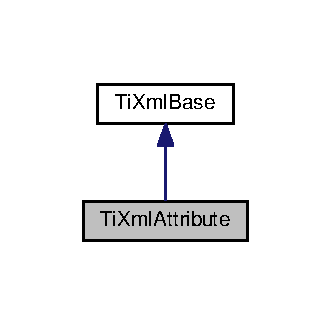
\includegraphics[width=159pt]{classTiXmlAttribute__inherit__graph}
\end{center}
\end{figure}


Collaboration diagram for Ti\+Xml\+Attribute\+:\nopagebreak
\begin{figure}[H]
\begin{center}
\leavevmode
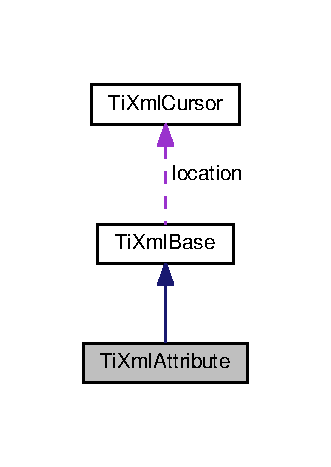
\includegraphics[width=159pt]{classTiXmlAttribute__coll__graph}
\end{center}
\end{figure}
\subsection*{Public Member Functions}
\begin{DoxyCompactItemize}
\item 
\hyperlink{classTiXmlAttribute_a9cfa3c8179873fd485d83003b114f8e1}{Ti\+Xml\+Attribute} ()\hypertarget{classTiXmlAttribute_a9cfa3c8179873fd485d83003b114f8e1}{}\label{classTiXmlAttribute_a9cfa3c8179873fd485d83003b114f8e1}

\begin{DoxyCompactList}\small\item\em Construct an empty attribute. \end{DoxyCompactList}\item 
\hyperlink{classTiXmlAttribute_a759d0b76fb8fcf765ecab243bc14f05e}{Ti\+Xml\+Attribute} (const char $\ast$\+\_\+name, const char $\ast$\+\_\+value)\hypertarget{classTiXmlAttribute_a759d0b76fb8fcf765ecab243bc14f05e}{}\label{classTiXmlAttribute_a759d0b76fb8fcf765ecab243bc14f05e}

\begin{DoxyCompactList}\small\item\em Construct an attribute with a name and value. \end{DoxyCompactList}\item 
const char $\ast$ \hyperlink{classTiXmlAttribute_a298a57287d305904ba6bd96ae6f78d3d}{Name} () const \hypertarget{classTiXmlAttribute_a298a57287d305904ba6bd96ae6f78d3d}{}\label{classTiXmlAttribute_a298a57287d305904ba6bd96ae6f78d3d}

\begin{DoxyCompactList}\small\item\em Return the name of this attribute. \end{DoxyCompactList}\item 
const char $\ast$ \hyperlink{classTiXmlAttribute_a0f874490eac8ca00ee0070765d0e97e3}{Value} () const \hypertarget{classTiXmlAttribute_a0f874490eac8ca00ee0070765d0e97e3}{}\label{classTiXmlAttribute_a0f874490eac8ca00ee0070765d0e97e3}

\begin{DoxyCompactList}\small\item\em Return the value of this attribute. \end{DoxyCompactList}\item 
int \hyperlink{classTiXmlAttribute_aa1a20ad59dc7e89a0ab265396360d50f}{Int\+Value} () const \hypertarget{classTiXmlAttribute_aa1a20ad59dc7e89a0ab265396360d50f}{}\label{classTiXmlAttribute_aa1a20ad59dc7e89a0ab265396360d50f}

\begin{DoxyCompactList}\small\item\em Return the value of this attribute, converted to an integer. \end{DoxyCompactList}\item 
double \hyperlink{classTiXmlAttribute_a2880ddef53fc7522c99535273954d230}{Double\+Value} () const \hypertarget{classTiXmlAttribute_a2880ddef53fc7522c99535273954d230}{}\label{classTiXmlAttribute_a2880ddef53fc7522c99535273954d230}

\begin{DoxyCompactList}\small\item\em Return the value of this attribute, converted to a double. \end{DoxyCompactList}\item 
const T\+I\+X\+M\+L\+\_\+\+S\+T\+R\+I\+NG \& {\bfseries Name\+T\+Str} () const \hypertarget{classTiXmlAttribute_a64cee17bceb8232eb0736d26dd082d79}{}\label{classTiXmlAttribute_a64cee17bceb8232eb0736d26dd082d79}

\item 
int \hyperlink{classTiXmlAttribute_ad6c93088ee21af41a107931223339344}{Query\+Int\+Value} (int $\ast$\+\_\+value) const 
\item 
int \hyperlink{classTiXmlAttribute_ac87b2a8489906a5d7aa2875f20be3513}{Query\+Double\+Value} (double $\ast$\+\_\+value) const \hypertarget{classTiXmlAttribute_ac87b2a8489906a5d7aa2875f20be3513}{}\label{classTiXmlAttribute_ac87b2a8489906a5d7aa2875f20be3513}

\begin{DoxyCompactList}\small\item\em Query\+Double\+Value examines the value string. See \hyperlink{classTiXmlAttribute_ad6c93088ee21af41a107931223339344}{Query\+Int\+Value()}. \end{DoxyCompactList}\item 
void \hyperlink{classTiXmlAttribute_ab7fa3d21ff8d7c5764cf9af15b667a99}{Set\+Name} (const char $\ast$\+\_\+name)\hypertarget{classTiXmlAttribute_ab7fa3d21ff8d7c5764cf9af15b667a99}{}\label{classTiXmlAttribute_ab7fa3d21ff8d7c5764cf9af15b667a99}

\begin{DoxyCompactList}\small\item\em Set the name of this attribute. \end{DoxyCompactList}\item 
void \hyperlink{classTiXmlAttribute_a2dae44178f668b3cb48101be4f2236a0}{Set\+Value} (const char $\ast$\+\_\+value)\hypertarget{classTiXmlAttribute_a2dae44178f668b3cb48101be4f2236a0}{}\label{classTiXmlAttribute_a2dae44178f668b3cb48101be4f2236a0}

\begin{DoxyCompactList}\small\item\em Set the value. \end{DoxyCompactList}\item 
void \hyperlink{classTiXmlAttribute_a7e065df640116a62ea4f4b7da5449cc8}{Set\+Int\+Value} (int \+\_\+value)\hypertarget{classTiXmlAttribute_a7e065df640116a62ea4f4b7da5449cc8}{}\label{classTiXmlAttribute_a7e065df640116a62ea4f4b7da5449cc8}

\begin{DoxyCompactList}\small\item\em Set the value from an integer. \end{DoxyCompactList}\item 
void \hyperlink{classTiXmlAttribute_a0316da31373496c4368ad549bf711394}{Set\+Double\+Value} (double \+\_\+value)\hypertarget{classTiXmlAttribute_a0316da31373496c4368ad549bf711394}{}\label{classTiXmlAttribute_a0316da31373496c4368ad549bf711394}

\begin{DoxyCompactList}\small\item\em Set the value from a double. \end{DoxyCompactList}\item 
const \hyperlink{classTiXmlAttribute}{Ti\+Xml\+Attribute} $\ast$ \hyperlink{classTiXmlAttribute_a776478980776a024f7c2846eec640f65}{Next} () const \hypertarget{classTiXmlAttribute_a776478980776a024f7c2846eec640f65}{}\label{classTiXmlAttribute_a776478980776a024f7c2846eec640f65}

\begin{DoxyCompactList}\small\item\em Get the next sibling attribute in the D\+OM. Returns null at end. \end{DoxyCompactList}\item 
\hyperlink{classTiXmlAttribute}{Ti\+Xml\+Attribute} $\ast$ {\bfseries Next} ()\hypertarget{classTiXmlAttribute_a138320aa7793b148ba7e5bd0a0ea4db6}{}\label{classTiXmlAttribute_a138320aa7793b148ba7e5bd0a0ea4db6}

\item 
const \hyperlink{classTiXmlAttribute}{Ti\+Xml\+Attribute} $\ast$ \hyperlink{classTiXmlAttribute_a54a5f8730c7b02b9a41b74e12e27fe86}{Previous} () const \hypertarget{classTiXmlAttribute_a54a5f8730c7b02b9a41b74e12e27fe86}{}\label{classTiXmlAttribute_a54a5f8730c7b02b9a41b74e12e27fe86}

\begin{DoxyCompactList}\small\item\em Get the previous sibling attribute in the D\+OM. Returns null at beginning. \end{DoxyCompactList}\item 
\hyperlink{classTiXmlAttribute}{Ti\+Xml\+Attribute} $\ast$ {\bfseries Previous} ()\hypertarget{classTiXmlAttribute_ae4dabc932cba945ed1e92fec5f121193}{}\label{classTiXmlAttribute_ae4dabc932cba945ed1e92fec5f121193}

\item 
bool {\bfseries operator==} (const \hyperlink{classTiXmlAttribute}{Ti\+Xml\+Attribute} \&rhs) const \hypertarget{classTiXmlAttribute_ae48c2a65b520d453914ce4e845d607cf}{}\label{classTiXmlAttribute_ae48c2a65b520d453914ce4e845d607cf}

\item 
bool {\bfseries operator$<$} (const \hyperlink{classTiXmlAttribute}{Ti\+Xml\+Attribute} \&rhs) const \hypertarget{classTiXmlAttribute_adb8b6f2cad5948e73e383182e7ce10de}{}\label{classTiXmlAttribute_adb8b6f2cad5948e73e383182e7ce10de}

\item 
bool {\bfseries operator$>$} (const \hyperlink{classTiXmlAttribute}{Ti\+Xml\+Attribute} \&rhs) const \hypertarget{classTiXmlAttribute_a867562769ef9778c1690cd373246b05b}{}\label{classTiXmlAttribute_a867562769ef9778c1690cd373246b05b}

\item 
virtual const char $\ast$ {\bfseries Parse} (const char $\ast$p, \hyperlink{classTiXmlParsingData}{Ti\+Xml\+Parsing\+Data} $\ast$data, Ti\+Xml\+Encoding encoding)\hypertarget{classTiXmlAttribute_ad62774421b814894b995af3b5d231dda}{}\label{classTiXmlAttribute_ad62774421b814894b995af3b5d231dda}

\item 
virtual void \hyperlink{classTiXmlAttribute_acc04956c1d5c4c31fe74f7a7528d109a}{Print} (F\+I\+LE $\ast$cfile, int depth) const 
\item 
void {\bfseries Print} (F\+I\+LE $\ast$cfile, int depth, T\+I\+X\+M\+L\+\_\+\+S\+T\+R\+I\+NG $\ast$str) const \hypertarget{classTiXmlAttribute_a19e6b6862a80b188571c47947e88d030}{}\label{classTiXmlAttribute_a19e6b6862a80b188571c47947e88d030}

\item 
void {\bfseries Set\+Document} (\hyperlink{classTiXmlDocument}{Ti\+Xml\+Document} $\ast$doc)\hypertarget{classTiXmlAttribute_ac12a94d4548302afb12f488ba101f7d1}{}\label{classTiXmlAttribute_ac12a94d4548302afb12f488ba101f7d1}

\end{DoxyCompactItemize}
\subsection*{Friends}
\begin{DoxyCompactItemize}
\item 
class {\bfseries Ti\+Xml\+Attribute\+Set}\hypertarget{classTiXmlAttribute_a35a7b7f89f708527677d5078d41ce0bf}{}\label{classTiXmlAttribute_a35a7b7f89f708527677d5078d41ce0bf}

\end{DoxyCompactItemize}
\subsection*{Additional Inherited Members}


\subsection{Detailed Description}
An attribute is a name-\/value pair. Elements have an arbitrary number of attributes, each with a unique name.

\begin{DoxyNote}{Note}
The attributes are not Ti\+Xml\+Nodes, since they are not part of the tiny\+X\+ML document object model. There are other suggested ways to look at this problem. 
\end{DoxyNote}


\subsection{Member Function Documentation}
\index{Ti\+Xml\+Attribute@{Ti\+Xml\+Attribute}!Print@{Print}}
\index{Print@{Print}!Ti\+Xml\+Attribute@{Ti\+Xml\+Attribute}}
\subsubsection[{\texorpdfstring{Print(\+F\+I\+L\+E $\ast$cfile, int depth) const }{Print(FILE *cfile, int depth) const }}]{\setlength{\rightskip}{0pt plus 5cm}virtual void Ti\+Xml\+Attribute\+::\+Print (
\begin{DoxyParamCaption}
\item[{F\+I\+LE $\ast$}]{cfile, }
\item[{int}]{depth}
\end{DoxyParamCaption}
) const\hspace{0.3cm}{\ttfamily [inline]}, {\ttfamily [virtual]}}\hypertarget{classTiXmlAttribute_acc04956c1d5c4c31fe74f7a7528d109a}{}\label{classTiXmlAttribute_acc04956c1d5c4c31fe74f7a7528d109a}
All Tiny\+Xml classes can print themselves to a filestream or the string class (\hyperlink{classTiXmlString}{Ti\+Xml\+String} in non-\/\+S\+TL mode, std\+::string in S\+TL mode.) Either or both cfile and str can be null.

This is a formatted print, and will insert tabs and newlines.

(For an unformatted stream, use the $<$$<$ operator.) 

Implements \hyperlink{classTiXmlBase_a0de56b3f2ef14c65091a3b916437b512}{Ti\+Xml\+Base}.

\index{Ti\+Xml\+Attribute@{Ti\+Xml\+Attribute}!Query\+Int\+Value@{Query\+Int\+Value}}
\index{Query\+Int\+Value@{Query\+Int\+Value}!Ti\+Xml\+Attribute@{Ti\+Xml\+Attribute}}
\subsubsection[{\texorpdfstring{Query\+Int\+Value(int $\ast$\+\_\+value) const }{QueryIntValue(int *_value) const }}]{\setlength{\rightskip}{0pt plus 5cm}int Ti\+Xml\+Attribute\+::\+Query\+Int\+Value (
\begin{DoxyParamCaption}
\item[{int $\ast$}]{\+\_\+value}
\end{DoxyParamCaption}
) const}\hypertarget{classTiXmlAttribute_ad6c93088ee21af41a107931223339344}{}\label{classTiXmlAttribute_ad6c93088ee21af41a107931223339344}
Query\+Int\+Value examines the value string. It is an alternative to the \hyperlink{classTiXmlAttribute_aa1a20ad59dc7e89a0ab265396360d50f}{Int\+Value()} method with richer error checking. If the value is an integer, it is stored in \textquotesingle{}value\textquotesingle{} and the call returns T\+I\+X\+M\+L\+\_\+\+S\+U\+C\+C\+E\+SS. If it is not an integer, it returns T\+I\+X\+M\+L\+\_\+\+W\+R\+O\+N\+G\+\_\+\+T\+Y\+PE.

A specialized but useful call. Note that for success it returns 0, which is the opposite of almost all other Tiny\+Xml calls. 

The documentation for this class was generated from the following files\+:\begin{DoxyCompactItemize}
\item 
src/tinyxml.\+h\item 
src/tinyxml.\+cpp\item 
src/tinyxmlparser.\+cpp\end{DoxyCompactItemize}

\hypertarget{classTiXmlAttributeSet}{}\section{Ti\+Xml\+Attribute\+Set Class Reference}
\label{classTiXmlAttributeSet}\index{Ti\+Xml\+Attribute\+Set@{Ti\+Xml\+Attribute\+Set}}
\subsection*{Public Member Functions}
\begin{DoxyCompactItemize}
\item 
void {\bfseries Add} (\hyperlink{classTiXmlAttribute}{Ti\+Xml\+Attribute} $\ast$attribute)\hypertarget{classTiXmlAttributeSet_a745e50ddaae3bee93e4589321e0b9c1a}{}\label{classTiXmlAttributeSet_a745e50ddaae3bee93e4589321e0b9c1a}

\item 
void {\bfseries Remove} (\hyperlink{classTiXmlAttribute}{Ti\+Xml\+Attribute} $\ast$attribute)\hypertarget{classTiXmlAttributeSet_a924a73d071f2573f9060f0be57879c57}{}\label{classTiXmlAttributeSet_a924a73d071f2573f9060f0be57879c57}

\item 
const \hyperlink{classTiXmlAttribute}{Ti\+Xml\+Attribute} $\ast$ {\bfseries First} () const \hypertarget{classTiXmlAttributeSet_ae0636e88cedd4b09d61c451860f68598}{}\label{classTiXmlAttributeSet_ae0636e88cedd4b09d61c451860f68598}

\item 
\hyperlink{classTiXmlAttribute}{Ti\+Xml\+Attribute} $\ast$ {\bfseries First} ()\hypertarget{classTiXmlAttributeSet_a99703bb08ca2aece2d7ef835de339ba0}{}\label{classTiXmlAttributeSet_a99703bb08ca2aece2d7ef835de339ba0}

\item 
const \hyperlink{classTiXmlAttribute}{Ti\+Xml\+Attribute} $\ast$ {\bfseries Last} () const \hypertarget{classTiXmlAttributeSet_a7b3f3ccf39a97bc25539d3fcc540296a}{}\label{classTiXmlAttributeSet_a7b3f3ccf39a97bc25539d3fcc540296a}

\item 
\hyperlink{classTiXmlAttribute}{Ti\+Xml\+Attribute} $\ast$ {\bfseries Last} ()\hypertarget{classTiXmlAttributeSet_ab4c4edfb2d74f6ea31aae096743bd6e0}{}\label{classTiXmlAttributeSet_ab4c4edfb2d74f6ea31aae096743bd6e0}

\item 
\hyperlink{classTiXmlAttribute}{Ti\+Xml\+Attribute} $\ast$ {\bfseries Find} (const char $\ast$\+\_\+name) const \hypertarget{classTiXmlAttributeSet_af3675cc2bfd0aea153cda1cfcdd1f77e}{}\label{classTiXmlAttributeSet_af3675cc2bfd0aea153cda1cfcdd1f77e}

\item 
\hyperlink{classTiXmlAttribute}{Ti\+Xml\+Attribute} $\ast$ {\bfseries Find\+Or\+Create} (const char $\ast$\+\_\+name)\hypertarget{classTiXmlAttributeSet_a5e28f5d32f048fba85d04dc317495bdc}{}\label{classTiXmlAttributeSet_a5e28f5d32f048fba85d04dc317495bdc}

\end{DoxyCompactItemize}


The documentation for this class was generated from the following files\+:\begin{DoxyCompactItemize}
\item 
src/tinyxml/tinyxml.\+h\item 
src/tinyxml/tinyxml.\+cpp\end{DoxyCompactItemize}

\hypertarget{classTiXmlBase}{}\section{Ti\+Xml\+Base Class Reference}
\label{classTiXmlBase}\index{Ti\+Xml\+Base@{Ti\+Xml\+Base}}


{\ttfamily \#include $<$tinyxml.\+h$>$}



Inheritance diagram for Ti\+Xml\+Base\+:\nopagebreak
\begin{figure}[H]
\begin{center}
\leavevmode
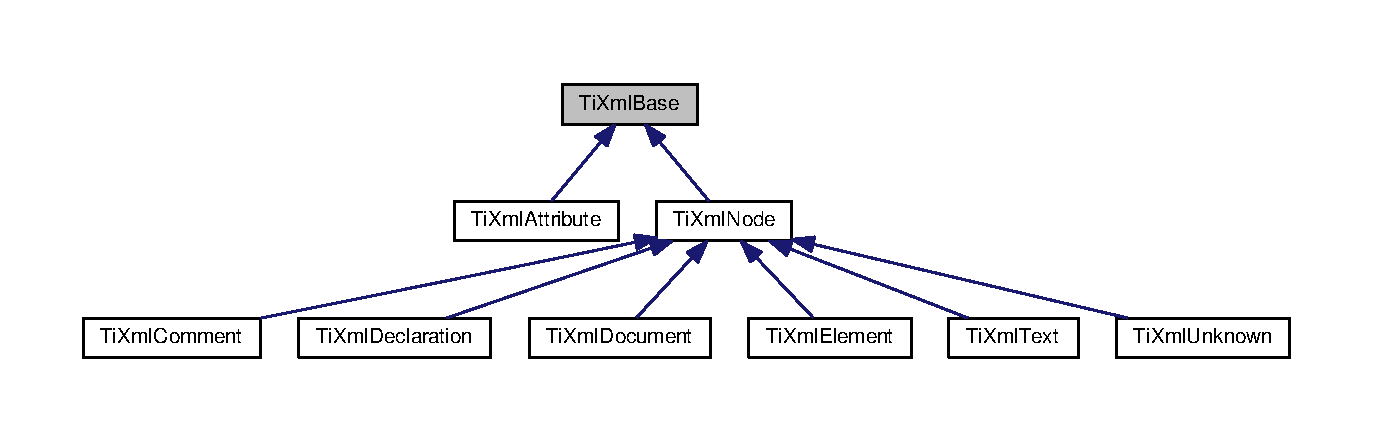
\includegraphics[width=350pt]{classTiXmlBase__inherit__graph}
\end{center}
\end{figure}


Collaboration diagram for Ti\+Xml\+Base\+:\nopagebreak
\begin{figure}[H]
\begin{center}
\leavevmode
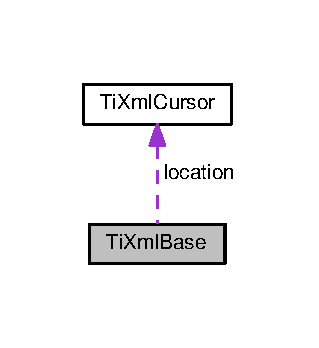
\includegraphics[width=153pt]{classTiXmlBase__coll__graph}
\end{center}
\end{figure}
\subsection*{Public Types}
\begin{DoxyCompactItemize}
\item 
enum \{ \\*
{\bfseries T\+I\+X\+M\+L\+\_\+\+N\+O\+\_\+\+E\+R\+R\+OR} = 0, 
{\bfseries T\+I\+X\+M\+L\+\_\+\+E\+R\+R\+OR}, 
{\bfseries T\+I\+X\+M\+L\+\_\+\+E\+R\+R\+O\+R\+\_\+\+O\+P\+E\+N\+I\+N\+G\+\_\+\+F\+I\+LE}, 
{\bfseries T\+I\+X\+M\+L\+\_\+\+E\+R\+R\+O\+R\+\_\+\+P\+A\+R\+S\+I\+N\+G\+\_\+\+E\+L\+E\+M\+E\+NT}, 
\\*
{\bfseries T\+I\+X\+M\+L\+\_\+\+E\+R\+R\+O\+R\+\_\+\+F\+A\+I\+L\+E\+D\+\_\+\+T\+O\+\_\+\+R\+E\+A\+D\+\_\+\+E\+L\+E\+M\+E\+N\+T\+\_\+\+N\+A\+ME}, 
{\bfseries T\+I\+X\+M\+L\+\_\+\+E\+R\+R\+O\+R\+\_\+\+R\+E\+A\+D\+I\+N\+G\+\_\+\+E\+L\+E\+M\+E\+N\+T\+\_\+\+V\+A\+L\+UE}, 
{\bfseries T\+I\+X\+M\+L\+\_\+\+E\+R\+R\+O\+R\+\_\+\+R\+E\+A\+D\+I\+N\+G\+\_\+\+A\+T\+T\+R\+I\+B\+U\+T\+ES}, 
{\bfseries T\+I\+X\+M\+L\+\_\+\+E\+R\+R\+O\+R\+\_\+\+P\+A\+R\+S\+I\+N\+G\+\_\+\+E\+M\+P\+TY}, 
\\*
{\bfseries T\+I\+X\+M\+L\+\_\+\+E\+R\+R\+O\+R\+\_\+\+R\+E\+A\+D\+I\+N\+G\+\_\+\+E\+N\+D\+\_\+\+T\+AG}, 
{\bfseries T\+I\+X\+M\+L\+\_\+\+E\+R\+R\+O\+R\+\_\+\+P\+A\+R\+S\+I\+N\+G\+\_\+\+U\+N\+K\+N\+O\+WN}, 
{\bfseries T\+I\+X\+M\+L\+\_\+\+E\+R\+R\+O\+R\+\_\+\+P\+A\+R\+S\+I\+N\+G\+\_\+\+C\+O\+M\+M\+E\+NT}, 
{\bfseries T\+I\+X\+M\+L\+\_\+\+E\+R\+R\+O\+R\+\_\+\+P\+A\+R\+S\+I\+N\+G\+\_\+\+D\+E\+C\+L\+A\+R\+A\+T\+I\+ON}, 
\\*
{\bfseries T\+I\+X\+M\+L\+\_\+\+E\+R\+R\+O\+R\+\_\+\+D\+O\+C\+U\+M\+E\+N\+T\+\_\+\+E\+M\+P\+TY}, 
{\bfseries T\+I\+X\+M\+L\+\_\+\+E\+R\+R\+O\+R\+\_\+\+E\+M\+B\+E\+D\+D\+E\+D\+\_\+\+N\+U\+LL}, 
{\bfseries T\+I\+X\+M\+L\+\_\+\+E\+R\+R\+O\+R\+\_\+\+P\+A\+R\+S\+I\+N\+G\+\_\+\+C\+D\+A\+TA}, 
{\bfseries T\+I\+X\+M\+L\+\_\+\+E\+R\+R\+O\+R\+\_\+\+D\+O\+C\+U\+M\+E\+N\+T\+\_\+\+T\+O\+P\+\_\+\+O\+N\+LY}, 
\\*
{\bfseries T\+I\+X\+M\+L\+\_\+\+E\+R\+R\+O\+R\+\_\+\+S\+T\+R\+I\+N\+G\+\_\+\+C\+O\+U\+NT}
 \}\hypertarget{classTiXmlBase_a9a7e9344415956ab96e8c75f6a0bbd48}{}\label{classTiXmlBase_a9a7e9344415956ab96e8c75f6a0bbd48}

\end{DoxyCompactItemize}
\subsection*{Public Member Functions}
\begin{DoxyCompactItemize}
\item 
virtual void \hyperlink{classTiXmlBase_a0de56b3f2ef14c65091a3b916437b512}{Print} (F\+I\+LE $\ast$cfile, int depth) const =0
\item 
int \hyperlink{classTiXmlBase_a024bceb070188df92c2a8d8852dd0853}{Row} () const 
\item 
int \hyperlink{classTiXmlBase_ab54bfb9b70fe6dd276e7b279cab7f003}{Column} () const \hypertarget{classTiXmlBase_ab54bfb9b70fe6dd276e7b279cab7f003}{}\label{classTiXmlBase_ab54bfb9b70fe6dd276e7b279cab7f003}

\begin{DoxyCompactList}\small\item\em See \hyperlink{classTiXmlBase_a024bceb070188df92c2a8d8852dd0853}{Row()} \end{DoxyCompactList}\item 
void \hyperlink{classTiXmlBase_ac6b3e0f790930d4970ec30764e937b5d}{Set\+User\+Data} (void $\ast$user)\hypertarget{classTiXmlBase_ac6b3e0f790930d4970ec30764e937b5d}{}\label{classTiXmlBase_ac6b3e0f790930d4970ec30764e937b5d}

\begin{DoxyCompactList}\small\item\em Set a pointer to arbitrary user data. \end{DoxyCompactList}\item 
void $\ast$ \hyperlink{classTiXmlBase_a6559a530ca6763fc301a14d77ed28c17}{Get\+User\+Data} ()\hypertarget{classTiXmlBase_a6559a530ca6763fc301a14d77ed28c17}{}\label{classTiXmlBase_a6559a530ca6763fc301a14d77ed28c17}

\begin{DoxyCompactList}\small\item\em Get a pointer to arbitrary user data. \end{DoxyCompactList}\item 
const void $\ast$ \hyperlink{classTiXmlBase_ad0120210e4680ef2088601753ce0ede4}{Get\+User\+Data} () const \hypertarget{classTiXmlBase_ad0120210e4680ef2088601753ce0ede4}{}\label{classTiXmlBase_ad0120210e4680ef2088601753ce0ede4}

\begin{DoxyCompactList}\small\item\em Get a pointer to arbitrary user data. \end{DoxyCompactList}\item 
virtual const char $\ast$ {\bfseries Parse} (const char $\ast$p, \hyperlink{classTiXmlParsingData}{Ti\+Xml\+Parsing\+Data} $\ast$data, Ti\+Xml\+Encoding encoding)=0\hypertarget{classTiXmlBase_a00e4edb0219d00a1379c856e5a1d2025}{}\label{classTiXmlBase_a00e4edb0219d00a1379c856e5a1d2025}

\end{DoxyCompactItemize}
\subsection*{Static Public Member Functions}
\begin{DoxyCompactItemize}
\item 
static void \hyperlink{classTiXmlBase_a0f799ec645bfb8d8a969e83478f379c1}{Set\+Condense\+White\+Space} (bool condense)
\item 
static bool \hyperlink{classTiXmlBase_ad4b1472531c647a25b1840a87ae42438}{Is\+White\+Space\+Condensed} ()\hypertarget{classTiXmlBase_ad4b1472531c647a25b1840a87ae42438}{}\label{classTiXmlBase_ad4b1472531c647a25b1840a87ae42438}

\begin{DoxyCompactList}\small\item\em Return the current white space setting. \end{DoxyCompactList}\item 
static void \hyperlink{classTiXmlBase_a32ed202562b58de64c7d799ca3c9db98}{Encode\+String} (const T\+I\+X\+M\+L\+\_\+\+S\+T\+R\+I\+NG \&str, T\+I\+X\+M\+L\+\_\+\+S\+T\+R\+I\+NG $\ast$out)
\end{DoxyCompactItemize}
\subsection*{Static Public Attributes}
\begin{DoxyCompactItemize}
\item 
static const int {\bfseries utf8\+Byte\+Table} \mbox{[}256\mbox{]}
\end{DoxyCompactItemize}
\subsection*{Static Protected Member Functions}
\begin{DoxyCompactItemize}
\item 
static const char $\ast$ {\bfseries Skip\+White\+Space} (const char $\ast$, Ti\+Xml\+Encoding encoding)\hypertarget{classTiXmlBase_ac0c3d66d8a9e6996a1fa016275e16875}{}\label{classTiXmlBase_ac0c3d66d8a9e6996a1fa016275e16875}

\item 
static bool {\bfseries Is\+White\+Space} (char c)\hypertarget{classTiXmlBase_af56296d561c0bab4bc8e198cdcf5c48e}{}\label{classTiXmlBase_af56296d561c0bab4bc8e198cdcf5c48e}

\item 
static bool {\bfseries Is\+White\+Space} (int c)\hypertarget{classTiXmlBase_a3de391ea9f4c4a8aa10d04480b048795}{}\label{classTiXmlBase_a3de391ea9f4c4a8aa10d04480b048795}

\item 
static const char $\ast$ {\bfseries Read\+Name} (const char $\ast$p, T\+I\+X\+M\+L\+\_\+\+S\+T\+R\+I\+NG $\ast$name, Ti\+Xml\+Encoding encoding)\hypertarget{classTiXmlBase_a1c21a6ab5f7b503acd91f35f183734b3}{}\label{classTiXmlBase_a1c21a6ab5f7b503acd91f35f183734b3}

\item 
static const char $\ast$ {\bfseries Read\+Text} (const char $\ast$in, T\+I\+X\+M\+L\+\_\+\+S\+T\+R\+I\+NG $\ast$text, bool ignore\+White\+Space, const char $\ast$end\+Tag, bool ignore\+Case, Ti\+Xml\+Encoding encoding)\hypertarget{classTiXmlBase_aa646c74921aa33156968b802bbf5566e}{}\label{classTiXmlBase_aa646c74921aa33156968b802bbf5566e}

\item 
static const char $\ast$ {\bfseries Get\+Entity} (const char $\ast$in, char $\ast$value, int $\ast$length, Ti\+Xml\+Encoding encoding)\hypertarget{classTiXmlBase_ac5c08bf3deffcda0bf8ce2958372b584}{}\label{classTiXmlBase_ac5c08bf3deffcda0bf8ce2958372b584}

\item 
static const char $\ast$ {\bfseries Get\+Char} (const char $\ast$p, char $\ast$\+\_\+value, int $\ast$length, Ti\+Xml\+Encoding encoding)\hypertarget{classTiXmlBase_a5b0fde72d6f662ae1fd6303195d2159b}{}\label{classTiXmlBase_a5b0fde72d6f662ae1fd6303195d2159b}

\item 
static bool {\bfseries String\+Equal} (const char $\ast$p, const char $\ast$end\+Tag, bool ignore\+Case, Ti\+Xml\+Encoding encoding)\hypertarget{classTiXmlBase_a51631e6986179558b9e5850723ed165a}{}\label{classTiXmlBase_a51631e6986179558b9e5850723ed165a}

\item 
static int {\bfseries Is\+Alpha} (unsigned char any\+Byte, Ti\+Xml\+Encoding encoding)\hypertarget{classTiXmlBase_ae22522b2e8e1ac43102d16394f639fc8}{}\label{classTiXmlBase_ae22522b2e8e1ac43102d16394f639fc8}

\item 
static int {\bfseries Is\+Alpha\+Num} (unsigned char any\+Byte, Ti\+Xml\+Encoding encoding)\hypertarget{classTiXmlBase_a321919055c115c78ded17f85a793f368}{}\label{classTiXmlBase_a321919055c115c78ded17f85a793f368}

\item 
static int {\bfseries To\+Lower} (int v, Ti\+Xml\+Encoding encoding)\hypertarget{classTiXmlBase_a799f17405a86a5c2029618e85f11a097}{}\label{classTiXmlBase_a799f17405a86a5c2029618e85f11a097}

\item 
static void {\bfseries Convert\+U\+T\+F32\+To\+U\+T\+F8} (unsigned long input, char $\ast$output, int $\ast$length)\hypertarget{classTiXmlBase_a07c765e3a7f979d343e646ea797b180b}{}\label{classTiXmlBase_a07c765e3a7f979d343e646ea797b180b}

\end{DoxyCompactItemize}
\subsection*{Protected Attributes}
\begin{DoxyCompactItemize}
\item 
\hyperlink{structTiXmlCursor}{Ti\+Xml\+Cursor} {\bfseries location}\hypertarget{classTiXmlBase_a0d992580f3bc264909f898e942677a3c}{}\label{classTiXmlBase_a0d992580f3bc264909f898e942677a3c}

\item 
void $\ast$ \hyperlink{classTiXmlBase_ab242c01590191f644569fa89a080d97c}{user\+Data}\hypertarget{classTiXmlBase_ab242c01590191f644569fa89a080d97c}{}\label{classTiXmlBase_ab242c01590191f644569fa89a080d97c}

\begin{DoxyCompactList}\small\item\em Field containing a generic user pointer. \end{DoxyCompactList}\end{DoxyCompactItemize}
\subsection*{Static Protected Attributes}
\begin{DoxyCompactItemize}
\item 
static const char $\ast$ {\bfseries error\+String} \mbox{[}T\+I\+X\+M\+L\+\_\+\+E\+R\+R\+O\+R\+\_\+\+S\+T\+R\+I\+N\+G\+\_\+\+C\+O\+U\+NT\mbox{]}
\end{DoxyCompactItemize}
\subsection*{Friends}
\begin{DoxyCompactItemize}
\item 
class {\bfseries Ti\+Xml\+Node}\hypertarget{classTiXmlBase_a218872a0d985ae30e78c55adc4bdb196}{}\label{classTiXmlBase_a218872a0d985ae30e78c55adc4bdb196}

\item 
class {\bfseries Ti\+Xml\+Element}\hypertarget{classTiXmlBase_ab6592e32cb9132be517cc12a70564c4b}{}\label{classTiXmlBase_ab6592e32cb9132be517cc12a70564c4b}

\item 
class {\bfseries Ti\+Xml\+Document}\hypertarget{classTiXmlBase_a173617f6dfe902cf484ce5552b950475}{}\label{classTiXmlBase_a173617f6dfe902cf484ce5552b950475}

\end{DoxyCompactItemize}


\subsection{Detailed Description}
\hyperlink{classTiXmlBase}{Ti\+Xml\+Base} is a base class for every class in Tiny\+Xml. It does little except to establish that Tiny\+Xml classes can be printed and provide some utility functions.

In X\+ML, the document and elements can contain other elements and other types of nodes.

\begin{DoxyVerb}A Document can contain: Element (container or leaf)
                        Comment (leaf)
                        Unknown (leaf)
                        Declaration( leaf )

An Element can contain: Element (container or leaf)
                        Text    (leaf)
                        Attributes (not on tree)
                        Comment (leaf)
                        Unknown (leaf)

A Decleration contains: Attributes (not on tree)
\end{DoxyVerb}
 

\subsection{Member Function Documentation}
\index{Ti\+Xml\+Base@{Ti\+Xml\+Base}!Encode\+String@{Encode\+String}}
\index{Encode\+String@{Encode\+String}!Ti\+Xml\+Base@{Ti\+Xml\+Base}}
\subsubsection[{\texorpdfstring{Encode\+String(const T\+I\+X\+M\+L\+\_\+\+S\+T\+R\+I\+N\+G \&str, T\+I\+X\+M\+L\+\_\+\+S\+T\+R\+I\+N\+G $\ast$out)}{EncodeString(const TIXML_STRING &str, TIXML_STRING *out)}}]{\setlength{\rightskip}{0pt plus 5cm}void Ti\+Xml\+Base\+::\+Encode\+String (
\begin{DoxyParamCaption}
\item[{const T\+I\+X\+M\+L\+\_\+\+S\+T\+R\+I\+NG \&}]{str, }
\item[{T\+I\+X\+M\+L\+\_\+\+S\+T\+R\+I\+NG $\ast$}]{out}
\end{DoxyParamCaption}
)\hspace{0.3cm}{\ttfamily [static]}}\hypertarget{classTiXmlBase_a32ed202562b58de64c7d799ca3c9db98}{}\label{classTiXmlBase_a32ed202562b58de64c7d799ca3c9db98}
Expands entities in a string. Note this should not contian the tag\textquotesingle{}s \textquotesingle{}$<$\textquotesingle{}, \textquotesingle{}$>$\textquotesingle{}, etc, or they will be transformed into entities! \index{Ti\+Xml\+Base@{Ti\+Xml\+Base}!Print@{Print}}
\index{Print@{Print}!Ti\+Xml\+Base@{Ti\+Xml\+Base}}
\subsubsection[{\texorpdfstring{Print(\+F\+I\+L\+E $\ast$cfile, int depth) const =0}{Print(FILE *cfile, int depth) const =0}}]{\setlength{\rightskip}{0pt plus 5cm}virtual void Ti\+Xml\+Base\+::\+Print (
\begin{DoxyParamCaption}
\item[{F\+I\+LE $\ast$}]{cfile, }
\item[{int}]{depth}
\end{DoxyParamCaption}
) const\hspace{0.3cm}{\ttfamily [pure virtual]}}\hypertarget{classTiXmlBase_a0de56b3f2ef14c65091a3b916437b512}{}\label{classTiXmlBase_a0de56b3f2ef14c65091a3b916437b512}
All Tiny\+Xml classes can print themselves to a filestream or the string class (\hyperlink{classTiXmlString}{Ti\+Xml\+String} in non-\/\+S\+TL mode, std\+::string in S\+TL mode.) Either or both cfile and str can be null.

This is a formatted print, and will insert tabs and newlines.

(For an unformatted stream, use the $<$$<$ operator.) 

Implemented in \hyperlink{classTiXmlDocument_a7b1aea204fee266b70b9c105c8bf2ada}{Ti\+Xml\+Document}, \hyperlink{classTiXmlUnknown_a025f19c21ef01ea9be50febb8fe0ba06}{Ti\+Xml\+Unknown}, \hyperlink{classTiXmlDeclaration_abf6303db4bd05b5be554036817ff1cb4}{Ti\+Xml\+Declaration}, \hyperlink{classTiXmlText_ae74d56c5b3ddec6cc3103dd51821af92}{Ti\+Xml\+Text}, \hyperlink{classTiXmlComment_a17398061d62c470f57801ce28fa33ad4}{Ti\+Xml\+Comment}, \hyperlink{classTiXmlElement_ad9d0c008866982ab8d9aafae7e14d692}{Ti\+Xml\+Element}, and \hyperlink{classTiXmlAttribute_acc04956c1d5c4c31fe74f7a7528d109a}{Ti\+Xml\+Attribute}.

\index{Ti\+Xml\+Base@{Ti\+Xml\+Base}!Row@{Row}}
\index{Row@{Row}!Ti\+Xml\+Base@{Ti\+Xml\+Base}}
\subsubsection[{\texorpdfstring{Row() const }{Row() const }}]{\setlength{\rightskip}{0pt plus 5cm}int Ti\+Xml\+Base\+::\+Row (
\begin{DoxyParamCaption}
{}
\end{DoxyParamCaption}
) const\hspace{0.3cm}{\ttfamily [inline]}}\hypertarget{classTiXmlBase_a024bceb070188df92c2a8d8852dd0853}{}\label{classTiXmlBase_a024bceb070188df92c2a8d8852dd0853}
Return the position, in the original source file, of this node or attribute. The row and column are 1-\/based. (That is the first row and first column is 1,1). If the returns values are 0 or less, then the parser does not have a row and column value.

Generally, the row and column value will be set when the Ti\+Xml\+Document\+::\+Load(), \hyperlink{classTiXmlDocument_a4c852a889c02cf251117fd1d9fe1845f}{Ti\+Xml\+Document\+::\+Load\+File()}, or any Ti\+Xml\+Node\+::\+Parse() is called. It will N\+OT be set when the D\+OM was created from operator$>$$>$.

The values reflect the initial load. Once the D\+OM is modified programmatically (by adding or changing nodes and attributes) the new values will N\+OT update to reflect changes in the document.

There is a minor performance cost to computing the row and column. Computation can be disabled if \hyperlink{classTiXmlDocument_a51dac56316f89b35bdb7d0d433ba988e}{Ti\+Xml\+Document\+::\+Set\+Tab\+Size()} is called with 0 as the value.

\begin{DoxySeeAlso}{See also}
\hyperlink{classTiXmlDocument_a51dac56316f89b35bdb7d0d433ba988e}{Ti\+Xml\+Document\+::\+Set\+Tab\+Size()} 
\end{DoxySeeAlso}
\index{Ti\+Xml\+Base@{Ti\+Xml\+Base}!Set\+Condense\+White\+Space@{Set\+Condense\+White\+Space}}
\index{Set\+Condense\+White\+Space@{Set\+Condense\+White\+Space}!Ti\+Xml\+Base@{Ti\+Xml\+Base}}
\subsubsection[{\texorpdfstring{Set\+Condense\+White\+Space(bool condense)}{SetCondenseWhiteSpace(bool condense)}}]{\setlength{\rightskip}{0pt plus 5cm}static void Ti\+Xml\+Base\+::\+Set\+Condense\+White\+Space (
\begin{DoxyParamCaption}
\item[{bool}]{condense}
\end{DoxyParamCaption}
)\hspace{0.3cm}{\ttfamily [inline]}, {\ttfamily [static]}}\hypertarget{classTiXmlBase_a0f799ec645bfb8d8a969e83478f379c1}{}\label{classTiXmlBase_a0f799ec645bfb8d8a969e83478f379c1}
The world does not agree on whether white space should be kept or not. In order to make everyone happy, these global, static functions are provided to set whether or not Tiny\+Xml will condense all white space into a single space or not. The default is to condense. Note changing this value is not thread safe. 

\subsection{Member Data Documentation}
\index{Ti\+Xml\+Base@{Ti\+Xml\+Base}!error\+String@{error\+String}}
\index{error\+String@{error\+String}!Ti\+Xml\+Base@{Ti\+Xml\+Base}}
\subsubsection[{\texorpdfstring{error\+String}{errorString}}]{\setlength{\rightskip}{0pt plus 5cm}const char $\ast$ Ti\+Xml\+Base\+::error\+String\hspace{0.3cm}{\ttfamily [static]}, {\ttfamily [protected]}}\hypertarget{classTiXmlBase_a7ac8feec4100e446b3d78e1ac0659700}{}\label{classTiXmlBase_a7ac8feec4100e446b3d78e1ac0659700}
{\bfseries Initial value\+:}
\begin{DoxyCode}
=
\{
    \textcolor{stringliteral}{"No error"},
    \textcolor{stringliteral}{"Error"},
    \textcolor{stringliteral}{"Failed to open file"},
    \textcolor{stringliteral}{"Error parsing Element."},
    \textcolor{stringliteral}{"Failed to read Element name"},
    \textcolor{stringliteral}{"Error reading Element value."},
    \textcolor{stringliteral}{"Error reading Attributes."},
    \textcolor{stringliteral}{"Error: empty tag."},
    \textcolor{stringliteral}{"Error reading end tag."},
    \textcolor{stringliteral}{"Error parsing Unknown."},
    \textcolor{stringliteral}{"Error parsing Comment."},
    \textcolor{stringliteral}{"Error parsing Declaration."},
    \textcolor{stringliteral}{"Error document empty."},
    \textcolor{stringliteral}{"Error null (0) or unexpected EOF found in input stream."},
    \textcolor{stringliteral}{"Error parsing CDATA."},
    \textcolor{stringliteral}{"Error when TiXmlDocument added to document, because TiXmlDocument can only be at the root."},
\}
\end{DoxyCode}
\index{Ti\+Xml\+Base@{Ti\+Xml\+Base}!utf8\+Byte\+Table@{utf8\+Byte\+Table}}
\index{utf8\+Byte\+Table@{utf8\+Byte\+Table}!Ti\+Xml\+Base@{Ti\+Xml\+Base}}
\subsubsection[{\texorpdfstring{utf8\+Byte\+Table}{utf8ByteTable}}]{\setlength{\rightskip}{0pt plus 5cm}const int Ti\+Xml\+Base\+::utf8\+Byte\+Table\hspace{0.3cm}{\ttfamily [static]}}\hypertarget{classTiXmlBase_ac8c86058137bdb4b413c3eca58f2d467}{}\label{classTiXmlBase_ac8c86058137bdb4b413c3eca58f2d467}
{\bfseries Initial value\+:}
\begin{DoxyCode}
= 
\{
    
        1,  1,  1,  1,  1,  1,  1,  1,  1,  1,  1,  1,  1,  1,  1,  1,  
        1,  1,  1,  1,  1,  1,  1,  1,  1,  1,  1,  1,  1,  1,  1,  1,  
        1,  1,  1,  1,  1,  1,  1,  1,  1,  1,  1,  1,  1,  1,  1,  1,  
        1,  1,  1,  1,  1,  1,  1,  1,  1,  1,  1,  1,  1,  1,  1,  1,  
        1,  1,  1,  1,  1,  1,  1,  1,  1,  1,  1,  1,  1,  1,  1,  1,  
        1,  1,  1,  1,  1,  1,  1,  1,  1,  1,  1,  1,  1,  1,  1,  1,  
        1,  1,  1,  1,  1,  1,  1,  1,  1,  1,  1,  1,  1,  1,  1,  1,  
        1,  1,  1,  1,  1,  1,  1,  1,  1,  1,  1,  1,  1,  1,  1,  1,  
        1,  1,  1,  1,  1,  1,  1,  1,  1,  1,  1,  1,  1,  1,  1,  1,  
        1,  1,  1,  1,  1,  1,  1,  1,  1,  1,  1,  1,  1,  1,  1,  1,  
        1,  1,  1,  1,  1,  1,  1,  1,  1,  1,  1,  1,  1,  1,  1,  1,  
        1,  1,  1,  1,  1,  1,  1,  1,  1,  1,  1,  1,  1,  1,  1,  1,  
        1,  1,  2,  2,  2,  2,  2,  2,  2,  2,  2,  2,  2,  2,  2,  2,  
        2,  2,  2,  2,  2,  2,  2,  2,  2,  2,  2,  2,  2,  2,  2,  2,  
        3,  3,  3,  3,  3,  3,  3,  3,  3,  3,  3,  3,  3,  3,  3,  3,  
        4,  4,  4,  4,  4,  1,  1,  1,  1,  1,  1,  1,  1,  1,  1,  1   
\}
\end{DoxyCode}


The documentation for this class was generated from the following files\+:\begin{DoxyCompactItemize}
\item 
src/tinyxml.\+h\item 
src/tinyxml.\+cpp\item 
src/tinyxmlerror.\+cpp\item 
src/tinyxmlparser.\+cpp\end{DoxyCompactItemize}

\hypertarget{classTiXmlComment}{}\section{Ti\+Xml\+Comment Class Reference}
\label{classTiXmlComment}\index{Ti\+Xml\+Comment@{Ti\+Xml\+Comment}}


{\ttfamily \#include $<$tinyxml.\+h$>$}



Inheritance diagram for Ti\+Xml\+Comment\+:\nopagebreak
\begin{figure}[H]
\begin{center}
\leavevmode
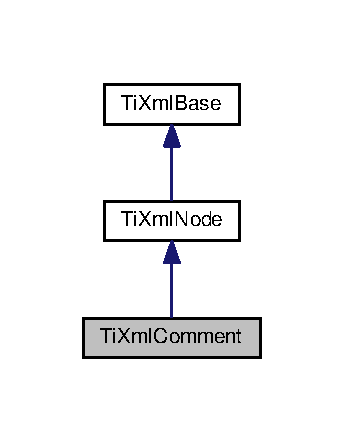
\includegraphics[width=165pt]{classTiXmlComment__inherit__graph}
\end{center}
\end{figure}


Collaboration diagram for Ti\+Xml\+Comment\+:\nopagebreak
\begin{figure}[H]
\begin{center}
\leavevmode
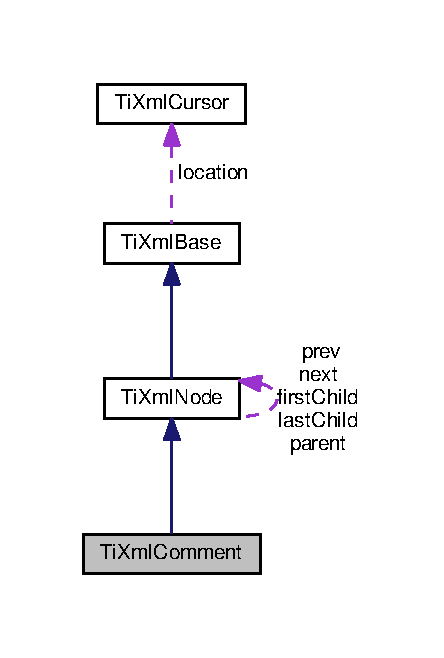
\includegraphics[width=213pt]{classTiXmlComment__coll__graph}
\end{center}
\end{figure}
\subsection*{Public Member Functions}
\begin{DoxyCompactItemize}
\item 
\hyperlink{classTiXmlComment_aaa3252031d3e8bd3a2bf51a1c61201b7}{Ti\+Xml\+Comment} ()\hypertarget{classTiXmlComment_aaa3252031d3e8bd3a2bf51a1c61201b7}{}\label{classTiXmlComment_aaa3252031d3e8bd3a2bf51a1c61201b7}

\begin{DoxyCompactList}\small\item\em Constructs an empty comment. \end{DoxyCompactList}\item 
\hyperlink{classTiXmlComment_a37e7802ef17bc03ebe5ae79bf0713d47}{Ti\+Xml\+Comment} (const char $\ast$\+\_\+value)\hypertarget{classTiXmlComment_a37e7802ef17bc03ebe5ae79bf0713d47}{}\label{classTiXmlComment_a37e7802ef17bc03ebe5ae79bf0713d47}

\begin{DoxyCompactList}\small\item\em Construct a comment from text. \end{DoxyCompactList}\item 
{\bfseries Ti\+Xml\+Comment} (const \hyperlink{classTiXmlComment}{Ti\+Xml\+Comment} \&)\hypertarget{classTiXmlComment_afaec41ac2760ce946ba1590eb5708e50}{}\label{classTiXmlComment_afaec41ac2760ce946ba1590eb5708e50}

\item 
\hyperlink{classTiXmlComment}{Ti\+Xml\+Comment} \& {\bfseries operator=} (const \hyperlink{classTiXmlComment}{Ti\+Xml\+Comment} \&base)\hypertarget{classTiXmlComment_aeceedc15f8b8f9ca0b6136696339b3ac}{}\label{classTiXmlComment_aeceedc15f8b8f9ca0b6136696339b3ac}

\item 
virtual \hyperlink{classTiXmlNode}{Ti\+Xml\+Node} $\ast$ \hyperlink{classTiXmlComment_a4f6590c9c9a2b63a48972655b78eb853}{Clone} () const \hypertarget{classTiXmlComment_a4f6590c9c9a2b63a48972655b78eb853}{}\label{classTiXmlComment_a4f6590c9c9a2b63a48972655b78eb853}

\begin{DoxyCompactList}\small\item\em Returns a copy of this Comment. \end{DoxyCompactList}\item 
virtual void \hyperlink{classTiXmlComment_a17398061d62c470f57801ce28fa33ad4}{Print} (F\+I\+LE $\ast$cfile, int depth) const 
\item 
virtual const char $\ast$ {\bfseries Parse} (const char $\ast$p, \hyperlink{classTiXmlParsingData}{Ti\+Xml\+Parsing\+Data} $\ast$data, Ti\+Xml\+Encoding encoding)\hypertarget{classTiXmlComment_a43bddc18ac057734b41d84653b71d3e0}{}\label{classTiXmlComment_a43bddc18ac057734b41d84653b71d3e0}

\item 
virtual const \hyperlink{classTiXmlComment}{Ti\+Xml\+Comment} $\ast$ \hyperlink{classTiXmlComment_a00fb4215c20a2399ea05ac9b9e7e68a0}{To\+Comment} () const \hypertarget{classTiXmlComment_a00fb4215c20a2399ea05ac9b9e7e68a0}{}\label{classTiXmlComment_a00fb4215c20a2399ea05ac9b9e7e68a0}

\begin{DoxyCompactList}\small\item\em Cast to a more defined type. Will return null not of the requested type. \end{DoxyCompactList}\item 
virtual \hyperlink{classTiXmlComment}{Ti\+Xml\+Comment} $\ast$ \hyperlink{classTiXmlComment_acc7c7e07e13c23f17797d642981511df}{To\+Comment} ()\hypertarget{classTiXmlComment_acc7c7e07e13c23f17797d642981511df}{}\label{classTiXmlComment_acc7c7e07e13c23f17797d642981511df}

\begin{DoxyCompactList}\small\item\em Cast to a more defined type. Will return null not of the requested type. \end{DoxyCompactList}\item 
virtual bool \hyperlink{classTiXmlComment_a4382de0e50da973f11a23ea5852568bd}{Accept} (\hyperlink{classTiXmlVisitor}{Ti\+Xml\+Visitor} $\ast$visitor) const 
\end{DoxyCompactItemize}
\subsection*{Protected Member Functions}
\begin{DoxyCompactItemize}
\item 
void {\bfseries Copy\+To} (\hyperlink{classTiXmlComment}{Ti\+Xml\+Comment} $\ast$target) const \hypertarget{classTiXmlComment_a3175b2f27628f4fb7a043897930cd934}{}\label{classTiXmlComment_a3175b2f27628f4fb7a043897930cd934}

\end{DoxyCompactItemize}
\subsection*{Additional Inherited Members}


\subsection{Detailed Description}
An X\+ML comment. 

\subsection{Member Function Documentation}
\index{Ti\+Xml\+Comment@{Ti\+Xml\+Comment}!Accept@{Accept}}
\index{Accept@{Accept}!Ti\+Xml\+Comment@{Ti\+Xml\+Comment}}
\subsubsection[{\texorpdfstring{Accept(\+Ti\+Xml\+Visitor $\ast$visitor) const }{Accept(TiXmlVisitor *visitor) const }}]{\setlength{\rightskip}{0pt plus 5cm}bool Ti\+Xml\+Comment\+::\+Accept (
\begin{DoxyParamCaption}
\item[{{\bf Ti\+Xml\+Visitor} $\ast$}]{visitor}
\end{DoxyParamCaption}
) const\hspace{0.3cm}{\ttfamily [virtual]}}\hypertarget{classTiXmlComment_a4382de0e50da973f11a23ea5852568bd}{}\label{classTiXmlComment_a4382de0e50da973f11a23ea5852568bd}
Walk the X\+ML tree visiting this node and all of its children. 

Implements \hyperlink{classTiXmlNode_acc0f88b7462c6cb73809d410a4f5bb86}{Ti\+Xml\+Node}.

\index{Ti\+Xml\+Comment@{Ti\+Xml\+Comment}!Print@{Print}}
\index{Print@{Print}!Ti\+Xml\+Comment@{Ti\+Xml\+Comment}}
\subsubsection[{\texorpdfstring{Print(\+F\+I\+L\+E $\ast$cfile, int depth) const }{Print(FILE *cfile, int depth) const }}]{\setlength{\rightskip}{0pt plus 5cm}void Ti\+Xml\+Comment\+::\+Print (
\begin{DoxyParamCaption}
\item[{F\+I\+LE $\ast$}]{cfile, }
\item[{int}]{depth}
\end{DoxyParamCaption}
) const\hspace{0.3cm}{\ttfamily [virtual]}}\hypertarget{classTiXmlComment_a17398061d62c470f57801ce28fa33ad4}{}\label{classTiXmlComment_a17398061d62c470f57801ce28fa33ad4}
All Tiny\+Xml classes can print themselves to a filestream or the string class (\hyperlink{classTiXmlString}{Ti\+Xml\+String} in non-\/\+S\+TL mode, std\+::string in S\+TL mode.) Either or both cfile and str can be null.

This is a formatted print, and will insert tabs and newlines.

(For an unformatted stream, use the $<$$<$ operator.) 

Implements \hyperlink{classTiXmlBase_a0de56b3f2ef14c65091a3b916437b512}{Ti\+Xml\+Base}.



The documentation for this class was generated from the following files\+:\begin{DoxyCompactItemize}
\item 
src/tinyxml/tinyxml.\+h\item 
src/tinyxml/tinyxml.\+cpp\item 
src/tinyxml/tinyxmlparser.\+cpp\end{DoxyCompactItemize}

\hypertarget{structTiXmlCursor}{}\section{Ti\+Xml\+Cursor Struct Reference}
\label{structTiXmlCursor}\index{Ti\+Xml\+Cursor@{Ti\+Xml\+Cursor}}
\subsection*{Public Member Functions}
\begin{DoxyCompactItemize}
\item 
void {\bfseries Clear} ()\hypertarget{structTiXmlCursor_a1e6fa622b59dafb71b6efe595105dcdd}{}\label{structTiXmlCursor_a1e6fa622b59dafb71b6efe595105dcdd}

\end{DoxyCompactItemize}
\subsection*{Public Attributes}
\begin{DoxyCompactItemize}
\item 
int {\bfseries row}\hypertarget{structTiXmlCursor_a5b54dd949820c2db061e2be41f3effb3}{}\label{structTiXmlCursor_a5b54dd949820c2db061e2be41f3effb3}

\item 
int {\bfseries col}\hypertarget{structTiXmlCursor_a5694d7ed2c4d20109d350c14c417969d}{}\label{structTiXmlCursor_a5694d7ed2c4d20109d350c14c417969d}

\end{DoxyCompactItemize}


The documentation for this struct was generated from the following file\+:\begin{DoxyCompactItemize}
\item 
src/tinyxml/tinyxml.\+h\end{DoxyCompactItemize}

\hypertarget{classTiXmlDeclaration}{}\section{Ti\+Xml\+Declaration Class Reference}
\label{classTiXmlDeclaration}\index{Ti\+Xml\+Declaration@{Ti\+Xml\+Declaration}}


{\ttfamily \#include $<$tinyxml.\+h$>$}



Inheritance diagram for Ti\+Xml\+Declaration\+:\nopagebreak
\begin{figure}[H]
\begin{center}
\leavevmode
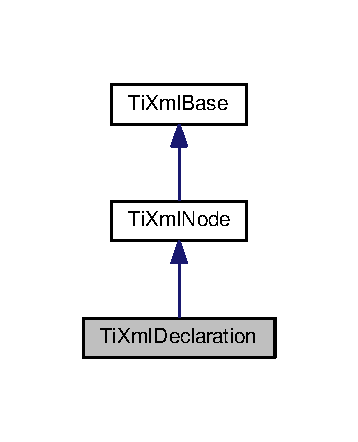
\includegraphics[width=172pt]{classTiXmlDeclaration__inherit__graph}
\end{center}
\end{figure}


Collaboration diagram for Ti\+Xml\+Declaration\+:\nopagebreak
\begin{figure}[H]
\begin{center}
\leavevmode
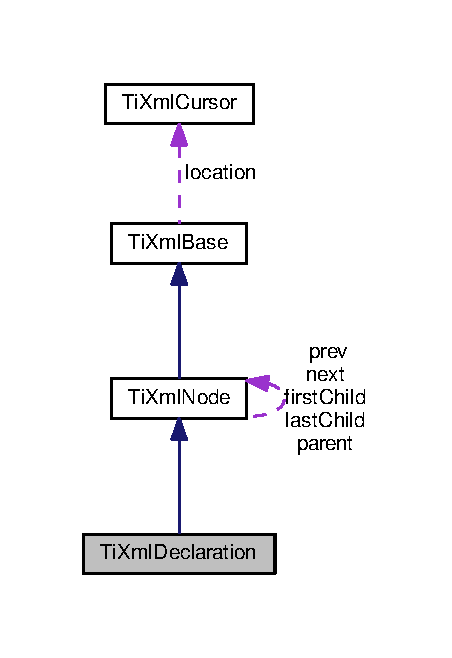
\includegraphics[width=217pt]{classTiXmlDeclaration__coll__graph}
\end{center}
\end{figure}
\subsection*{Public Member Functions}
\begin{DoxyCompactItemize}
\item 
\hyperlink{classTiXmlDeclaration_aa0484d059bea0ea1acb47c9094382d79}{Ti\+Xml\+Declaration} ()\hypertarget{classTiXmlDeclaration_aa0484d059bea0ea1acb47c9094382d79}{}\label{classTiXmlDeclaration_aa0484d059bea0ea1acb47c9094382d79}

\begin{DoxyCompactList}\small\item\em Construct an empty declaration. \end{DoxyCompactList}\item 
\hyperlink{classTiXmlDeclaration_a3b618d1c30c25e4b7a71f31a595ee298}{Ti\+Xml\+Declaration} (const char $\ast$\+\_\+version, const char $\ast$\+\_\+encoding, const char $\ast$\+\_\+standalone)\hypertarget{classTiXmlDeclaration_a3b618d1c30c25e4b7a71f31a595ee298}{}\label{classTiXmlDeclaration_a3b618d1c30c25e4b7a71f31a595ee298}

\begin{DoxyCompactList}\small\item\em Construct. \end{DoxyCompactList}\item 
{\bfseries Ti\+Xml\+Declaration} (const \hyperlink{classTiXmlDeclaration}{Ti\+Xml\+Declaration} \&copy)\hypertarget{classTiXmlDeclaration_a58ac9042c342f7845c8491da0bb091e8}{}\label{classTiXmlDeclaration_a58ac9042c342f7845c8491da0bb091e8}

\item 
\hyperlink{classTiXmlDeclaration}{Ti\+Xml\+Declaration} \& {\bfseries operator=} (const \hyperlink{classTiXmlDeclaration}{Ti\+Xml\+Declaration} \&copy)\hypertarget{classTiXmlDeclaration_a3bc617efe11014ff2b1a9c5727c37a9a}{}\label{classTiXmlDeclaration_a3bc617efe11014ff2b1a9c5727c37a9a}

\item 
const char $\ast$ \hyperlink{classTiXmlDeclaration_a02ee557b1a4545c3219ed377c103ec76}{Version} () const \hypertarget{classTiXmlDeclaration_a02ee557b1a4545c3219ed377c103ec76}{}\label{classTiXmlDeclaration_a02ee557b1a4545c3219ed377c103ec76}

\begin{DoxyCompactList}\small\item\em Version. Will return an empty string if none was found. \end{DoxyCompactList}\item 
const char $\ast$ \hyperlink{classTiXmlDeclaration_a5d974231f9e9a2f0542f15f3a46cdb76}{Encoding} () const \hypertarget{classTiXmlDeclaration_a5d974231f9e9a2f0542f15f3a46cdb76}{}\label{classTiXmlDeclaration_a5d974231f9e9a2f0542f15f3a46cdb76}

\begin{DoxyCompactList}\small\item\em Encoding. Will return an empty string if none was found. \end{DoxyCompactList}\item 
const char $\ast$ \hyperlink{classTiXmlDeclaration_a9ff06afc033d7ef730ec7c6825b97ad9}{Standalone} () const \hypertarget{classTiXmlDeclaration_a9ff06afc033d7ef730ec7c6825b97ad9}{}\label{classTiXmlDeclaration_a9ff06afc033d7ef730ec7c6825b97ad9}

\begin{DoxyCompactList}\small\item\em Is this a standalone document? \end{DoxyCompactList}\item 
virtual \hyperlink{classTiXmlNode}{Ti\+Xml\+Node} $\ast$ \hyperlink{classTiXmlDeclaration_aff8231266d735943d8a7514a9c9822b9}{Clone} () const \hypertarget{classTiXmlDeclaration_aff8231266d735943d8a7514a9c9822b9}{}\label{classTiXmlDeclaration_aff8231266d735943d8a7514a9c9822b9}

\begin{DoxyCompactList}\small\item\em Creates a copy of this Declaration and returns it. \end{DoxyCompactList}\item 
virtual void {\bfseries Print} (F\+I\+LE $\ast$cfile, int depth, T\+I\+X\+M\+L\+\_\+\+S\+T\+R\+I\+NG $\ast$str) const \hypertarget{classTiXmlDeclaration_aa5ab32ec19d4eeecff4a9238c6c90565}{}\label{classTiXmlDeclaration_aa5ab32ec19d4eeecff4a9238c6c90565}

\item 
virtual void \hyperlink{classTiXmlDeclaration_abf6303db4bd05b5be554036817ff1cb4}{Print} (F\+I\+LE $\ast$cfile, int depth) const 
\item 
virtual const char $\ast$ {\bfseries Parse} (const char $\ast$p, \hyperlink{classTiXmlParsingData}{Ti\+Xml\+Parsing\+Data} $\ast$data, Ti\+Xml\+Encoding encoding)\hypertarget{classTiXmlDeclaration_a9839ea97ed687a2b7342fd7b0f04361b}{}\label{classTiXmlDeclaration_a9839ea97ed687a2b7342fd7b0f04361b}

\item 
virtual const \hyperlink{classTiXmlDeclaration}{Ti\+Xml\+Declaration} $\ast$ \hyperlink{classTiXmlDeclaration_a1e085d3fefd1dbf5ccdbff729931a967}{To\+Declaration} () const \hypertarget{classTiXmlDeclaration_a1e085d3fefd1dbf5ccdbff729931a967}{}\label{classTiXmlDeclaration_a1e085d3fefd1dbf5ccdbff729931a967}

\begin{DoxyCompactList}\small\item\em Cast to a more defined type. Will return null not of the requested type. \end{DoxyCompactList}\item 
virtual \hyperlink{classTiXmlDeclaration}{Ti\+Xml\+Declaration} $\ast$ \hyperlink{classTiXmlDeclaration_a6bd3d1daddcaeb9543c24bfd090969ce}{To\+Declaration} ()\hypertarget{classTiXmlDeclaration_a6bd3d1daddcaeb9543c24bfd090969ce}{}\label{classTiXmlDeclaration_a6bd3d1daddcaeb9543c24bfd090969ce}

\begin{DoxyCompactList}\small\item\em Cast to a more defined type. Will return null not of the requested type. \end{DoxyCompactList}\item 
virtual bool \hyperlink{classTiXmlDeclaration_ab6a6b178161ba9abc2c35058de689864}{Accept} (\hyperlink{classTiXmlVisitor}{Ti\+Xml\+Visitor} $\ast$visitor) const 
\end{DoxyCompactItemize}
\subsection*{Protected Member Functions}
\begin{DoxyCompactItemize}
\item 
void {\bfseries Copy\+To} (\hyperlink{classTiXmlDeclaration}{Ti\+Xml\+Declaration} $\ast$target) const \hypertarget{classTiXmlDeclaration_a9d08959f935421a593032bd3efb30c38}{}\label{classTiXmlDeclaration_a9d08959f935421a593032bd3efb30c38}

\end{DoxyCompactItemize}
\subsection*{Additional Inherited Members}


\subsection{Detailed Description}
In correct X\+ML the declaration is the first entry in the file. \begin{DoxyVerb}    <?xml version="1.0" standalone="yes"?>
\end{DoxyVerb}


Tiny\+Xml will happily read or write files without a declaration, however. There are 3 possible attributes to the declaration\+: version, encoding, and standalone.

Note\+: In this version of the code, the attributes are handled as special cases, not generic attributes, simply because there can only be at most 3 and they are always the same. 

\subsection{Member Function Documentation}
\index{Ti\+Xml\+Declaration@{Ti\+Xml\+Declaration}!Accept@{Accept}}
\index{Accept@{Accept}!Ti\+Xml\+Declaration@{Ti\+Xml\+Declaration}}
\subsubsection[{\texorpdfstring{Accept(\+Ti\+Xml\+Visitor $\ast$visitor) const }{Accept(TiXmlVisitor *visitor) const }}]{\setlength{\rightskip}{0pt plus 5cm}bool Ti\+Xml\+Declaration\+::\+Accept (
\begin{DoxyParamCaption}
\item[{{\bf Ti\+Xml\+Visitor} $\ast$}]{visitor}
\end{DoxyParamCaption}
) const\hspace{0.3cm}{\ttfamily [virtual]}}\hypertarget{classTiXmlDeclaration_ab6a6b178161ba9abc2c35058de689864}{}\label{classTiXmlDeclaration_ab6a6b178161ba9abc2c35058de689864}
Walk the X\+ML tree visiting this node and all of its children. 

Implements \hyperlink{classTiXmlNode_acc0f88b7462c6cb73809d410a4f5bb86}{Ti\+Xml\+Node}.

\index{Ti\+Xml\+Declaration@{Ti\+Xml\+Declaration}!Print@{Print}}
\index{Print@{Print}!Ti\+Xml\+Declaration@{Ti\+Xml\+Declaration}}
\subsubsection[{\texorpdfstring{Print(\+F\+I\+L\+E $\ast$cfile, int depth) const }{Print(FILE *cfile, int depth) const }}]{\setlength{\rightskip}{0pt plus 5cm}virtual void Ti\+Xml\+Declaration\+::\+Print (
\begin{DoxyParamCaption}
\item[{F\+I\+LE $\ast$}]{cfile, }
\item[{int}]{depth}
\end{DoxyParamCaption}
) const\hspace{0.3cm}{\ttfamily [inline]}, {\ttfamily [virtual]}}\hypertarget{classTiXmlDeclaration_abf6303db4bd05b5be554036817ff1cb4}{}\label{classTiXmlDeclaration_abf6303db4bd05b5be554036817ff1cb4}
All Tiny\+Xml classes can print themselves to a filestream or the string class (\hyperlink{classTiXmlString}{Ti\+Xml\+String} in non-\/\+S\+TL mode, std\+::string in S\+TL mode.) Either or both cfile and str can be null.

This is a formatted print, and will insert tabs and newlines.

(For an unformatted stream, use the $<$$<$ operator.) 

Implements \hyperlink{classTiXmlBase_a0de56b3f2ef14c65091a3b916437b512}{Ti\+Xml\+Base}.



The documentation for this class was generated from the following files\+:\begin{DoxyCompactItemize}
\item 
src/tinyxml/tinyxml.\+h\item 
src/tinyxml/tinyxml.\+cpp\item 
src/tinyxml/tinyxmlparser.\+cpp\end{DoxyCompactItemize}

\hypertarget{classTiXmlDocument}{}\section{Ti\+Xml\+Document Class Reference}
\label{classTiXmlDocument}\index{Ti\+Xml\+Document@{Ti\+Xml\+Document}}


{\ttfamily \#include $<$tinyxml.\+h$>$}



Inheritance diagram for Ti\+Xml\+Document\+:\nopagebreak
\begin{figure}[H]
\begin{center}
\leavevmode
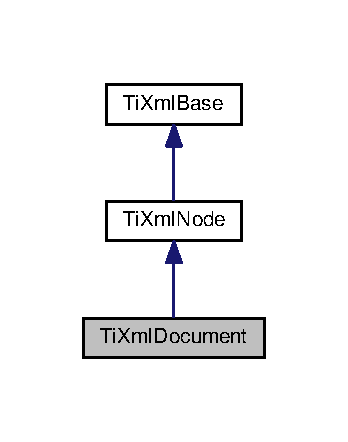
\includegraphics[width=167pt]{classTiXmlDocument__inherit__graph}
\end{center}
\end{figure}


Collaboration diagram for Ti\+Xml\+Document\+:\nopagebreak
\begin{figure}[H]
\begin{center}
\leavevmode
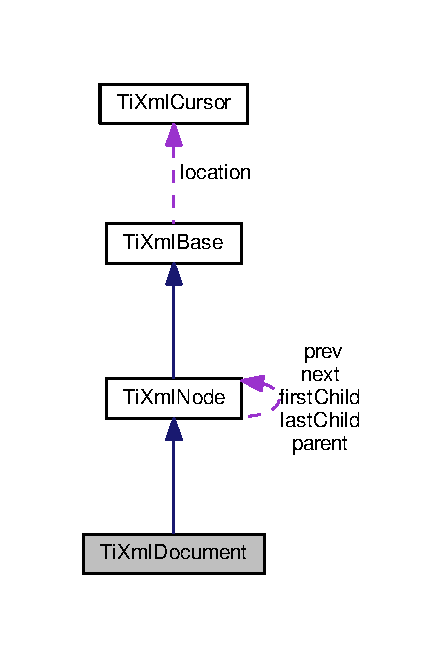
\includegraphics[width=214pt]{classTiXmlDocument__coll__graph}
\end{center}
\end{figure}
\subsection*{Public Member Functions}
\begin{DoxyCompactItemize}
\item 
\hyperlink{classTiXmlDocument_a9f5e84335708fde98400230f9f12659c}{Ti\+Xml\+Document} ()\hypertarget{classTiXmlDocument_a9f5e84335708fde98400230f9f12659c}{}\label{classTiXmlDocument_a9f5e84335708fde98400230f9f12659c}

\begin{DoxyCompactList}\small\item\em Create an empty document, that has no name. \end{DoxyCompactList}\item 
\hyperlink{classTiXmlDocument_ae4508b452d0c3061db085f3db27b8396}{Ti\+Xml\+Document} (const char $\ast$document\+Name)\hypertarget{classTiXmlDocument_ae4508b452d0c3061db085f3db27b8396}{}\label{classTiXmlDocument_ae4508b452d0c3061db085f3db27b8396}

\begin{DoxyCompactList}\small\item\em Create a document with a name. The name of the document is also the filename of the xml. \end{DoxyCompactList}\item 
{\bfseries Ti\+Xml\+Document} (const \hyperlink{classTiXmlDocument}{Ti\+Xml\+Document} \&copy)\hypertarget{classTiXmlDocument_a323a7486e7da6099cdc19a5ff7e74b07}{}\label{classTiXmlDocument_a323a7486e7da6099cdc19a5ff7e74b07}

\item 
\hyperlink{classTiXmlDocument}{Ti\+Xml\+Document} \& {\bfseries operator=} (const \hyperlink{classTiXmlDocument}{Ti\+Xml\+Document} \&copy)\hypertarget{classTiXmlDocument_aa56fd4dbe8917d2033d865909e2d737e}{}\label{classTiXmlDocument_aa56fd4dbe8917d2033d865909e2d737e}

\item 
bool \hyperlink{classTiXmlDocument_a4c852a889c02cf251117fd1d9fe1845f}{Load\+File} (Ti\+Xml\+Encoding encoding=T\+I\+X\+M\+L\+\_\+\+D\+E\+F\+A\+U\+L\+T\+\_\+\+E\+N\+C\+O\+D\+I\+NG)
\item 
bool \hyperlink{classTiXmlDocument_a21c0aeb0d0a720169ad4ac89523ebe93}{Save\+File} () const \hypertarget{classTiXmlDocument_a21c0aeb0d0a720169ad4ac89523ebe93}{}\label{classTiXmlDocument_a21c0aeb0d0a720169ad4ac89523ebe93}

\begin{DoxyCompactList}\small\item\em Save a file using the current document value. Returns true if successful. \end{DoxyCompactList}\item 
bool \hyperlink{classTiXmlDocument_a879cdf5e981b8b2d2ef82f2546dd28fb}{Load\+File} (const char $\ast$filename, Ti\+Xml\+Encoding encoding=T\+I\+X\+M\+L\+\_\+\+D\+E\+F\+A\+U\+L\+T\+\_\+\+E\+N\+C\+O\+D\+I\+NG)\hypertarget{classTiXmlDocument_a879cdf5e981b8b2d2ef82f2546dd28fb}{}\label{classTiXmlDocument_a879cdf5e981b8b2d2ef82f2546dd28fb}

\begin{DoxyCompactList}\small\item\em Load a file using the given filename. Returns true if successful. \end{DoxyCompactList}\item 
bool \hyperlink{classTiXmlDocument_ae869f5ebf7fc54c4a1d737fb4689fd44}{Save\+File} (const char $\ast$filename) const \hypertarget{classTiXmlDocument_ae869f5ebf7fc54c4a1d737fb4689fd44}{}\label{classTiXmlDocument_ae869f5ebf7fc54c4a1d737fb4689fd44}

\begin{DoxyCompactList}\small\item\em Save a file using the given filename. Returns true if successful. \end{DoxyCompactList}\item 
bool \hyperlink{classTiXmlDocument_a41f6fe7200864d1dca663d230caf8db6}{Load\+File} (F\+I\+LE $\ast$, Ti\+Xml\+Encoding encoding=T\+I\+X\+M\+L\+\_\+\+D\+E\+F\+A\+U\+L\+T\+\_\+\+E\+N\+C\+O\+D\+I\+NG)
\item 
bool \hyperlink{classTiXmlDocument_acf1672b4538c6d1d441f9f108aea2bf4}{Save\+File} (F\+I\+LE $\ast$) const \hypertarget{classTiXmlDocument_acf1672b4538c6d1d441f9f108aea2bf4}{}\label{classTiXmlDocument_acf1672b4538c6d1d441f9f108aea2bf4}

\begin{DoxyCompactList}\small\item\em Save a file using the given F\+I\+L\+E$\ast$. Returns true if successful. \end{DoxyCompactList}\item 
virtual const char $\ast$ \hyperlink{classTiXmlDocument_a789ad2f06f93d52bdb5570b2f3670289}{Parse} (const char $\ast$p, \hyperlink{classTiXmlParsingData}{Ti\+Xml\+Parsing\+Data} $\ast$data=0, Ti\+Xml\+Encoding encoding=T\+I\+X\+M\+L\+\_\+\+D\+E\+F\+A\+U\+L\+T\+\_\+\+E\+N\+C\+O\+D\+I\+NG)
\item 
const \hyperlink{classTiXmlElement}{Ti\+Xml\+Element} $\ast$ \hyperlink{classTiXmlDocument_ad09d17927f908f40efb406af2fb873be}{Root\+Element} () const 
\item 
\hyperlink{classTiXmlElement}{Ti\+Xml\+Element} $\ast$ {\bfseries Root\+Element} ()\hypertarget{classTiXmlDocument_a0b43e762a23f938b06651bc90b8a1013}{}\label{classTiXmlDocument_a0b43e762a23f938b06651bc90b8a1013}

\item 
bool \hyperlink{classTiXmlDocument_a6dfc01a6e5d58e56acd537dfd3bdeb29}{Error} () const 
\item 
const char $\ast$ \hyperlink{classTiXmlDocument_a9d0f689f6e09ea494ea547be8d79c25e}{Error\+Desc} () const \hypertarget{classTiXmlDocument_a9d0f689f6e09ea494ea547be8d79c25e}{}\label{classTiXmlDocument_a9d0f689f6e09ea494ea547be8d79c25e}

\begin{DoxyCompactList}\small\item\em Contains a textual (english) description of the error if one occurs. \end{DoxyCompactList}\item 
int \hyperlink{classTiXmlDocument_af96fc2f3f9ec6422782bfe916c9e778f}{Error\+Id} () const 
\item 
int \hyperlink{classTiXmlDocument_af30efc75e804aa2e92fb8be3a8cb676e}{Error\+Row} () const 
\item 
int \hyperlink{classTiXmlDocument_aa90bc630ee5203c6109ca5fad3323649}{Error\+Col} () const \hypertarget{classTiXmlDocument_aa90bc630ee5203c6109ca5fad3323649}{}\label{classTiXmlDocument_aa90bc630ee5203c6109ca5fad3323649}

\begin{DoxyCompactList}\small\item\em The column where the error occured. See \hyperlink{classTiXmlDocument_af30efc75e804aa2e92fb8be3a8cb676e}{Error\+Row()} \end{DoxyCompactList}\item 
void \hyperlink{classTiXmlDocument_a51dac56316f89b35bdb7d0d433ba988e}{Set\+Tab\+Size} (int \+\_\+tabsize)
\item 
int {\bfseries Tab\+Size} () const \hypertarget{classTiXmlDocument_a612360241b85bad0826b2a9ae9cda561}{}\label{classTiXmlDocument_a612360241b85bad0826b2a9ae9cda561}

\item 
void \hyperlink{classTiXmlDocument_ac66b8c28db86363315712a3574e87c35}{Clear\+Error} ()
\item 
void \hyperlink{classTiXmlDocument_af08389ec70ee9b2de7f800e206a18510}{Print} () const 
\item 
virtual void \hyperlink{classTiXmlDocument_a7b1aea204fee266b70b9c105c8bf2ada}{Print} (F\+I\+LE $\ast$cfile, int depth=0) const \hypertarget{classTiXmlDocument_a7b1aea204fee266b70b9c105c8bf2ada}{}\label{classTiXmlDocument_a7b1aea204fee266b70b9c105c8bf2ada}

\begin{DoxyCompactList}\small\item\em Print this Document to a F\+I\+LE stream. \end{DoxyCompactList}\item 
void {\bfseries Set\+Error} (int err, const char $\ast$error\+Location, \hyperlink{classTiXmlParsingData}{Ti\+Xml\+Parsing\+Data} $\ast$prev\+Data, Ti\+Xml\+Encoding encoding)\hypertarget{classTiXmlDocument_a735c23e318597b920c94eae77fa206de}{}\label{classTiXmlDocument_a735c23e318597b920c94eae77fa206de}

\item 
virtual const \hyperlink{classTiXmlDocument}{Ti\+Xml\+Document} $\ast$ \hyperlink{classTiXmlDocument_a1dc977bde3e4fe85a8eb9d88a35ef5a4}{To\+Document} () const \hypertarget{classTiXmlDocument_a1dc977bde3e4fe85a8eb9d88a35ef5a4}{}\label{classTiXmlDocument_a1dc977bde3e4fe85a8eb9d88a35ef5a4}

\begin{DoxyCompactList}\small\item\em Cast to a more defined type. Will return null not of the requested type. \end{DoxyCompactList}\item 
virtual \hyperlink{classTiXmlDocument}{Ti\+Xml\+Document} $\ast$ \hyperlink{classTiXmlDocument_a1025d942a1f328fd742d545e37efdd42}{To\+Document} ()\hypertarget{classTiXmlDocument_a1025d942a1f328fd742d545e37efdd42}{}\label{classTiXmlDocument_a1025d942a1f328fd742d545e37efdd42}

\begin{DoxyCompactList}\small\item\em Cast to a more defined type. Will return null not of the requested type. \end{DoxyCompactList}\item 
virtual bool \hyperlink{classTiXmlDocument_a3daab2f472418ef66315750202f762ae}{Accept} (\hyperlink{classTiXmlVisitor}{Ti\+Xml\+Visitor} $\ast$content) const 
\end{DoxyCompactItemize}
\subsection*{Protected Member Functions}
\begin{DoxyCompactItemize}
\item 
virtual \hyperlink{classTiXmlNode}{Ti\+Xml\+Node} $\ast$ \hyperlink{classTiXmlDocument_ac9e8f09b23454d953b32d1b65cd1409e}{Clone} () const 
\end{DoxyCompactItemize}
\subsection*{Additional Inherited Members}


\subsection{Detailed Description}
Always the top level node. A document binds together all the X\+ML pieces. It can be saved, loaded, and printed to the screen. The \textquotesingle{}value\textquotesingle{} of a document node is the xml file name. 

\subsection{Member Function Documentation}
\index{Ti\+Xml\+Document@{Ti\+Xml\+Document}!Accept@{Accept}}
\index{Accept@{Accept}!Ti\+Xml\+Document@{Ti\+Xml\+Document}}
\subsubsection[{\texorpdfstring{Accept(\+Ti\+Xml\+Visitor $\ast$content) const }{Accept(TiXmlVisitor *content) const }}]{\setlength{\rightskip}{0pt plus 5cm}bool Ti\+Xml\+Document\+::\+Accept (
\begin{DoxyParamCaption}
\item[{{\bf Ti\+Xml\+Visitor} $\ast$}]{content}
\end{DoxyParamCaption}
) const\hspace{0.3cm}{\ttfamily [virtual]}}\hypertarget{classTiXmlDocument_a3daab2f472418ef66315750202f762ae}{}\label{classTiXmlDocument_a3daab2f472418ef66315750202f762ae}
Walk the X\+ML tree visiting this node and all of its children. 

Implements \hyperlink{classTiXmlNode_acc0f88b7462c6cb73809d410a4f5bb86}{Ti\+Xml\+Node}.

\index{Ti\+Xml\+Document@{Ti\+Xml\+Document}!Clear\+Error@{Clear\+Error}}
\index{Clear\+Error@{Clear\+Error}!Ti\+Xml\+Document@{Ti\+Xml\+Document}}
\subsubsection[{\texorpdfstring{Clear\+Error()}{ClearError()}}]{\setlength{\rightskip}{0pt plus 5cm}void Ti\+Xml\+Document\+::\+Clear\+Error (
\begin{DoxyParamCaption}
{}
\end{DoxyParamCaption}
)\hspace{0.3cm}{\ttfamily [inline]}}\hypertarget{classTiXmlDocument_ac66b8c28db86363315712a3574e87c35}{}\label{classTiXmlDocument_ac66b8c28db86363315712a3574e87c35}
If you have handled the error, it can be reset with this call. The error state is automatically cleared if you Parse a new X\+ML block. \index{Ti\+Xml\+Document@{Ti\+Xml\+Document}!Clone@{Clone}}
\index{Clone@{Clone}!Ti\+Xml\+Document@{Ti\+Xml\+Document}}
\subsubsection[{\texorpdfstring{Clone() const }{Clone() const }}]{\setlength{\rightskip}{0pt plus 5cm}{\bf Ti\+Xml\+Node} $\ast$ Ti\+Xml\+Document\+::\+Clone (
\begin{DoxyParamCaption}
{}
\end{DoxyParamCaption}
) const\hspace{0.3cm}{\ttfamily [protected]}, {\ttfamily [virtual]}}\hypertarget{classTiXmlDocument_ac9e8f09b23454d953b32d1b65cd1409e}{}\label{classTiXmlDocument_ac9e8f09b23454d953b32d1b65cd1409e}
Create an exact duplicate of this node and return it. The memory must be deleted by the caller. 

Implements \hyperlink{classTiXmlNode_a4508cc3a2d7a98e96a54cc09c37a78a4}{Ti\+Xml\+Node}.

\index{Ti\+Xml\+Document@{Ti\+Xml\+Document}!Error@{Error}}
\index{Error@{Error}!Ti\+Xml\+Document@{Ti\+Xml\+Document}}
\subsubsection[{\texorpdfstring{Error() const }{Error() const }}]{\setlength{\rightskip}{0pt plus 5cm}bool Ti\+Xml\+Document\+::\+Error (
\begin{DoxyParamCaption}
{}
\end{DoxyParamCaption}
) const\hspace{0.3cm}{\ttfamily [inline]}}\hypertarget{classTiXmlDocument_a6dfc01a6e5d58e56acd537dfd3bdeb29}{}\label{classTiXmlDocument_a6dfc01a6e5d58e56acd537dfd3bdeb29}
If an error occurs, Error will be set to true. Also,
\begin{DoxyItemize}
\item The \hyperlink{classTiXmlDocument_af96fc2f3f9ec6422782bfe916c9e778f}{Error\+Id()} will contain the integer identifier of the error (not generally useful)
\item The \hyperlink{classTiXmlDocument_a9d0f689f6e09ea494ea547be8d79c25e}{Error\+Desc()} method will return the name of the error. (very useful)
\item The \hyperlink{classTiXmlDocument_af30efc75e804aa2e92fb8be3a8cb676e}{Error\+Row()} and \hyperlink{classTiXmlDocument_aa90bc630ee5203c6109ca5fad3323649}{Error\+Col()} will return the location of the error (if known) 
\end{DoxyItemize}\index{Ti\+Xml\+Document@{Ti\+Xml\+Document}!Error\+Id@{Error\+Id}}
\index{Error\+Id@{Error\+Id}!Ti\+Xml\+Document@{Ti\+Xml\+Document}}
\subsubsection[{\texorpdfstring{Error\+Id() const }{ErrorId() const }}]{\setlength{\rightskip}{0pt plus 5cm}int Ti\+Xml\+Document\+::\+Error\+Id (
\begin{DoxyParamCaption}
{}
\end{DoxyParamCaption}
) const\hspace{0.3cm}{\ttfamily [inline]}}\hypertarget{classTiXmlDocument_af96fc2f3f9ec6422782bfe916c9e778f}{}\label{classTiXmlDocument_af96fc2f3f9ec6422782bfe916c9e778f}
Generally, you probably want the error string ( \hyperlink{classTiXmlDocument_a9d0f689f6e09ea494ea547be8d79c25e}{Error\+Desc()} ). But if you prefer the Error\+Id, this function will fetch it. \index{Ti\+Xml\+Document@{Ti\+Xml\+Document}!Error\+Row@{Error\+Row}}
\index{Error\+Row@{Error\+Row}!Ti\+Xml\+Document@{Ti\+Xml\+Document}}
\subsubsection[{\texorpdfstring{Error\+Row() const }{ErrorRow() const }}]{\setlength{\rightskip}{0pt plus 5cm}int Ti\+Xml\+Document\+::\+Error\+Row (
\begin{DoxyParamCaption}
{}
\end{DoxyParamCaption}
) const\hspace{0.3cm}{\ttfamily [inline]}}\hypertarget{classTiXmlDocument_af30efc75e804aa2e92fb8be3a8cb676e}{}\label{classTiXmlDocument_af30efc75e804aa2e92fb8be3a8cb676e}
Returns the location (if known) of the error. The first column is column 1, and the first row is row 1. A value of 0 means the row and column wasn\textquotesingle{}t applicable (memory errors, for example, have no row/column) or the parser lost the error. (An error in the error reporting, in that case.)

\begin{DoxySeeAlso}{See also}
\hyperlink{classTiXmlDocument_a51dac56316f89b35bdb7d0d433ba988e}{Set\+Tab\+Size}, \hyperlink{classTiXmlBase_a024bceb070188df92c2a8d8852dd0853}{Row}, \hyperlink{classTiXmlBase_ab54bfb9b70fe6dd276e7b279cab7f003}{Column} 
\end{DoxySeeAlso}
\index{Ti\+Xml\+Document@{Ti\+Xml\+Document}!Load\+File@{Load\+File}}
\index{Load\+File@{Load\+File}!Ti\+Xml\+Document@{Ti\+Xml\+Document}}
\subsubsection[{\texorpdfstring{Load\+File(\+Ti\+Xml\+Encoding encoding=\+T\+I\+X\+M\+L\+\_\+\+D\+E\+F\+A\+U\+L\+T\+\_\+\+E\+N\+C\+O\+D\+I\+N\+G)}{LoadFile(TiXmlEncoding encoding=TIXML_DEFAULT_ENCODING)}}]{\setlength{\rightskip}{0pt plus 5cm}bool Ti\+Xml\+Document\+::\+Load\+File (
\begin{DoxyParamCaption}
\item[{Ti\+Xml\+Encoding}]{encoding = {\ttfamily TIXML\+\_\+DEFAULT\+\_\+ENCODING}}
\end{DoxyParamCaption}
)}\hypertarget{classTiXmlDocument_a4c852a889c02cf251117fd1d9fe1845f}{}\label{classTiXmlDocument_a4c852a889c02cf251117fd1d9fe1845f}
Load a file using the current document value. Returns true if successful. Will delete any existing document data before loading. \index{Ti\+Xml\+Document@{Ti\+Xml\+Document}!Load\+File@{Load\+File}}
\index{Load\+File@{Load\+File}!Ti\+Xml\+Document@{Ti\+Xml\+Document}}
\subsubsection[{\texorpdfstring{Load\+File(\+F\+I\+L\+E $\ast$, Ti\+Xml\+Encoding encoding=\+T\+I\+X\+M\+L\+\_\+\+D\+E\+F\+A\+U\+L\+T\+\_\+\+E\+N\+C\+O\+D\+I\+N\+G)}{LoadFile(FILE *, TiXmlEncoding encoding=TIXML_DEFAULT_ENCODING)}}]{\setlength{\rightskip}{0pt plus 5cm}bool Ti\+Xml\+Document\+::\+Load\+File (
\begin{DoxyParamCaption}
\item[{F\+I\+LE $\ast$}]{file, }
\item[{Ti\+Xml\+Encoding}]{encoding = {\ttfamily TIXML\+\_\+DEFAULT\+\_\+ENCODING}}
\end{DoxyParamCaption}
)}\hypertarget{classTiXmlDocument_a41f6fe7200864d1dca663d230caf8db6}{}\label{classTiXmlDocument_a41f6fe7200864d1dca663d230caf8db6}
Load a file using the given F\+I\+L\+E$\ast$. Returns true if successful. Note that this method doesn\textquotesingle{}t stream -\/ the entire object pointed at by the F\+I\+L\+E$\ast$ will be interpreted as an X\+ML file. Tiny\+X\+ML doesn\textquotesingle{}t stream in X\+ML from the current file location. Streaming may be added in the future. \index{Ti\+Xml\+Document@{Ti\+Xml\+Document}!Parse@{Parse}}
\index{Parse@{Parse}!Ti\+Xml\+Document@{Ti\+Xml\+Document}}
\subsubsection[{\texorpdfstring{Parse(const char $\ast$p, Ti\+Xml\+Parsing\+Data $\ast$data=0, Ti\+Xml\+Encoding encoding=\+T\+I\+X\+M\+L\+\_\+\+D\+E\+F\+A\+U\+L\+T\+\_\+\+E\+N\+C\+O\+D\+I\+N\+G)}{Parse(const char *p, TiXmlParsingData *data=0, TiXmlEncoding encoding=TIXML_DEFAULT_ENCODING)}}]{\setlength{\rightskip}{0pt plus 5cm}const char $\ast$ Ti\+Xml\+Document\+::\+Parse (
\begin{DoxyParamCaption}
\item[{const char $\ast$}]{p, }
\item[{{\bf Ti\+Xml\+Parsing\+Data} $\ast$}]{data = {\ttfamily 0}, }
\item[{Ti\+Xml\+Encoding}]{encoding = {\ttfamily TIXML\+\_\+DEFAULT\+\_\+ENCODING}}
\end{DoxyParamCaption}
)\hspace{0.3cm}{\ttfamily [virtual]}}\hypertarget{classTiXmlDocument_a789ad2f06f93d52bdb5570b2f3670289}{}\label{classTiXmlDocument_a789ad2f06f93d52bdb5570b2f3670289}
Parse the given null terminated block of xml data. Passing in an encoding to this method (either T\+I\+X\+M\+L\+\_\+\+E\+N\+C\+O\+D\+I\+N\+G\+\_\+\+L\+E\+G\+A\+CY or T\+I\+X\+M\+L\+\_\+\+E\+N\+C\+O\+D\+I\+N\+G\+\_\+\+U\+T\+F8 will force Tiny\+Xml to use that encoding, regardless of what Tiny\+Xml might otherwise try to detect. 

Implements \hyperlink{classTiXmlBase}{Ti\+Xml\+Base}.

\index{Ti\+Xml\+Document@{Ti\+Xml\+Document}!Print@{Print}}
\index{Print@{Print}!Ti\+Xml\+Document@{Ti\+Xml\+Document}}
\subsubsection[{\texorpdfstring{Print() const }{Print() const }}]{\setlength{\rightskip}{0pt plus 5cm}void Ti\+Xml\+Document\+::\+Print (
\begin{DoxyParamCaption}
{}
\end{DoxyParamCaption}
) const\hspace{0.3cm}{\ttfamily [inline]}}\hypertarget{classTiXmlDocument_af08389ec70ee9b2de7f800e206a18510}{}\label{classTiXmlDocument_af08389ec70ee9b2de7f800e206a18510}
Write the document to standard out using formatted printing (\char`\"{}pretty print\char`\"{}). \index{Ti\+Xml\+Document@{Ti\+Xml\+Document}!Root\+Element@{Root\+Element}}
\index{Root\+Element@{Root\+Element}!Ti\+Xml\+Document@{Ti\+Xml\+Document}}
\subsubsection[{\texorpdfstring{Root\+Element() const }{RootElement() const }}]{\setlength{\rightskip}{0pt plus 5cm}const {\bf Ti\+Xml\+Element}$\ast$ Ti\+Xml\+Document\+::\+Root\+Element (
\begin{DoxyParamCaption}
{}
\end{DoxyParamCaption}
) const\hspace{0.3cm}{\ttfamily [inline]}}\hypertarget{classTiXmlDocument_ad09d17927f908f40efb406af2fb873be}{}\label{classTiXmlDocument_ad09d17927f908f40efb406af2fb873be}
Get the root element -- the only top level element -- of the document. In well formed X\+ML, there should only be one. Tiny\+Xml is tolerant of multiple elements at the document level. \index{Ti\+Xml\+Document@{Ti\+Xml\+Document}!Set\+Tab\+Size@{Set\+Tab\+Size}}
\index{Set\+Tab\+Size@{Set\+Tab\+Size}!Ti\+Xml\+Document@{Ti\+Xml\+Document}}
\subsubsection[{\texorpdfstring{Set\+Tab\+Size(int \+\_\+tabsize)}{SetTabSize(int _tabsize)}}]{\setlength{\rightskip}{0pt plus 5cm}void Ti\+Xml\+Document\+::\+Set\+Tab\+Size (
\begin{DoxyParamCaption}
\item[{int}]{\+\_\+tabsize}
\end{DoxyParamCaption}
)\hspace{0.3cm}{\ttfamily [inline]}}\hypertarget{classTiXmlDocument_a51dac56316f89b35bdb7d0d433ba988e}{}\label{classTiXmlDocument_a51dac56316f89b35bdb7d0d433ba988e}
\hyperlink{classTiXmlDocument_a51dac56316f89b35bdb7d0d433ba988e}{Set\+Tab\+Size()} allows the error reporting functions (\hyperlink{classTiXmlDocument_af30efc75e804aa2e92fb8be3a8cb676e}{Error\+Row()} and \hyperlink{classTiXmlDocument_aa90bc630ee5203c6109ca5fad3323649}{Error\+Col()}) to report the correct values for row and column. It does not change the output or input in any way.

By calling this method, with a tab size greater than 0, the row and column of each node and attribute is stored when the file is loaded. Very useful for tracking the D\+OM back in to the source file.

The tab size is required for calculating the location of nodes. If not set, the default of 4 is used. The tabsize is set per document. Setting the tabsize to 0 disables row/column tracking.

Note that row and column tracking is not supported when using operator$>$$>$.

The tab size needs to be enabled before the parse or load. Correct usage\+: \begin{DoxyVerb}TiXmlDocument doc;
doc.SetTabSize( 8 );
doc.Load( "myfile.xml" );
\end{DoxyVerb}


\begin{DoxySeeAlso}{See also}
\hyperlink{classTiXmlBase_a024bceb070188df92c2a8d8852dd0853}{Row}, \hyperlink{classTiXmlBase_ab54bfb9b70fe6dd276e7b279cab7f003}{Column} 
\end{DoxySeeAlso}


The documentation for this class was generated from the following files\+:\begin{DoxyCompactItemize}
\item 
src/tinyxml/tinyxml.\+h\item 
src/tinyxml/tinyxml.\+cpp\item 
src/tinyxml/tinyxmlparser.\+cpp\end{DoxyCompactItemize}

\hypertarget{classTiXmlElement}{}\section{Ti\+Xml\+Element Class Reference}
\label{classTiXmlElement}\index{Ti\+Xml\+Element@{Ti\+Xml\+Element}}


{\ttfamily \#include $<$tinyxml.\+h$>$}



Inheritance diagram for Ti\+Xml\+Element\+:\nopagebreak
\begin{figure}[H]
\begin{center}
\leavevmode
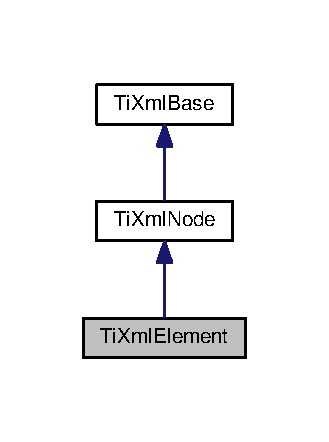
\includegraphics[width=158pt]{classTiXmlElement__inherit__graph}
\end{center}
\end{figure}


Collaboration diagram for Ti\+Xml\+Element\+:\nopagebreak
\begin{figure}[H]
\begin{center}
\leavevmode
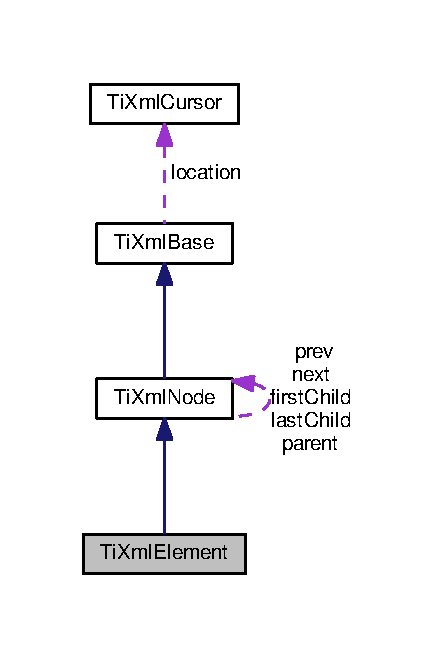
\includegraphics[width=210pt]{classTiXmlElement__coll__graph}
\end{center}
\end{figure}
\subsection*{Public Member Functions}
\begin{DoxyCompactItemize}
\item 
\hyperlink{classTiXmlElement_a01bc3ab372d35da08efcbbe65ad90c60}{Ti\+Xml\+Element} (const char $\ast$in\+\_\+value)\hypertarget{classTiXmlElement_a01bc3ab372d35da08efcbbe65ad90c60}{}\label{classTiXmlElement_a01bc3ab372d35da08efcbbe65ad90c60}

\begin{DoxyCompactList}\small\item\em Construct an element. \end{DoxyCompactList}\item 
{\bfseries Ti\+Xml\+Element} (const \hyperlink{classTiXmlElement}{Ti\+Xml\+Element} \&)\hypertarget{classTiXmlElement_a1ca4465f3c2eac6a60e641cd7f1d9f7e}{}\label{classTiXmlElement_a1ca4465f3c2eac6a60e641cd7f1d9f7e}

\item 
\hyperlink{classTiXmlElement}{Ti\+Xml\+Element} \& {\bfseries operator=} (const \hyperlink{classTiXmlElement}{Ti\+Xml\+Element} \&base)\hypertarget{classTiXmlElement_ad58d300f4cfc0016ffa6861ebb718a0b}{}\label{classTiXmlElement_ad58d300f4cfc0016ffa6861ebb718a0b}

\item 
const char $\ast$ \hyperlink{classTiXmlElement_ac1e4691e9375ba4e665dce7e46a50a9c}{Attribute} (const char $\ast$name) const 
\item 
const char $\ast$ \hyperlink{classTiXmlElement_aa9192e80567b5042dbded80b78c44339}{Attribute} (const char $\ast$name, int $\ast$i) const 
\item 
const char $\ast$ \hyperlink{classTiXmlElement_aec4f727f8aa49b51248d80125d173136}{Attribute} (const char $\ast$name, double $\ast$d) const 
\item 
int \hyperlink{classTiXmlElement_aea0bfe471380f281c5945770ddbf52b9}{Query\+Int\+Attribute} (const char $\ast$name, int $\ast$\+\_\+value) const 
\item 
int \hyperlink{classTiXmlElement_ae48df644f890ab86fa19839ac401f00d}{Query\+Unsigned\+Attribute} (const char $\ast$name, unsigned $\ast$\+\_\+value) const \hypertarget{classTiXmlElement_ae48df644f890ab86fa19839ac401f00d}{}\label{classTiXmlElement_ae48df644f890ab86fa19839ac401f00d}

\begin{DoxyCompactList}\small\item\em Query\+Unsigned\+Attribute examines the attribute -\/ see \hyperlink{classTiXmlElement_aea0bfe471380f281c5945770ddbf52b9}{Query\+Int\+Attribute()}. \end{DoxyCompactList}\item 
int \hyperlink{classTiXmlElement_af4a1d3f88c28eb0f3115dc39ebd83fff}{Query\+Bool\+Attribute} (const char $\ast$name, bool $\ast$\+\_\+value) const 
\item 
int \hyperlink{classTiXmlElement_a898d7730ecc341f0bffc7a9dadbf1ce7}{Query\+Double\+Attribute} (const char $\ast$name, double $\ast$\+\_\+value) const \hypertarget{classTiXmlElement_a898d7730ecc341f0bffc7a9dadbf1ce7}{}\label{classTiXmlElement_a898d7730ecc341f0bffc7a9dadbf1ce7}

\begin{DoxyCompactList}\small\item\em Query\+Double\+Attribute examines the attribute -\/ see \hyperlink{classTiXmlElement_aea0bfe471380f281c5945770ddbf52b9}{Query\+Int\+Attribute()}. \end{DoxyCompactList}\item 
int \hyperlink{classTiXmlElement_aa04d3af11601ef5a5f88295203a843be}{Query\+Float\+Attribute} (const char $\ast$name, float $\ast$\+\_\+value) const \hypertarget{classTiXmlElement_aa04d3af11601ef5a5f88295203a843be}{}\label{classTiXmlElement_aa04d3af11601ef5a5f88295203a843be}

\begin{DoxyCompactList}\small\item\em Query\+Float\+Attribute examines the attribute -\/ see \hyperlink{classTiXmlElement_aea0bfe471380f281c5945770ddbf52b9}{Query\+Int\+Attribute()}. \end{DoxyCompactList}\item 
void \hyperlink{classTiXmlElement_abf0b3bd7f0e4c746a89ec6e7f101fc32}{Set\+Attribute} (const char $\ast$name, const char $\ast$\+\_\+value)
\item 
void \hyperlink{classTiXmlElement_ace6f4be75e373726d4774073d666d1a7}{Set\+Attribute} (const char $\ast$name, int value)
\item 
void \hyperlink{classTiXmlElement_a0d1dd975d75496778177e35abfe0ec0b}{Set\+Double\+Attribute} (const char $\ast$name, double value)
\item 
void \hyperlink{classTiXmlElement_a56979767deca794376b1dfa69a525b2a}{Remove\+Attribute} (const char $\ast$name)
\item 
const \hyperlink{classTiXmlAttribute}{Ti\+Xml\+Attribute} $\ast$ \hyperlink{classTiXmlElement_a516054c9073647d6cb29b6abe9fa0592}{First\+Attribute} () const \hypertarget{classTiXmlElement_a516054c9073647d6cb29b6abe9fa0592}{}\label{classTiXmlElement_a516054c9073647d6cb29b6abe9fa0592}

\begin{DoxyCompactList}\small\item\em Access the first attribute in this element. \end{DoxyCompactList}\item 
\hyperlink{classTiXmlAttribute}{Ti\+Xml\+Attribute} $\ast$ {\bfseries First\+Attribute} ()\hypertarget{classTiXmlElement_a4b33780fc565d38d6b54f640e0cf1737}{}\label{classTiXmlElement_a4b33780fc565d38d6b54f640e0cf1737}

\item 
const \hyperlink{classTiXmlAttribute}{Ti\+Xml\+Attribute} $\ast$ \hyperlink{classTiXmlElement_a86191b49f9177be132b85b14655f1381}{Last\+Attribute} () const \hypertarget{classTiXmlElement_a86191b49f9177be132b85b14655f1381}{}\label{classTiXmlElement_a86191b49f9177be132b85b14655f1381}

\begin{DoxyCompactList}\small\item\em Access the last attribute in this element. \end{DoxyCompactList}\item 
\hyperlink{classTiXmlAttribute}{Ti\+Xml\+Attribute} $\ast$ {\bfseries Last\+Attribute} ()\hypertarget{classTiXmlElement_a222f81cf06155cd108f2a68d4d176004}{}\label{classTiXmlElement_a222f81cf06155cd108f2a68d4d176004}

\item 
const char $\ast$ \hyperlink{classTiXmlElement_aa6dedd8a146acf3b1bc0903deb2d411a}{Get\+Text} () const 
\item 
virtual \hyperlink{classTiXmlNode}{Ti\+Xml\+Node} $\ast$ \hyperlink{classTiXmlElement_a13f6df105ebb1e8dc636e75cc883be32}{Clone} () const \hypertarget{classTiXmlElement_a13f6df105ebb1e8dc636e75cc883be32}{}\label{classTiXmlElement_a13f6df105ebb1e8dc636e75cc883be32}

\begin{DoxyCompactList}\small\item\em Creates a new Element and returns it -\/ the returned element is a copy. \end{DoxyCompactList}\item 
virtual void \hyperlink{classTiXmlElement_ad9d0c008866982ab8d9aafae7e14d692}{Print} (F\+I\+LE $\ast$cfile, int depth) const 
\item 
virtual const char $\ast$ {\bfseries Parse} (const char $\ast$p, \hyperlink{classTiXmlParsingData}{Ti\+Xml\+Parsing\+Data} $\ast$data, Ti\+Xml\+Encoding encoding)\hypertarget{classTiXmlElement_af95c9165159fd9dfdcc5b894a3fcf85b}{}\label{classTiXmlElement_af95c9165159fd9dfdcc5b894a3fcf85b}

\item 
virtual const \hyperlink{classTiXmlElement}{Ti\+Xml\+Element} $\ast$ \hyperlink{classTiXmlElement_ac5b8d0e25fa23fd9acbb6d146082901c}{To\+Element} () const \hypertarget{classTiXmlElement_ac5b8d0e25fa23fd9acbb6d146082901c}{}\label{classTiXmlElement_ac5b8d0e25fa23fd9acbb6d146082901c}

\begin{DoxyCompactList}\small\item\em Cast to a more defined type. Will return null not of the requested type. \end{DoxyCompactList}\item 
virtual \hyperlink{classTiXmlElement}{Ti\+Xml\+Element} $\ast$ \hyperlink{classTiXmlElement_a9def86337ea7a755eb41cac980f60c7a}{To\+Element} ()\hypertarget{classTiXmlElement_a9def86337ea7a755eb41cac980f60c7a}{}\label{classTiXmlElement_a9def86337ea7a755eb41cac980f60c7a}

\begin{DoxyCompactList}\small\item\em Cast to a more defined type. Will return null not of the requested type. \end{DoxyCompactList}\item 
virtual bool \hyperlink{classTiXmlElement_a31ab28cc3b892a69254391d6bbe08df3}{Accept} (\hyperlink{classTiXmlVisitor}{Ti\+Xml\+Visitor} $\ast$visitor) const 
\end{DoxyCompactItemize}
\subsection*{Protected Member Functions}
\begin{DoxyCompactItemize}
\item 
void {\bfseries Copy\+To} (\hyperlink{classTiXmlElement}{Ti\+Xml\+Element} $\ast$target) const \hypertarget{classTiXmlElement_a9e0c1983b840de4134f1f6bf7af00b0f}{}\label{classTiXmlElement_a9e0c1983b840de4134f1f6bf7af00b0f}

\item 
void {\bfseries Clear\+This} ()\hypertarget{classTiXmlElement_a5670933ec2d7d9763b9891acc05d7f7d}{}\label{classTiXmlElement_a5670933ec2d7d9763b9891acc05d7f7d}

\item 
const char $\ast$ {\bfseries Read\+Value} (const char $\ast$in, \hyperlink{classTiXmlParsingData}{Ti\+Xml\+Parsing\+Data} $\ast$prev\+Data, Ti\+Xml\+Encoding encoding)\hypertarget{classTiXmlElement_ac786bce103042d3837c4cc2ff6967d41}{}\label{classTiXmlElement_ac786bce103042d3837c4cc2ff6967d41}

\end{DoxyCompactItemize}
\subsection*{Additional Inherited Members}


\subsection{Detailed Description}
The element is a container class. It has a value, the element name, and can contain other elements, text, comments, and unknowns. Elements also contain an arbitrary number of attributes. 

\subsection{Member Function Documentation}
\index{Ti\+Xml\+Element@{Ti\+Xml\+Element}!Accept@{Accept}}
\index{Accept@{Accept}!Ti\+Xml\+Element@{Ti\+Xml\+Element}}
\subsubsection[{\texorpdfstring{Accept(\+Ti\+Xml\+Visitor $\ast$visitor) const }{Accept(TiXmlVisitor *visitor) const }}]{\setlength{\rightskip}{0pt plus 5cm}bool Ti\+Xml\+Element\+::\+Accept (
\begin{DoxyParamCaption}
\item[{{\bf Ti\+Xml\+Visitor} $\ast$}]{visitor}
\end{DoxyParamCaption}
) const\hspace{0.3cm}{\ttfamily [virtual]}}\hypertarget{classTiXmlElement_a31ab28cc3b892a69254391d6bbe08df3}{}\label{classTiXmlElement_a31ab28cc3b892a69254391d6bbe08df3}
Walk the X\+ML tree visiting this node and all of its children. 

Implements \hyperlink{classTiXmlNode_acc0f88b7462c6cb73809d410a4f5bb86}{Ti\+Xml\+Node}.

\index{Ti\+Xml\+Element@{Ti\+Xml\+Element}!Attribute@{Attribute}}
\index{Attribute@{Attribute}!Ti\+Xml\+Element@{Ti\+Xml\+Element}}
\subsubsection[{\texorpdfstring{Attribute(const char $\ast$name) const }{Attribute(const char *name) const }}]{\setlength{\rightskip}{0pt plus 5cm}const char $\ast$ Ti\+Xml\+Element\+::\+Attribute (
\begin{DoxyParamCaption}
\item[{const char $\ast$}]{name}
\end{DoxyParamCaption}
) const}\hypertarget{classTiXmlElement_ac1e4691e9375ba4e665dce7e46a50a9c}{}\label{classTiXmlElement_ac1e4691e9375ba4e665dce7e46a50a9c}
Given an attribute name, \hyperlink{classTiXmlElement_ac1e4691e9375ba4e665dce7e46a50a9c}{Attribute()} returns the value for the attribute of that name, or null if none exists. \index{Ti\+Xml\+Element@{Ti\+Xml\+Element}!Attribute@{Attribute}}
\index{Attribute@{Attribute}!Ti\+Xml\+Element@{Ti\+Xml\+Element}}
\subsubsection[{\texorpdfstring{Attribute(const char $\ast$name, int $\ast$i) const }{Attribute(const char *name, int *i) const }}]{\setlength{\rightskip}{0pt plus 5cm}const char $\ast$ Ti\+Xml\+Element\+::\+Attribute (
\begin{DoxyParamCaption}
\item[{const char $\ast$}]{name, }
\item[{int $\ast$}]{i}
\end{DoxyParamCaption}
) const}\hypertarget{classTiXmlElement_aa9192e80567b5042dbded80b78c44339}{}\label{classTiXmlElement_aa9192e80567b5042dbded80b78c44339}
Given an attribute name, \hyperlink{classTiXmlElement_ac1e4691e9375ba4e665dce7e46a50a9c}{Attribute()} returns the value for the attribute of that name, or null if none exists. If the attribute exists and can be converted to an integer, the integer value will be put in the return \textquotesingle{}i\textquotesingle{}, if \textquotesingle{}i\textquotesingle{} is non-\/null. \index{Ti\+Xml\+Element@{Ti\+Xml\+Element}!Attribute@{Attribute}}
\index{Attribute@{Attribute}!Ti\+Xml\+Element@{Ti\+Xml\+Element}}
\subsubsection[{\texorpdfstring{Attribute(const char $\ast$name, double $\ast$d) const }{Attribute(const char *name, double *d) const }}]{\setlength{\rightskip}{0pt plus 5cm}const char $\ast$ Ti\+Xml\+Element\+::\+Attribute (
\begin{DoxyParamCaption}
\item[{const char $\ast$}]{name, }
\item[{double $\ast$}]{d}
\end{DoxyParamCaption}
) const}\hypertarget{classTiXmlElement_aec4f727f8aa49b51248d80125d173136}{}\label{classTiXmlElement_aec4f727f8aa49b51248d80125d173136}
Given an attribute name, \hyperlink{classTiXmlElement_ac1e4691e9375ba4e665dce7e46a50a9c}{Attribute()} returns the value for the attribute of that name, or null if none exists. If the attribute exists and can be converted to an double, the double value will be put in the return \textquotesingle{}d\textquotesingle{}, if \textquotesingle{}d\textquotesingle{} is non-\/null. \index{Ti\+Xml\+Element@{Ti\+Xml\+Element}!Get\+Text@{Get\+Text}}
\index{Get\+Text@{Get\+Text}!Ti\+Xml\+Element@{Ti\+Xml\+Element}}
\subsubsection[{\texorpdfstring{Get\+Text() const }{GetText() const }}]{\setlength{\rightskip}{0pt plus 5cm}const char $\ast$ Ti\+Xml\+Element\+::\+Get\+Text (
\begin{DoxyParamCaption}
{}
\end{DoxyParamCaption}
) const}\hypertarget{classTiXmlElement_aa6dedd8a146acf3b1bc0903deb2d411a}{}\label{classTiXmlElement_aa6dedd8a146acf3b1bc0903deb2d411a}
Convenience function for easy access to the text inside an element. Although easy and concise, \hyperlink{classTiXmlElement_aa6dedd8a146acf3b1bc0903deb2d411a}{Get\+Text()} is limited compared to getting the \hyperlink{classTiXmlText}{Ti\+Xml\+Text} child and accessing it directly.

If the first child of \textquotesingle{}this\textquotesingle{} is a \hyperlink{classTiXmlText}{Ti\+Xml\+Text}, the \hyperlink{classTiXmlElement_aa6dedd8a146acf3b1bc0903deb2d411a}{Get\+Text()} returns the character string of the Text node, else null is returned.

This is a convenient method for getting the text of simple contained text\+: \begin{DoxyVerb}<foo>This is text</foo>
const char* str = fooElement->GetText();
\end{DoxyVerb}


\textquotesingle{}str\textquotesingle{} will be a pointer to \char`\"{}\+This is text\char`\"{}.

Note that this function can be misleading. If the element foo was created from this X\+ML\+: \begin{DoxyVerb}<foo><b>This is text</b></foo> 
\end{DoxyVerb}


then the value of str would be null. The first child node isn\textquotesingle{}t a text node, it is another element. From this X\+ML\+: \begin{DoxyVerb}<foo>This is <b>text</b></foo> 
\end{DoxyVerb}
 \hyperlink{classTiXmlElement_aa6dedd8a146acf3b1bc0903deb2d411a}{Get\+Text()} will return \char`\"{}\+This is \char`\"{}.

W\+A\+R\+N\+I\+NG\+: \hyperlink{classTiXmlElement_aa6dedd8a146acf3b1bc0903deb2d411a}{Get\+Text()} accesses a child node -\/ don\textquotesingle{}t become confused with the similarly named \hyperlink{classTiXmlHandle_a9fc739c8a18d160006f82572fc143d13}{Ti\+Xml\+Handle\+::\+Text()} and \hyperlink{classTiXmlNode_a3ddfbcac78fbea041fad57e5c6d60a03}{Ti\+Xml\+Node\+::\+To\+Text()} which are safe type casts on the referenced node. \index{Ti\+Xml\+Element@{Ti\+Xml\+Element}!Print@{Print}}
\index{Print@{Print}!Ti\+Xml\+Element@{Ti\+Xml\+Element}}
\subsubsection[{\texorpdfstring{Print(\+F\+I\+L\+E $\ast$cfile, int depth) const }{Print(FILE *cfile, int depth) const }}]{\setlength{\rightskip}{0pt plus 5cm}void Ti\+Xml\+Element\+::\+Print (
\begin{DoxyParamCaption}
\item[{F\+I\+LE $\ast$}]{cfile, }
\item[{int}]{depth}
\end{DoxyParamCaption}
) const\hspace{0.3cm}{\ttfamily [virtual]}}\hypertarget{classTiXmlElement_ad9d0c008866982ab8d9aafae7e14d692}{}\label{classTiXmlElement_ad9d0c008866982ab8d9aafae7e14d692}
All Tiny\+Xml classes can print themselves to a filestream or the string class (\hyperlink{classTiXmlString}{Ti\+Xml\+String} in non-\/\+S\+TL mode, std\+::string in S\+TL mode.) Either or both cfile and str can be null.

This is a formatted print, and will insert tabs and newlines.

(For an unformatted stream, use the $<$$<$ operator.) 

Implements \hyperlink{classTiXmlBase_a0de56b3f2ef14c65091a3b916437b512}{Ti\+Xml\+Base}.

\index{Ti\+Xml\+Element@{Ti\+Xml\+Element}!Query\+Bool\+Attribute@{Query\+Bool\+Attribute}}
\index{Query\+Bool\+Attribute@{Query\+Bool\+Attribute}!Ti\+Xml\+Element@{Ti\+Xml\+Element}}
\subsubsection[{\texorpdfstring{Query\+Bool\+Attribute(const char $\ast$name, bool $\ast$\+\_\+value) const }{QueryBoolAttribute(const char *name, bool *_value) const }}]{\setlength{\rightskip}{0pt plus 5cm}int Ti\+Xml\+Element\+::\+Query\+Bool\+Attribute (
\begin{DoxyParamCaption}
\item[{const char $\ast$}]{name, }
\item[{bool $\ast$}]{\+\_\+value}
\end{DoxyParamCaption}
) const}\hypertarget{classTiXmlElement_af4a1d3f88c28eb0f3115dc39ebd83fff}{}\label{classTiXmlElement_af4a1d3f88c28eb0f3115dc39ebd83fff}
Query\+Bool\+Attribute examines the attribute -\/ see \hyperlink{classTiXmlElement_aea0bfe471380f281c5945770ddbf52b9}{Query\+Int\+Attribute()}. Note that \textquotesingle{}1\textquotesingle{}, \textquotesingle{}true\textquotesingle{}, or \textquotesingle{}yes\textquotesingle{} are considered true, while \textquotesingle{}0\textquotesingle{}, \textquotesingle{}false\textquotesingle{} and \textquotesingle{}no\textquotesingle{} are considered false. \index{Ti\+Xml\+Element@{Ti\+Xml\+Element}!Query\+Int\+Attribute@{Query\+Int\+Attribute}}
\index{Query\+Int\+Attribute@{Query\+Int\+Attribute}!Ti\+Xml\+Element@{Ti\+Xml\+Element}}
\subsubsection[{\texorpdfstring{Query\+Int\+Attribute(const char $\ast$name, int $\ast$\+\_\+value) const }{QueryIntAttribute(const char *name, int *_value) const }}]{\setlength{\rightskip}{0pt plus 5cm}int Ti\+Xml\+Element\+::\+Query\+Int\+Attribute (
\begin{DoxyParamCaption}
\item[{const char $\ast$}]{name, }
\item[{int $\ast$}]{\+\_\+value}
\end{DoxyParamCaption}
) const}\hypertarget{classTiXmlElement_aea0bfe471380f281c5945770ddbf52b9}{}\label{classTiXmlElement_aea0bfe471380f281c5945770ddbf52b9}
Query\+Int\+Attribute examines the attribute -\/ it is an alternative to the \hyperlink{classTiXmlElement_ac1e4691e9375ba4e665dce7e46a50a9c}{Attribute()} method with richer error checking. If the attribute is an integer, it is stored in \textquotesingle{}value\textquotesingle{} and the call returns T\+I\+X\+M\+L\+\_\+\+S\+U\+C\+C\+E\+SS. If it is not an integer, it returns T\+I\+X\+M\+L\+\_\+\+W\+R\+O\+N\+G\+\_\+\+T\+Y\+PE. If the attribute does not exist, then T\+I\+X\+M\+L\+\_\+\+N\+O\+\_\+\+A\+T\+T\+R\+I\+B\+U\+TE is returned. \index{Ti\+Xml\+Element@{Ti\+Xml\+Element}!Remove\+Attribute@{Remove\+Attribute}}
\index{Remove\+Attribute@{Remove\+Attribute}!Ti\+Xml\+Element@{Ti\+Xml\+Element}}
\subsubsection[{\texorpdfstring{Remove\+Attribute(const char $\ast$name)}{RemoveAttribute(const char *name)}}]{\setlength{\rightskip}{0pt plus 5cm}void Ti\+Xml\+Element\+::\+Remove\+Attribute (
\begin{DoxyParamCaption}
\item[{const char $\ast$}]{name}
\end{DoxyParamCaption}
)}\hypertarget{classTiXmlElement_a56979767deca794376b1dfa69a525b2a}{}\label{classTiXmlElement_a56979767deca794376b1dfa69a525b2a}
Deletes an attribute with the given name. \index{Ti\+Xml\+Element@{Ti\+Xml\+Element}!Set\+Attribute@{Set\+Attribute}}
\index{Set\+Attribute@{Set\+Attribute}!Ti\+Xml\+Element@{Ti\+Xml\+Element}}
\subsubsection[{\texorpdfstring{Set\+Attribute(const char $\ast$name, const char $\ast$\+\_\+value)}{SetAttribute(const char *name, const char *_value)}}]{\setlength{\rightskip}{0pt plus 5cm}void Ti\+Xml\+Element\+::\+Set\+Attribute (
\begin{DoxyParamCaption}
\item[{const char $\ast$}]{name, }
\item[{const char $\ast$}]{\+\_\+value}
\end{DoxyParamCaption}
)}\hypertarget{classTiXmlElement_abf0b3bd7f0e4c746a89ec6e7f101fc32}{}\label{classTiXmlElement_abf0b3bd7f0e4c746a89ec6e7f101fc32}
Sets an attribute of name to a given value. The attribute will be created if it does not exist, or changed if it does. \index{Ti\+Xml\+Element@{Ti\+Xml\+Element}!Set\+Attribute@{Set\+Attribute}}
\index{Set\+Attribute@{Set\+Attribute}!Ti\+Xml\+Element@{Ti\+Xml\+Element}}
\subsubsection[{\texorpdfstring{Set\+Attribute(const char $\ast$name, int value)}{SetAttribute(const char *name, int value)}}]{\setlength{\rightskip}{0pt plus 5cm}void Ti\+Xml\+Element\+::\+Set\+Attribute (
\begin{DoxyParamCaption}
\item[{const char $\ast$}]{name, }
\item[{int}]{value}
\end{DoxyParamCaption}
)}\hypertarget{classTiXmlElement_ace6f4be75e373726d4774073d666d1a7}{}\label{classTiXmlElement_ace6f4be75e373726d4774073d666d1a7}
Sets an attribute of name to a given value. The attribute will be created if it does not exist, or changed if it does. \index{Ti\+Xml\+Element@{Ti\+Xml\+Element}!Set\+Double\+Attribute@{Set\+Double\+Attribute}}
\index{Set\+Double\+Attribute@{Set\+Double\+Attribute}!Ti\+Xml\+Element@{Ti\+Xml\+Element}}
\subsubsection[{\texorpdfstring{Set\+Double\+Attribute(const char $\ast$name, double value)}{SetDoubleAttribute(const char *name, double value)}}]{\setlength{\rightskip}{0pt plus 5cm}void Ti\+Xml\+Element\+::\+Set\+Double\+Attribute (
\begin{DoxyParamCaption}
\item[{const char $\ast$}]{name, }
\item[{double}]{value}
\end{DoxyParamCaption}
)}\hypertarget{classTiXmlElement_a0d1dd975d75496778177e35abfe0ec0b}{}\label{classTiXmlElement_a0d1dd975d75496778177e35abfe0ec0b}
Sets an attribute of name to a given value. The attribute will be created if it does not exist, or changed if it does. 

The documentation for this class was generated from the following files\+:\begin{DoxyCompactItemize}
\item 
src/tinyxml/tinyxml.\+h\item 
src/tinyxml/tinyxml.\+cpp\item 
src/tinyxml/tinyxmlparser.\+cpp\end{DoxyCompactItemize}

\hypertarget{classTiXmlHandle}{}\section{Ti\+Xml\+Handle Class Reference}
\label{classTiXmlHandle}\index{Ti\+Xml\+Handle@{Ti\+Xml\+Handle}}


{\ttfamily \#include $<$tinyxml.\+h$>$}

\subsection*{Public Member Functions}
\begin{DoxyCompactItemize}
\item 
\hyperlink{classTiXmlHandle_aba18fd7bdefb942ecdea4bf4b8e29ec8}{Ti\+Xml\+Handle} (\hyperlink{classTiXmlNode}{Ti\+Xml\+Node} $\ast$\+\_\+node)\hypertarget{classTiXmlHandle_aba18fd7bdefb942ecdea4bf4b8e29ec8}{}\label{classTiXmlHandle_aba18fd7bdefb942ecdea4bf4b8e29ec8}

\begin{DoxyCompactList}\small\item\em Create a handle from any node (at any depth of the tree.) This can be a null pointer. \end{DoxyCompactList}\item 
\hyperlink{classTiXmlHandle_a236d7855e1e56ccc7b980630c48c7fd7}{Ti\+Xml\+Handle} (const \hyperlink{classTiXmlHandle}{Ti\+Xml\+Handle} \&ref)\hypertarget{classTiXmlHandle_a236d7855e1e56ccc7b980630c48c7fd7}{}\label{classTiXmlHandle_a236d7855e1e56ccc7b980630c48c7fd7}

\begin{DoxyCompactList}\small\item\em Copy constructor. \end{DoxyCompactList}\item 
\hyperlink{classTiXmlHandle}{Ti\+Xml\+Handle} {\bfseries operator=} (const \hyperlink{classTiXmlHandle}{Ti\+Xml\+Handle} \&ref)\hypertarget{classTiXmlHandle_ad8e5dcf6a87882674203157f29f8e4db}{}\label{classTiXmlHandle_ad8e5dcf6a87882674203157f29f8e4db}

\item 
\hyperlink{classTiXmlHandle}{Ti\+Xml\+Handle} \hyperlink{classTiXmlHandle_acdb1faaf88a700b40ca2c8d9aee21139}{First\+Child} () const \hypertarget{classTiXmlHandle_acdb1faaf88a700b40ca2c8d9aee21139}{}\label{classTiXmlHandle_acdb1faaf88a700b40ca2c8d9aee21139}

\begin{DoxyCompactList}\small\item\em Return a handle to the first child node. \end{DoxyCompactList}\item 
\hyperlink{classTiXmlHandle}{Ti\+Xml\+Handle} \hyperlink{classTiXmlHandle_a8c61f64ae9365d89c264f289085541f8}{First\+Child} (const char $\ast$value) const \hypertarget{classTiXmlHandle_a8c61f64ae9365d89c264f289085541f8}{}\label{classTiXmlHandle_a8c61f64ae9365d89c264f289085541f8}

\begin{DoxyCompactList}\small\item\em Return a handle to the first child node with the given name. \end{DoxyCompactList}\item 
\hyperlink{classTiXmlHandle}{Ti\+Xml\+Handle} \hyperlink{classTiXmlHandle_a24d1112e995e937e4dddb202d4113d4a}{First\+Child\+Element} () const \hypertarget{classTiXmlHandle_a24d1112e995e937e4dddb202d4113d4a}{}\label{classTiXmlHandle_a24d1112e995e937e4dddb202d4113d4a}

\begin{DoxyCompactList}\small\item\em Return a handle to the first child element. \end{DoxyCompactList}\item 
\hyperlink{classTiXmlHandle}{Ti\+Xml\+Handle} \hyperlink{classTiXmlHandle_af0aea751320f5e430fac6f8fff3b8dd4}{First\+Child\+Element} (const char $\ast$value) const \hypertarget{classTiXmlHandle_af0aea751320f5e430fac6f8fff3b8dd4}{}\label{classTiXmlHandle_af0aea751320f5e430fac6f8fff3b8dd4}

\begin{DoxyCompactList}\small\item\em Return a handle to the first child element with the given name. \end{DoxyCompactList}\item 
\hyperlink{classTiXmlHandle}{Ti\+Xml\+Handle} \hyperlink{classTiXmlHandle_a072492b4be1acdb0db2d03cd8f71ccc4}{Child} (const char $\ast$value, int index) const 
\item 
\hyperlink{classTiXmlHandle}{Ti\+Xml\+Handle} \hyperlink{classTiXmlHandle_af9cf6a7d08a5da94a8924425ad0cd5ac}{Child} (int index) const 
\item 
\hyperlink{classTiXmlHandle}{Ti\+Xml\+Handle} \hyperlink{classTiXmlHandle_a979a3f850984a176ee884e394c7eed2d}{Child\+Element} (const char $\ast$value, int index) const 
\item 
\hyperlink{classTiXmlHandle}{Ti\+Xml\+Handle} \hyperlink{classTiXmlHandle_a8786475b9d1f1518492e3a46704c7ef0}{Child\+Element} (int index) const 
\item 
\hyperlink{classTiXmlNode}{Ti\+Xml\+Node} $\ast$ \hyperlink{classTiXmlHandle_af678e5088e83be67baf76f699756f2c3}{To\+Node} () const 
\item 
\hyperlink{classTiXmlElement}{Ti\+Xml\+Element} $\ast$ \hyperlink{classTiXmlHandle_abc6e7ed383a5fe1e52b0c0004b457b9e}{To\+Element} () const 
\item 
\hyperlink{classTiXmlText}{Ti\+Xml\+Text} $\ast$ \hyperlink{classTiXmlHandle_a4ac53a652296203a5b5e13854d923586}{To\+Text} () const 
\item 
\hyperlink{classTiXmlUnknown}{Ti\+Xml\+Unknown} $\ast$ \hyperlink{classTiXmlHandle_a1381c17507a130767b1e23afc93b3674}{To\+Unknown} () const 
\item 
\hyperlink{classTiXmlNode}{Ti\+Xml\+Node} $\ast$ \hyperlink{classTiXmlHandle_ab44b723a8dc9af72838a303c079d0376}{Node} () const 
\item 
\hyperlink{classTiXmlElement}{Ti\+Xml\+Element} $\ast$ \hyperlink{classTiXmlHandle_acb5fe8388a526289ea65e817a51e05e7}{Element} () const 
\item 
\hyperlink{classTiXmlText}{Ti\+Xml\+Text} $\ast$ \hyperlink{classTiXmlHandle_a9fc739c8a18d160006f82572fc143d13}{Text} () const 
\item 
\hyperlink{classTiXmlUnknown}{Ti\+Xml\+Unknown} $\ast$ \hyperlink{classTiXmlHandle_a49675b74357ba2aae124657a9a1ef465}{Unknown} () const 
\end{DoxyCompactItemize}


\subsection{Detailed Description}
A \hyperlink{classTiXmlHandle}{Ti\+Xml\+Handle} is a class that wraps a node pointer with null checks; this is an incredibly useful thing. Note that \hyperlink{classTiXmlHandle}{Ti\+Xml\+Handle} is not part of the Tiny\+Xml D\+OM structure. It is a separate utility class.

Take an example\+: \begin{DoxyVerb}<Document>
    <Element attributeA = "valueA">
        <Child attributeB = "value1" />
        <Child attributeB = "value2" />
    </Element>
<Document>
\end{DoxyVerb}


Assuming you want the value of \char`\"{}attribute\+B\char`\"{} in the 2nd \char`\"{}\+Child\char`\"{} element, it\textquotesingle{}s very easy to write a {\itshape lot} of code that looks like\+:

\begin{DoxyVerb}TiXmlElement* root = document.FirstChildElement( "Document" );
if ( root )
{
    TiXmlElement* element = root->FirstChildElement( "Element" );
    if ( element )
    {
        TiXmlElement* child = element->FirstChildElement( "Child" );
        if ( child )
        {
            TiXmlElement* child2 = child->NextSiblingElement( "Child" );
            if ( child2 )
            {
                // Finally do something useful.
\end{DoxyVerb}


And that doesn\textquotesingle{}t even cover \char`\"{}else\char`\"{} cases. \hyperlink{classTiXmlHandle}{Ti\+Xml\+Handle} addresses the verbosity of such code. A \hyperlink{classTiXmlHandle}{Ti\+Xml\+Handle} checks for null pointers so it is perfectly safe and correct to use\+:

\begin{DoxyVerb}TiXmlHandle docHandle( &document );
TiXmlElement* child2 = docHandle.FirstChild( "Document" ).FirstChild( "Element" ).Child( "Child", 1 ).ToElement();
if ( child2 )
{
    // do something useful
\end{DoxyVerb}


Which is M\+U\+CH more concise and useful.

It is also safe to copy handles -\/ internally they are nothing more than node pointers. \begin{DoxyVerb}TiXmlHandle handleCopy = handle;
\end{DoxyVerb}


What they should not be used for is iteration\+:

\begin{DoxyVerb}int i=0; 
while ( true )
{
    TiXmlElement* child = docHandle.FirstChild( "Document" ).FirstChild( "Element" ).Child( "Child", i ).ToElement();
    if ( !child )
        break;
    // do something
    ++i;
}
\end{DoxyVerb}


It seems reasonable, but it is in fact two embedded while loops. The Child method is a linear walk to find the element, so this code would iterate much more than it needs to. Instead, prefer\+:

\begin{DoxyVerb}TiXmlElement* child = docHandle.FirstChild( "Document" ).FirstChild( "Element" ).FirstChild( "Child" ).ToElement();

for( child; child; child=child->NextSiblingElement() )
{
    // do something
}
\end{DoxyVerb}
 

\subsection{Member Function Documentation}
\index{Ti\+Xml\+Handle@{Ti\+Xml\+Handle}!Child@{Child}}
\index{Child@{Child}!Ti\+Xml\+Handle@{Ti\+Xml\+Handle}}
\subsubsection[{\texorpdfstring{Child(const char $\ast$value, int index) const }{Child(const char *value, int index) const }}]{\setlength{\rightskip}{0pt plus 5cm}{\bf Ti\+Xml\+Handle} Ti\+Xml\+Handle\+::\+Child (
\begin{DoxyParamCaption}
\item[{const char $\ast$}]{value, }
\item[{int}]{index}
\end{DoxyParamCaption}
) const}\hypertarget{classTiXmlHandle_a072492b4be1acdb0db2d03cd8f71ccc4}{}\label{classTiXmlHandle_a072492b4be1acdb0db2d03cd8f71ccc4}
Return a handle to the \char`\"{}index\char`\"{} child with the given name. The first child is 0, the second 1, etc. \index{Ti\+Xml\+Handle@{Ti\+Xml\+Handle}!Child@{Child}}
\index{Child@{Child}!Ti\+Xml\+Handle@{Ti\+Xml\+Handle}}
\subsubsection[{\texorpdfstring{Child(int index) const }{Child(int index) const }}]{\setlength{\rightskip}{0pt plus 5cm}{\bf Ti\+Xml\+Handle} Ti\+Xml\+Handle\+::\+Child (
\begin{DoxyParamCaption}
\item[{int}]{index}
\end{DoxyParamCaption}
) const}\hypertarget{classTiXmlHandle_af9cf6a7d08a5da94a8924425ad0cd5ac}{}\label{classTiXmlHandle_af9cf6a7d08a5da94a8924425ad0cd5ac}
Return a handle to the \char`\"{}index\char`\"{} child. The first child is 0, the second 1, etc. \index{Ti\+Xml\+Handle@{Ti\+Xml\+Handle}!Child\+Element@{Child\+Element}}
\index{Child\+Element@{Child\+Element}!Ti\+Xml\+Handle@{Ti\+Xml\+Handle}}
\subsubsection[{\texorpdfstring{Child\+Element(const char $\ast$value, int index) const }{ChildElement(const char *value, int index) const }}]{\setlength{\rightskip}{0pt plus 5cm}{\bf Ti\+Xml\+Handle} Ti\+Xml\+Handle\+::\+Child\+Element (
\begin{DoxyParamCaption}
\item[{const char $\ast$}]{value, }
\item[{int}]{index}
\end{DoxyParamCaption}
) const}\hypertarget{classTiXmlHandle_a979a3f850984a176ee884e394c7eed2d}{}\label{classTiXmlHandle_a979a3f850984a176ee884e394c7eed2d}
Return a handle to the \char`\"{}index\char`\"{} child element with the given name. The first child element is 0, the second 1, etc. Note that only Ti\+Xml\+Elements are indexed\+: other types are not counted. \index{Ti\+Xml\+Handle@{Ti\+Xml\+Handle}!Child\+Element@{Child\+Element}}
\index{Child\+Element@{Child\+Element}!Ti\+Xml\+Handle@{Ti\+Xml\+Handle}}
\subsubsection[{\texorpdfstring{Child\+Element(int index) const }{ChildElement(int index) const }}]{\setlength{\rightskip}{0pt plus 5cm}{\bf Ti\+Xml\+Handle} Ti\+Xml\+Handle\+::\+Child\+Element (
\begin{DoxyParamCaption}
\item[{int}]{index}
\end{DoxyParamCaption}
) const}\hypertarget{classTiXmlHandle_a8786475b9d1f1518492e3a46704c7ef0}{}\label{classTiXmlHandle_a8786475b9d1f1518492e3a46704c7ef0}
Return a handle to the \char`\"{}index\char`\"{} child element. The first child element is 0, the second 1, etc. Note that only Ti\+Xml\+Elements are indexed\+: other types are not counted. \index{Ti\+Xml\+Handle@{Ti\+Xml\+Handle}!Element@{Element}}
\index{Element@{Element}!Ti\+Xml\+Handle@{Ti\+Xml\+Handle}}
\subsubsection[{\texorpdfstring{Element() const }{Element() const }}]{\setlength{\rightskip}{0pt plus 5cm}{\bf Ti\+Xml\+Element}$\ast$ Ti\+Xml\+Handle\+::\+Element (
\begin{DoxyParamCaption}
{}
\end{DoxyParamCaption}
) const\hspace{0.3cm}{\ttfamily [inline]}}\hypertarget{classTiXmlHandle_acb5fe8388a526289ea65e817a51e05e7}{}\label{classTiXmlHandle_acb5fe8388a526289ea65e817a51e05e7}
\begin{DoxyRefDesc}{Deprecated}
\item[\hyperlink{deprecated__deprecated000002}{Deprecated}]use To\+Element. Return the handle as a \hyperlink{classTiXmlElement}{Ti\+Xml\+Element}. This may return null. \end{DoxyRefDesc}
\index{Ti\+Xml\+Handle@{Ti\+Xml\+Handle}!Node@{Node}}
\index{Node@{Node}!Ti\+Xml\+Handle@{Ti\+Xml\+Handle}}
\subsubsection[{\texorpdfstring{Node() const }{Node() const }}]{\setlength{\rightskip}{0pt plus 5cm}{\bf Ti\+Xml\+Node}$\ast$ Ti\+Xml\+Handle\+::\+Node (
\begin{DoxyParamCaption}
{}
\end{DoxyParamCaption}
) const\hspace{0.3cm}{\ttfamily [inline]}}\hypertarget{classTiXmlHandle_ab44b723a8dc9af72838a303c079d0376}{}\label{classTiXmlHandle_ab44b723a8dc9af72838a303c079d0376}
\begin{DoxyRefDesc}{Deprecated}
\item[\hyperlink{deprecated__deprecated000001}{Deprecated}]use To\+Node. Return the handle as a \hyperlink{classTiXmlNode}{Ti\+Xml\+Node}. This may return null. \end{DoxyRefDesc}
\index{Ti\+Xml\+Handle@{Ti\+Xml\+Handle}!Text@{Text}}
\index{Text@{Text}!Ti\+Xml\+Handle@{Ti\+Xml\+Handle}}
\subsubsection[{\texorpdfstring{Text() const }{Text() const }}]{\setlength{\rightskip}{0pt plus 5cm}{\bf Ti\+Xml\+Text}$\ast$ Ti\+Xml\+Handle\+::\+Text (
\begin{DoxyParamCaption}
{}
\end{DoxyParamCaption}
) const\hspace{0.3cm}{\ttfamily [inline]}}\hypertarget{classTiXmlHandle_a9fc739c8a18d160006f82572fc143d13}{}\label{classTiXmlHandle_a9fc739c8a18d160006f82572fc143d13}
\begin{DoxyRefDesc}{Deprecated}
\item[\hyperlink{deprecated__deprecated000003}{Deprecated}]use \hyperlink{classTiXmlHandle_a4ac53a652296203a5b5e13854d923586}{To\+Text()} Return the handle as a \hyperlink{classTiXmlText}{Ti\+Xml\+Text}. This may return null. \end{DoxyRefDesc}
\index{Ti\+Xml\+Handle@{Ti\+Xml\+Handle}!To\+Element@{To\+Element}}
\index{To\+Element@{To\+Element}!Ti\+Xml\+Handle@{Ti\+Xml\+Handle}}
\subsubsection[{\texorpdfstring{To\+Element() const }{ToElement() const }}]{\setlength{\rightskip}{0pt plus 5cm}{\bf Ti\+Xml\+Element}$\ast$ Ti\+Xml\+Handle\+::\+To\+Element (
\begin{DoxyParamCaption}
{}
\end{DoxyParamCaption}
) const\hspace{0.3cm}{\ttfamily [inline]}}\hypertarget{classTiXmlHandle_abc6e7ed383a5fe1e52b0c0004b457b9e}{}\label{classTiXmlHandle_abc6e7ed383a5fe1e52b0c0004b457b9e}
Return the handle as a \hyperlink{classTiXmlElement}{Ti\+Xml\+Element}. This may return null. \index{Ti\+Xml\+Handle@{Ti\+Xml\+Handle}!To\+Node@{To\+Node}}
\index{To\+Node@{To\+Node}!Ti\+Xml\+Handle@{Ti\+Xml\+Handle}}
\subsubsection[{\texorpdfstring{To\+Node() const }{ToNode() const }}]{\setlength{\rightskip}{0pt plus 5cm}{\bf Ti\+Xml\+Node}$\ast$ Ti\+Xml\+Handle\+::\+To\+Node (
\begin{DoxyParamCaption}
{}
\end{DoxyParamCaption}
) const\hspace{0.3cm}{\ttfamily [inline]}}\hypertarget{classTiXmlHandle_af678e5088e83be67baf76f699756f2c3}{}\label{classTiXmlHandle_af678e5088e83be67baf76f699756f2c3}
Return the handle as a \hyperlink{classTiXmlNode}{Ti\+Xml\+Node}. This may return null. \index{Ti\+Xml\+Handle@{Ti\+Xml\+Handle}!To\+Text@{To\+Text}}
\index{To\+Text@{To\+Text}!Ti\+Xml\+Handle@{Ti\+Xml\+Handle}}
\subsubsection[{\texorpdfstring{To\+Text() const }{ToText() const }}]{\setlength{\rightskip}{0pt plus 5cm}{\bf Ti\+Xml\+Text}$\ast$ Ti\+Xml\+Handle\+::\+To\+Text (
\begin{DoxyParamCaption}
{}
\end{DoxyParamCaption}
) const\hspace{0.3cm}{\ttfamily [inline]}}\hypertarget{classTiXmlHandle_a4ac53a652296203a5b5e13854d923586}{}\label{classTiXmlHandle_a4ac53a652296203a5b5e13854d923586}
Return the handle as a \hyperlink{classTiXmlText}{Ti\+Xml\+Text}. This may return null. \index{Ti\+Xml\+Handle@{Ti\+Xml\+Handle}!To\+Unknown@{To\+Unknown}}
\index{To\+Unknown@{To\+Unknown}!Ti\+Xml\+Handle@{Ti\+Xml\+Handle}}
\subsubsection[{\texorpdfstring{To\+Unknown() const }{ToUnknown() const }}]{\setlength{\rightskip}{0pt plus 5cm}{\bf Ti\+Xml\+Unknown}$\ast$ Ti\+Xml\+Handle\+::\+To\+Unknown (
\begin{DoxyParamCaption}
{}
\end{DoxyParamCaption}
) const\hspace{0.3cm}{\ttfamily [inline]}}\hypertarget{classTiXmlHandle_a1381c17507a130767b1e23afc93b3674}{}\label{classTiXmlHandle_a1381c17507a130767b1e23afc93b3674}
Return the handle as a \hyperlink{classTiXmlUnknown}{Ti\+Xml\+Unknown}. This may return null. \index{Ti\+Xml\+Handle@{Ti\+Xml\+Handle}!Unknown@{Unknown}}
\index{Unknown@{Unknown}!Ti\+Xml\+Handle@{Ti\+Xml\+Handle}}
\subsubsection[{\texorpdfstring{Unknown() const }{Unknown() const }}]{\setlength{\rightskip}{0pt plus 5cm}{\bf Ti\+Xml\+Unknown}$\ast$ Ti\+Xml\+Handle\+::\+Unknown (
\begin{DoxyParamCaption}
{}
\end{DoxyParamCaption}
) const\hspace{0.3cm}{\ttfamily [inline]}}\hypertarget{classTiXmlHandle_a49675b74357ba2aae124657a9a1ef465}{}\label{classTiXmlHandle_a49675b74357ba2aae124657a9a1ef465}
\begin{DoxyRefDesc}{Deprecated}
\item[\hyperlink{deprecated__deprecated000004}{Deprecated}]use \hyperlink{classTiXmlHandle_a1381c17507a130767b1e23afc93b3674}{To\+Unknown()} Return the handle as a \hyperlink{classTiXmlUnknown}{Ti\+Xml\+Unknown}. This may return null. \end{DoxyRefDesc}


The documentation for this class was generated from the following files\+:\begin{DoxyCompactItemize}
\item 
src/tinyxml/tinyxml.\+h\item 
src/tinyxml/tinyxml.\+cpp\end{DoxyCompactItemize}

\hypertarget{classTiXmlNode}{}\section{Ti\+Xml\+Node Class Reference}
\label{classTiXmlNode}\index{Ti\+Xml\+Node@{Ti\+Xml\+Node}}


{\ttfamily \#include $<$tinyxml.\+h$>$}



Inheritance diagram for Ti\+Xml\+Node\+:\nopagebreak
\begin{figure}[H]
\begin{center}
\leavevmode
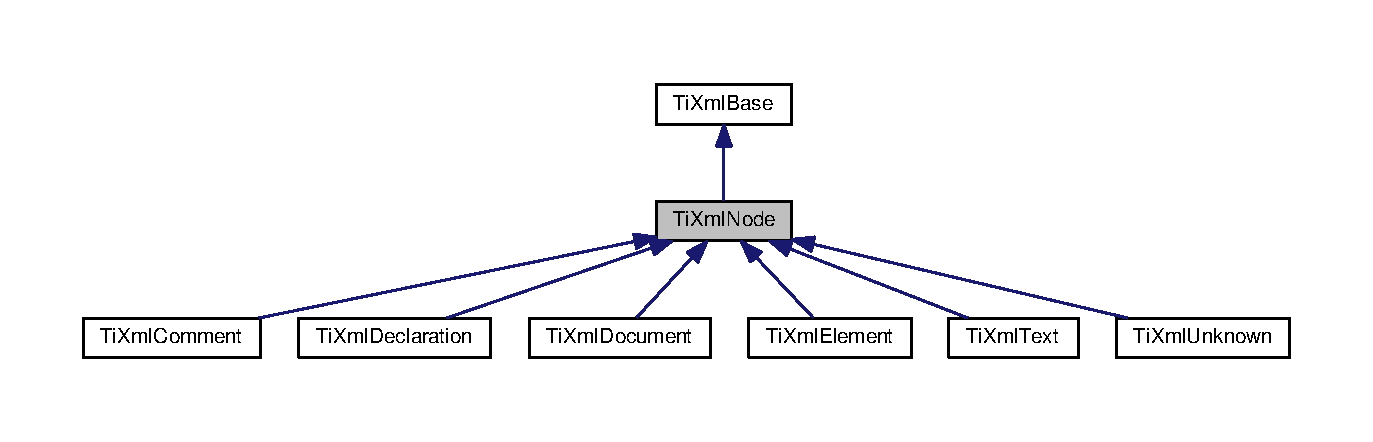
\includegraphics[width=350pt]{classTiXmlNode__inherit__graph}
\end{center}
\end{figure}


Collaboration diagram for Ti\+Xml\+Node\+:\nopagebreak
\begin{figure}[H]
\begin{center}
\leavevmode
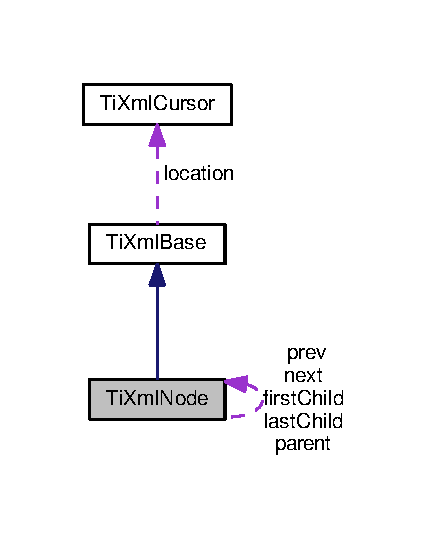
\includegraphics[width=206pt]{classTiXmlNode__coll__graph}
\end{center}
\end{figure}
\subsection*{Public Types}
\begin{DoxyCompactItemize}
\item 
enum \hyperlink{classTiXmlNode_a836eded4920ab9e9ef28496f48cd95a2}{Node\+Type} \{ \\*
{\bfseries T\+I\+N\+Y\+X\+M\+L\+\_\+\+D\+O\+C\+U\+M\+E\+NT}, 
{\bfseries T\+I\+N\+Y\+X\+M\+L\+\_\+\+E\+L\+E\+M\+E\+NT}, 
{\bfseries T\+I\+N\+Y\+X\+M\+L\+\_\+\+C\+O\+M\+M\+E\+NT}, 
{\bfseries T\+I\+N\+Y\+X\+M\+L\+\_\+\+U\+N\+K\+N\+O\+WN}, 
\\*
{\bfseries T\+I\+N\+Y\+X\+M\+L\+\_\+\+T\+E\+XT}, 
{\bfseries T\+I\+N\+Y\+X\+M\+L\+\_\+\+D\+E\+C\+L\+A\+R\+A\+T\+I\+ON}, 
{\bfseries T\+I\+N\+Y\+X\+M\+L\+\_\+\+T\+Y\+P\+E\+C\+O\+U\+NT}
 \}
\end{DoxyCompactItemize}
\subsection*{Public Member Functions}
\begin{DoxyCompactItemize}
\item 
const char $\ast$ \hyperlink{classTiXmlNode_a77943eb90d12c2892b1337a9f5918b41}{Value} () const 
\item 
const T\+I\+X\+M\+L\+\_\+\+S\+T\+R\+I\+NG \& {\bfseries Value\+T\+Str} () const \hypertarget{classTiXmlNode_a83ece13d2ea66dac66e0b21332229239}{}\label{classTiXmlNode_a83ece13d2ea66dac66e0b21332229239}

\item 
void \hyperlink{classTiXmlNode_a2a38329ca5d3f28f98ce932b8299ae90}{Set\+Value} (const char $\ast$\+\_\+value)
\item 
void \hyperlink{classTiXmlNode_a708e7f953df61d4d2d12f73171550a4b}{Clear} ()\hypertarget{classTiXmlNode_a708e7f953df61d4d2d12f73171550a4b}{}\label{classTiXmlNode_a708e7f953df61d4d2d12f73171550a4b}

\begin{DoxyCompactList}\small\item\em Delete all the children of this node. Does not affect \textquotesingle{}this\textquotesingle{}. \end{DoxyCompactList}\item 
\hyperlink{classTiXmlNode}{Ti\+Xml\+Node} $\ast$ \hyperlink{classTiXmlNode_ab643043132ffd794f8602685d34a982e}{Parent} ()\hypertarget{classTiXmlNode_ab643043132ffd794f8602685d34a982e}{}\label{classTiXmlNode_ab643043132ffd794f8602685d34a982e}

\begin{DoxyCompactList}\small\item\em One step up the D\+OM. \end{DoxyCompactList}\item 
const \hyperlink{classTiXmlNode}{Ti\+Xml\+Node} $\ast$ {\bfseries Parent} () const \hypertarget{classTiXmlNode_a78878709e53066f06eb4fcbcdd3a5260}{}\label{classTiXmlNode_a78878709e53066f06eb4fcbcdd3a5260}

\item 
const \hyperlink{classTiXmlNode}{Ti\+Xml\+Node} $\ast$ \hyperlink{classTiXmlNode_a44c8eee26bbe2d1b2762038df9dde2f0}{First\+Child} () const \hypertarget{classTiXmlNode_a44c8eee26bbe2d1b2762038df9dde2f0}{}\label{classTiXmlNode_a44c8eee26bbe2d1b2762038df9dde2f0}

\begin{DoxyCompactList}\small\item\em The first child of this node. Will be null if there are no children. \end{DoxyCompactList}\item 
\hyperlink{classTiXmlNode}{Ti\+Xml\+Node} $\ast$ {\bfseries First\+Child} ()\hypertarget{classTiXmlNode_a5e97d69b7c0ebd27fb7286be56559b77}{}\label{classTiXmlNode_a5e97d69b7c0ebd27fb7286be56559b77}

\item 
const \hyperlink{classTiXmlNode}{Ti\+Xml\+Node} $\ast$ \hyperlink{classTiXmlNode_ab5f722624113c8203227de4f56576d31}{First\+Child} (const char $\ast$value) const 
\item 
\hyperlink{classTiXmlNode}{Ti\+Xml\+Node} $\ast$ \hyperlink{classTiXmlNode_abc8bf32be6419ec453a731868de19554}{First\+Child} (const char $\ast$\+\_\+value)\hypertarget{classTiXmlNode_abc8bf32be6419ec453a731868de19554}{}\label{classTiXmlNode_abc8bf32be6419ec453a731868de19554}

\begin{DoxyCompactList}\small\item\em The first child of this node with the matching \textquotesingle{}value\textquotesingle{}. Will be null if none found. \end{DoxyCompactList}\item 
const \hyperlink{classTiXmlNode}{Ti\+Xml\+Node} $\ast$ {\bfseries Last\+Child} () const \hypertarget{classTiXmlNode_a6d671107e00cca1d28cb2d7f3a87a21e}{}\label{classTiXmlNode_a6d671107e00cca1d28cb2d7f3a87a21e}

\item 
\hyperlink{classTiXmlNode}{Ti\+Xml\+Node} $\ast$ \hyperlink{classTiXmlNode_a6432d2b2495f6caf9cb4278df706a031}{Last\+Child} ()\hypertarget{classTiXmlNode_a6432d2b2495f6caf9cb4278df706a031}{}\label{classTiXmlNode_a6432d2b2495f6caf9cb4278df706a031}

\begin{DoxyCompactList}\small\item\em The last child of this node. Will be null if there are no children. \end{DoxyCompactList}\item 
const \hyperlink{classTiXmlNode}{Ti\+Xml\+Node} $\ast$ {\bfseries Last\+Child} (const char $\ast$value) const \hypertarget{classTiXmlNode_acdd3fdc436aa7433023310a041e5e63f}{}\label{classTiXmlNode_acdd3fdc436aa7433023310a041e5e63f}

\item 
\hyperlink{classTiXmlNode}{Ti\+Xml\+Node} $\ast$ \hyperlink{classTiXmlNode_abad5bf1059c48127b958711ef89e8e5d}{Last\+Child} (const char $\ast$\+\_\+value)\hypertarget{classTiXmlNode_abad5bf1059c48127b958711ef89e8e5d}{}\label{classTiXmlNode_abad5bf1059c48127b958711ef89e8e5d}

\begin{DoxyCompactList}\small\item\em The last child of this node matching \textquotesingle{}value\textquotesingle{}. Will be null if there are no children. \end{DoxyCompactList}\item 
const \hyperlink{classTiXmlNode}{Ti\+Xml\+Node} $\ast$ \hyperlink{classTiXmlNode_aaef7ac3978c4bb1cc8a24ffae7bced75}{Iterate\+Children} (const \hyperlink{classTiXmlNode}{Ti\+Xml\+Node} $\ast$previous) const 
\item 
\hyperlink{classTiXmlNode}{Ti\+Xml\+Node} $\ast$ {\bfseries Iterate\+Children} (const \hyperlink{classTiXmlNode}{Ti\+Xml\+Node} $\ast$previous)\hypertarget{classTiXmlNode_a2358e747118fdbf0e467b1e4f7d03de1}{}\label{classTiXmlNode_a2358e747118fdbf0e467b1e4f7d03de1}

\item 
const \hyperlink{classTiXmlNode}{Ti\+Xml\+Node} $\ast$ \hyperlink{classTiXmlNode_af2b86dbe25d3d26fa48180edc5e2a9fc}{Iterate\+Children} (const char $\ast$value, const \hyperlink{classTiXmlNode}{Ti\+Xml\+Node} $\ast$previous) const \hypertarget{classTiXmlNode_af2b86dbe25d3d26fa48180edc5e2a9fc}{}\label{classTiXmlNode_af2b86dbe25d3d26fa48180edc5e2a9fc}

\begin{DoxyCompactList}\small\item\em This flavor of Iterate\+Children searches for children with a particular \textquotesingle{}value\textquotesingle{}. \end{DoxyCompactList}\item 
\hyperlink{classTiXmlNode}{Ti\+Xml\+Node} $\ast$ {\bfseries Iterate\+Children} (const char $\ast$\+\_\+value, const \hyperlink{classTiXmlNode}{Ti\+Xml\+Node} $\ast$previous)\hypertarget{classTiXmlNode_a67ba8275e533e6f76340236c42ea0aea}{}\label{classTiXmlNode_a67ba8275e533e6f76340236c42ea0aea}

\item 
\hyperlink{classTiXmlNode}{Ti\+Xml\+Node} $\ast$ \hyperlink{classTiXmlNode_af287a913ce46d8dbf7ef24fec69bbaf0}{Insert\+End\+Child} (const \hyperlink{classTiXmlNode}{Ti\+Xml\+Node} \&add\+This)
\item 
\hyperlink{classTiXmlNode}{Ti\+Xml\+Node} $\ast$ \hyperlink{classTiXmlNode_a1a881212554b759865f6cac79a851d38}{Link\+End\+Child} (\hyperlink{classTiXmlNode}{Ti\+Xml\+Node} $\ast$add\+This)
\item 
\hyperlink{classTiXmlNode}{Ti\+Xml\+Node} $\ast$ \hyperlink{classTiXmlNode_a71e54e393336382bc9875f64aab5cb15}{Insert\+Before\+Child} (\hyperlink{classTiXmlNode}{Ti\+Xml\+Node} $\ast$before\+This, const \hyperlink{classTiXmlNode}{Ti\+Xml\+Node} \&add\+This)
\item 
\hyperlink{classTiXmlNode}{Ti\+Xml\+Node} $\ast$ \hyperlink{classTiXmlNode_a274db3292218202805c093f66a964cb5}{Insert\+After\+Child} (\hyperlink{classTiXmlNode}{Ti\+Xml\+Node} $\ast$after\+This, const \hyperlink{classTiXmlNode}{Ti\+Xml\+Node} \&add\+This)
\item 
\hyperlink{classTiXmlNode}{Ti\+Xml\+Node} $\ast$ \hyperlink{classTiXmlNode_a543208c2c801c84a213529541e904b9f}{Replace\+Child} (\hyperlink{classTiXmlNode}{Ti\+Xml\+Node} $\ast$replace\+This, const \hyperlink{classTiXmlNode}{Ti\+Xml\+Node} \&with\+This)
\item 
bool \hyperlink{classTiXmlNode_ae19d8510efc90596552f4feeac9a8fbf}{Remove\+Child} (\hyperlink{classTiXmlNode}{Ti\+Xml\+Node} $\ast$remove\+This)\hypertarget{classTiXmlNode_ae19d8510efc90596552f4feeac9a8fbf}{}\label{classTiXmlNode_ae19d8510efc90596552f4feeac9a8fbf}

\begin{DoxyCompactList}\small\item\em Delete a child of this node. \end{DoxyCompactList}\item 
const \hyperlink{classTiXmlNode}{Ti\+Xml\+Node} $\ast$ \hyperlink{classTiXmlNode_ac2cd892768726270e511b2ab32de4d10}{Previous\+Sibling} () const \hypertarget{classTiXmlNode_ac2cd892768726270e511b2ab32de4d10}{}\label{classTiXmlNode_ac2cd892768726270e511b2ab32de4d10}

\begin{DoxyCompactList}\small\item\em Navigate to a sibling node. \end{DoxyCompactList}\item 
\hyperlink{classTiXmlNode}{Ti\+Xml\+Node} $\ast$ {\bfseries Previous\+Sibling} ()\hypertarget{classTiXmlNode_af8c0642ad6ecc03f62953e68896ed1cc}{}\label{classTiXmlNode_af8c0642ad6ecc03f62953e68896ed1cc}

\item 
const \hyperlink{classTiXmlNode}{Ti\+Xml\+Node} $\ast$ \hyperlink{classTiXmlNode_abbb3b8c1f38fa7b9e52d584a4aeca795}{Previous\+Sibling} (const char $\ast$) const \hypertarget{classTiXmlNode_abbb3b8c1f38fa7b9e52d584a4aeca795}{}\label{classTiXmlNode_abbb3b8c1f38fa7b9e52d584a4aeca795}

\begin{DoxyCompactList}\small\item\em Navigate to a sibling node. \end{DoxyCompactList}\item 
\hyperlink{classTiXmlNode}{Ti\+Xml\+Node} $\ast$ {\bfseries Previous\+Sibling} (const char $\ast$\+\_\+prev)\hypertarget{classTiXmlNode_a6c977049207177ef21b51972315c2053}{}\label{classTiXmlNode_a6c977049207177ef21b51972315c2053}

\item 
const \hyperlink{classTiXmlNode}{Ti\+Xml\+Node} $\ast$ \hyperlink{classTiXmlNode_af854baeba384f5fe9859f5aee03b548e}{Next\+Sibling} () const \hypertarget{classTiXmlNode_af854baeba384f5fe9859f5aee03b548e}{}\label{classTiXmlNode_af854baeba384f5fe9859f5aee03b548e}

\begin{DoxyCompactList}\small\item\em Navigate to a sibling node. \end{DoxyCompactList}\item 
\hyperlink{classTiXmlNode}{Ti\+Xml\+Node} $\ast$ {\bfseries Next\+Sibling} ()\hypertarget{classTiXmlNode_a4d05f7b1d7b470ac6887edd072d4892a}{}\label{classTiXmlNode_a4d05f7b1d7b470ac6887edd072d4892a}

\item 
const \hyperlink{classTiXmlNode}{Ti\+Xml\+Node} $\ast$ \hyperlink{classTiXmlNode_acaf9dc17531ac041f602f9ad579573ea}{Next\+Sibling} (const char $\ast$) const \hypertarget{classTiXmlNode_acaf9dc17531ac041f602f9ad579573ea}{}\label{classTiXmlNode_acaf9dc17531ac041f602f9ad579573ea}

\begin{DoxyCompactList}\small\item\em Navigate to a sibling node with the given \textquotesingle{}value\textquotesingle{}. \end{DoxyCompactList}\item 
\hyperlink{classTiXmlNode}{Ti\+Xml\+Node} $\ast$ {\bfseries Next\+Sibling} (const char $\ast$\+\_\+next)\hypertarget{classTiXmlNode_a4080bc5cc8a5c139e7cf308669e850fc}{}\label{classTiXmlNode_a4080bc5cc8a5c139e7cf308669e850fc}

\item 
const \hyperlink{classTiXmlElement}{Ti\+Xml\+Element} $\ast$ \hyperlink{classTiXmlNode_a7667217e269e0da01d1f82aee94d1a3d}{Next\+Sibling\+Element} () const 
\item 
\hyperlink{classTiXmlElement}{Ti\+Xml\+Element} $\ast$ {\bfseries Next\+Sibling\+Element} ()\hypertarget{classTiXmlNode_a1b211cb5034655a04358e0e2f6fc5010}{}\label{classTiXmlNode_a1b211cb5034655a04358e0e2f6fc5010}

\item 
const \hyperlink{classTiXmlElement}{Ti\+Xml\+Element} $\ast$ \hyperlink{classTiXmlNode_a3d7897999f99cf4870dd59df6331d7ff}{Next\+Sibling\+Element} (const char $\ast$) const 
\item 
\hyperlink{classTiXmlElement}{Ti\+Xml\+Element} $\ast$ {\bfseries Next\+Sibling\+Element} (const char $\ast$\+\_\+next)\hypertarget{classTiXmlNode_a6e1ac6b800e18049bc75e9f8e63a8e5f}{}\label{classTiXmlNode_a6e1ac6b800e18049bc75e9f8e63a8e5f}

\item 
const \hyperlink{classTiXmlElement}{Ti\+Xml\+Element} $\ast$ \hyperlink{classTiXmlNode_ab1f8d8e70d88aea4c5efedfe00862d55}{First\+Child\+Element} () const \hypertarget{classTiXmlNode_ab1f8d8e70d88aea4c5efedfe00862d55}{}\label{classTiXmlNode_ab1f8d8e70d88aea4c5efedfe00862d55}

\begin{DoxyCompactList}\small\item\em Convenience function to get through elements. \end{DoxyCompactList}\item 
\hyperlink{classTiXmlElement}{Ti\+Xml\+Element} $\ast$ {\bfseries First\+Child\+Element} ()\hypertarget{classTiXmlNode_aa0fecff1f3866ab33a8a25506e95db1d}{}\label{classTiXmlNode_aa0fecff1f3866ab33a8a25506e95db1d}

\item 
const \hyperlink{classTiXmlElement}{Ti\+Xml\+Element} $\ast$ \hyperlink{classTiXmlNode_a0ec361bfef1cf1978d060295f597e0d9}{First\+Child\+Element} (const char $\ast$\+\_\+value) const \hypertarget{classTiXmlNode_a0ec361bfef1cf1978d060295f597e0d9}{}\label{classTiXmlNode_a0ec361bfef1cf1978d060295f597e0d9}

\begin{DoxyCompactList}\small\item\em Convenience function to get through elements. \end{DoxyCompactList}\item 
\hyperlink{classTiXmlElement}{Ti\+Xml\+Element} $\ast$ {\bfseries First\+Child\+Element} (const char $\ast$\+\_\+value)\hypertarget{classTiXmlNode_a6936ae323675071808ac4840379e57f5}{}\label{classTiXmlNode_a6936ae323675071808ac4840379e57f5}

\item 
int \hyperlink{classTiXmlNode_a57b99d5c97d67a42b9752f5210a1ba5e}{Type} () const 
\item 
const \hyperlink{classTiXmlDocument}{Ti\+Xml\+Document} $\ast$ \hyperlink{classTiXmlNode_aa66f4ebcd175204a168ed7c2d7b43071}{Get\+Document} () const 
\item 
\hyperlink{classTiXmlDocument}{Ti\+Xml\+Document} $\ast$ {\bfseries Get\+Document} ()\hypertarget{classTiXmlNode_a7b2372c0e7adfb32f5b6902fe49a39b2}{}\label{classTiXmlNode_a7b2372c0e7adfb32f5b6902fe49a39b2}

\item 
bool \hyperlink{classTiXmlNode_aeed21ad30630ef6e7faf096127edc9f3}{No\+Children} () const \hypertarget{classTiXmlNode_aeed21ad30630ef6e7faf096127edc9f3}{}\label{classTiXmlNode_aeed21ad30630ef6e7faf096127edc9f3}

\begin{DoxyCompactList}\small\item\em Returns true if this node has no children. \end{DoxyCompactList}\item 
virtual const \hyperlink{classTiXmlDocument}{Ti\+Xml\+Document} $\ast$ \hyperlink{classTiXmlNode_a8a4cda4b15c29f64cff419309aebed08}{To\+Document} () const \hypertarget{classTiXmlNode_a8a4cda4b15c29f64cff419309aebed08}{}\label{classTiXmlNode_a8a4cda4b15c29f64cff419309aebed08}

\begin{DoxyCompactList}\small\item\em Cast to a more defined type. Will return null if not of the requested type. \end{DoxyCompactList}\item 
virtual const \hyperlink{classTiXmlElement}{Ti\+Xml\+Element} $\ast$ \hyperlink{classTiXmlNode_a72abed96dc9667ab9e0a2a275301bb1c}{To\+Element} () const \hypertarget{classTiXmlNode_a72abed96dc9667ab9e0a2a275301bb1c}{}\label{classTiXmlNode_a72abed96dc9667ab9e0a2a275301bb1c}

\begin{DoxyCompactList}\small\item\em Cast to a more defined type. Will return null if not of the requested type. \end{DoxyCompactList}\item 
virtual const \hyperlink{classTiXmlComment}{Ti\+Xml\+Comment} $\ast$ \hyperlink{classTiXmlNode_aa0a5086f9eaee910bbfdc7f975e26574}{To\+Comment} () const \hypertarget{classTiXmlNode_aa0a5086f9eaee910bbfdc7f975e26574}{}\label{classTiXmlNode_aa0a5086f9eaee910bbfdc7f975e26574}

\begin{DoxyCompactList}\small\item\em Cast to a more defined type. Will return null if not of the requested type. \end{DoxyCompactList}\item 
virtual const \hyperlink{classTiXmlUnknown}{Ti\+Xml\+Unknown} $\ast$ \hyperlink{classTiXmlNode_afd7205cf31d7a376929f8a36930627a2}{To\+Unknown} () const \hypertarget{classTiXmlNode_afd7205cf31d7a376929f8a36930627a2}{}\label{classTiXmlNode_afd7205cf31d7a376929f8a36930627a2}

\begin{DoxyCompactList}\small\item\em Cast to a more defined type. Will return null if not of the requested type. \end{DoxyCompactList}\item 
virtual const \hyperlink{classTiXmlText}{Ti\+Xml\+Text} $\ast$ \hyperlink{classTiXmlNode_a95a46a52c525992d6b4ee08beb14cd69}{To\+Text} () const \hypertarget{classTiXmlNode_a95a46a52c525992d6b4ee08beb14cd69}{}\label{classTiXmlNode_a95a46a52c525992d6b4ee08beb14cd69}

\begin{DoxyCompactList}\small\item\em Cast to a more defined type. Will return null if not of the requested type. \end{DoxyCompactList}\item 
virtual const \hyperlink{classTiXmlDeclaration}{Ti\+Xml\+Declaration} $\ast$ \hyperlink{classTiXmlNode_a9f43e6984fc7d4afd6eb32714c6b7b72}{To\+Declaration} () const \hypertarget{classTiXmlNode_a9f43e6984fc7d4afd6eb32714c6b7b72}{}\label{classTiXmlNode_a9f43e6984fc7d4afd6eb32714c6b7b72}

\begin{DoxyCompactList}\small\item\em Cast to a more defined type. Will return null if not of the requested type. \end{DoxyCompactList}\item 
virtual \hyperlink{classTiXmlDocument}{Ti\+Xml\+Document} $\ast$ \hyperlink{classTiXmlNode_a6a4c8ac28ee7a745d059db6691e03bae}{To\+Document} ()\hypertarget{classTiXmlNode_a6a4c8ac28ee7a745d059db6691e03bae}{}\label{classTiXmlNode_a6a4c8ac28ee7a745d059db6691e03bae}

\begin{DoxyCompactList}\small\item\em Cast to a more defined type. Will return null if not of the requested type. \end{DoxyCompactList}\item 
virtual \hyperlink{classTiXmlElement}{Ti\+Xml\+Element} $\ast$ \hyperlink{classTiXmlNode_aa65d000223187d22a4dcebd7479e9ebc}{To\+Element} ()\hypertarget{classTiXmlNode_aa65d000223187d22a4dcebd7479e9ebc}{}\label{classTiXmlNode_aa65d000223187d22a4dcebd7479e9ebc}

\begin{DoxyCompactList}\small\item\em Cast to a more defined type. Will return null if not of the requested type. \end{DoxyCompactList}\item 
virtual \hyperlink{classTiXmlComment}{Ti\+Xml\+Comment} $\ast$ \hyperlink{classTiXmlNode_a383e06a0787f7063953934867990f849}{To\+Comment} ()\hypertarget{classTiXmlNode_a383e06a0787f7063953934867990f849}{}\label{classTiXmlNode_a383e06a0787f7063953934867990f849}

\begin{DoxyCompactList}\small\item\em Cast to a more defined type. Will return null if not of the requested type. \end{DoxyCompactList}\item 
virtual \hyperlink{classTiXmlUnknown}{Ti\+Xml\+Unknown} $\ast$ \hyperlink{classTiXmlNode_a06de5af852668c7e4af0d09c205f0b0d}{To\+Unknown} ()\hypertarget{classTiXmlNode_a06de5af852668c7e4af0d09c205f0b0d}{}\label{classTiXmlNode_a06de5af852668c7e4af0d09c205f0b0d}

\begin{DoxyCompactList}\small\item\em Cast to a more defined type. Will return null if not of the requested type. \end{DoxyCompactList}\item 
virtual \hyperlink{classTiXmlText}{Ti\+Xml\+Text} $\ast$ \hyperlink{classTiXmlNode_a3ddfbcac78fbea041fad57e5c6d60a03}{To\+Text} ()\hypertarget{classTiXmlNode_a3ddfbcac78fbea041fad57e5c6d60a03}{}\label{classTiXmlNode_a3ddfbcac78fbea041fad57e5c6d60a03}

\begin{DoxyCompactList}\small\item\em Cast to a more defined type. Will return null if not of the requested type. \end{DoxyCompactList}\item 
virtual \hyperlink{classTiXmlDeclaration}{Ti\+Xml\+Declaration} $\ast$ \hyperlink{classTiXmlNode_a4027136ca820ff4a636b607231b6a6df}{To\+Declaration} ()\hypertarget{classTiXmlNode_a4027136ca820ff4a636b607231b6a6df}{}\label{classTiXmlNode_a4027136ca820ff4a636b607231b6a6df}

\begin{DoxyCompactList}\small\item\em Cast to a more defined type. Will return null if not of the requested type. \end{DoxyCompactList}\item 
virtual \hyperlink{classTiXmlNode}{Ti\+Xml\+Node} $\ast$ \hyperlink{classTiXmlNode_a4508cc3a2d7a98e96a54cc09c37a78a4}{Clone} () const =0
\item 
virtual bool \hyperlink{classTiXmlNode_acc0f88b7462c6cb73809d410a4f5bb86}{Accept} (\hyperlink{classTiXmlVisitor}{Ti\+Xml\+Visitor} $\ast$visitor) const =0
\end{DoxyCompactItemize}
\subsection*{Protected Member Functions}
\begin{DoxyCompactItemize}
\item 
{\bfseries Ti\+Xml\+Node} (\hyperlink{classTiXmlNode_a836eded4920ab9e9ef28496f48cd95a2}{Node\+Type} \+\_\+type)\hypertarget{classTiXmlNode_a3f46721695868667113c7487ff123f20}{}\label{classTiXmlNode_a3f46721695868667113c7487ff123f20}

\item 
void {\bfseries Copy\+To} (\hyperlink{classTiXmlNode}{Ti\+Xml\+Node} $\ast$target) const \hypertarget{classTiXmlNode_ab6056978923ad8350fb5164af32d8038}{}\label{classTiXmlNode_ab6056978923ad8350fb5164af32d8038}

\item 
\hyperlink{classTiXmlNode}{Ti\+Xml\+Node} $\ast$ {\bfseries Identify} (const char $\ast$start, Ti\+Xml\+Encoding encoding)\hypertarget{classTiXmlNode_ac1e3a8e7578be463b04617786120c2bb}{}\label{classTiXmlNode_ac1e3a8e7578be463b04617786120c2bb}

\end{DoxyCompactItemize}
\subsection*{Protected Attributes}
\begin{DoxyCompactItemize}
\item 
\hyperlink{classTiXmlNode}{Ti\+Xml\+Node} $\ast$ {\bfseries parent}\hypertarget{classTiXmlNode_a662c4de61244e4fa5bd4e2d8c63143a5}{}\label{classTiXmlNode_a662c4de61244e4fa5bd4e2d8c63143a5}

\item 
\hyperlink{classTiXmlNode_a836eded4920ab9e9ef28496f48cd95a2}{Node\+Type} {\bfseries type}\hypertarget{classTiXmlNode_a2619c6379181c16ba95ae6922e2ca839}{}\label{classTiXmlNode_a2619c6379181c16ba95ae6922e2ca839}

\item 
\hyperlink{classTiXmlNode}{Ti\+Xml\+Node} $\ast$ {\bfseries first\+Child}\hypertarget{classTiXmlNode_af749fb7f22010b80e8f904c32653d50e}{}\label{classTiXmlNode_af749fb7f22010b80e8f904c32653d50e}

\item 
\hyperlink{classTiXmlNode}{Ti\+Xml\+Node} $\ast$ {\bfseries last\+Child}\hypertarget{classTiXmlNode_a5b30756d21b304580d22a841ec9d61f8}{}\label{classTiXmlNode_a5b30756d21b304580d22a841ec9d61f8}

\item 
T\+I\+X\+M\+L\+\_\+\+S\+T\+R\+I\+NG {\bfseries value}\hypertarget{classTiXmlNode_aead528b3cedc33c16a6c539872c7cc8b}{}\label{classTiXmlNode_aead528b3cedc33c16a6c539872c7cc8b}

\item 
\hyperlink{classTiXmlNode}{Ti\+Xml\+Node} $\ast$ {\bfseries prev}\hypertarget{classTiXmlNode_a9c5370ea2cbfd9f0e0f7b30a57fd68f5}{}\label{classTiXmlNode_a9c5370ea2cbfd9f0e0f7b30a57fd68f5}

\item 
\hyperlink{classTiXmlNode}{Ti\+Xml\+Node} $\ast$ {\bfseries next}\hypertarget{classTiXmlNode_a2f329cc993d2d34df76e17dcbb776b45}{}\label{classTiXmlNode_a2f329cc993d2d34df76e17dcbb776b45}

\end{DoxyCompactItemize}
\subsection*{Friends}
\begin{DoxyCompactItemize}
\item 
class {\bfseries Ti\+Xml\+Document}\hypertarget{classTiXmlNode_a173617f6dfe902cf484ce5552b950475}{}\label{classTiXmlNode_a173617f6dfe902cf484ce5552b950475}

\item 
class {\bfseries Ti\+Xml\+Element}\hypertarget{classTiXmlNode_ab6592e32cb9132be517cc12a70564c4b}{}\label{classTiXmlNode_ab6592e32cb9132be517cc12a70564c4b}

\end{DoxyCompactItemize}
\subsection*{Additional Inherited Members}


\subsection{Detailed Description}
The parent class for everything in the Document Object Model. (Except for attributes). Nodes have siblings, a parent, and children. A node can be in a document, or stand on its own. The type of a \hyperlink{classTiXmlNode}{Ti\+Xml\+Node} can be queried, and it can be cast to its more defined type. 

\subsection{Member Enumeration Documentation}
\index{Ti\+Xml\+Node@{Ti\+Xml\+Node}!Node\+Type@{Node\+Type}}
\index{Node\+Type@{Node\+Type}!Ti\+Xml\+Node@{Ti\+Xml\+Node}}
\subsubsection[{\texorpdfstring{Node\+Type}{NodeType}}]{\setlength{\rightskip}{0pt plus 5cm}enum {\bf Ti\+Xml\+Node\+::\+Node\+Type}}\hypertarget{classTiXmlNode_a836eded4920ab9e9ef28496f48cd95a2}{}\label{classTiXmlNode_a836eded4920ab9e9ef28496f48cd95a2}
The types of X\+ML nodes supported by Tiny\+Xml. (All the unsupported types are picked up by U\+N\+K\+N\+O\+WN.) 

\subsection{Member Function Documentation}
\index{Ti\+Xml\+Node@{Ti\+Xml\+Node}!Accept@{Accept}}
\index{Accept@{Accept}!Ti\+Xml\+Node@{Ti\+Xml\+Node}}
\subsubsection[{\texorpdfstring{Accept(\+Ti\+Xml\+Visitor $\ast$visitor) const =0}{Accept(TiXmlVisitor *visitor) const =0}}]{\setlength{\rightskip}{0pt plus 5cm}virtual bool Ti\+Xml\+Node\+::\+Accept (
\begin{DoxyParamCaption}
\item[{{\bf Ti\+Xml\+Visitor} $\ast$}]{visitor}
\end{DoxyParamCaption}
) const\hspace{0.3cm}{\ttfamily [pure virtual]}}\hypertarget{classTiXmlNode_acc0f88b7462c6cb73809d410a4f5bb86}{}\label{classTiXmlNode_acc0f88b7462c6cb73809d410a4f5bb86}
Accept a hierchical visit the nodes in the Tiny\+X\+ML D\+OM. Every node in the X\+ML tree will be conditionally visited and the host will be called back via the \hyperlink{classTiXmlVisitor}{Ti\+Xml\+Visitor} interface.

This is essentially a S\+AX interface for Tiny\+X\+ML. (Note however it doesn\textquotesingle{}t re-\/parse the X\+ML for the callbacks, so the performance of Tiny\+X\+ML is unchanged by using this interface versus any other.)

The interface has been based on ideas from\+:


\begin{DoxyItemize}
\item \href{http://www.saxproject.org/}{\tt http\+://www.\+saxproject.\+org/}
\item \href{http://c2.com/cgi/wiki?HierarchicalVisitorPattern}{\tt http\+://c2.\+com/cgi/wiki?\+Hierarchical\+Visitor\+Pattern}
\end{DoxyItemize}

Which are both good references for \char`\"{}visiting\char`\"{}.

An example of using \hyperlink{classTiXmlNode_acc0f88b7462c6cb73809d410a4f5bb86}{Accept()}\+: \begin{DoxyVerb}TiXmlPrinter printer;
tinyxmlDoc.Accept( &printer );
const char* xmlcstr = printer.CStr();
\end{DoxyVerb}
 

Implemented in \hyperlink{classTiXmlDocument_a3daab2f472418ef66315750202f762ae}{Ti\+Xml\+Document}, \hyperlink{classTiXmlUnknown_a4e54d7482e05a837cf83c925cc683380}{Ti\+Xml\+Unknown}, \hyperlink{classTiXmlDeclaration_ab6a6b178161ba9abc2c35058de689864}{Ti\+Xml\+Declaration}, \hyperlink{classTiXmlText_a43b9954ebf679557fac1a4453f337b7c}{Ti\+Xml\+Text}, \hyperlink{classTiXmlComment_a4382de0e50da973f11a23ea5852568bd}{Ti\+Xml\+Comment}, and \hyperlink{classTiXmlElement_a31ab28cc3b892a69254391d6bbe08df3}{Ti\+Xml\+Element}.

\index{Ti\+Xml\+Node@{Ti\+Xml\+Node}!Clone@{Clone}}
\index{Clone@{Clone}!Ti\+Xml\+Node@{Ti\+Xml\+Node}}
\subsubsection[{\texorpdfstring{Clone() const =0}{Clone() const =0}}]{\setlength{\rightskip}{0pt plus 5cm}virtual {\bf Ti\+Xml\+Node}$\ast$ Ti\+Xml\+Node\+::\+Clone (
\begin{DoxyParamCaption}
{}
\end{DoxyParamCaption}
) const\hspace{0.3cm}{\ttfamily [pure virtual]}}\hypertarget{classTiXmlNode_a4508cc3a2d7a98e96a54cc09c37a78a4}{}\label{classTiXmlNode_a4508cc3a2d7a98e96a54cc09c37a78a4}
Create an exact duplicate of this node and return it. The memory must be deleted by the caller. 

Implemented in \hyperlink{classTiXmlDocument_ac9e8f09b23454d953b32d1b65cd1409e}{Ti\+Xml\+Document}, \hyperlink{classTiXmlUnknown_a675c4b2684af35e4c7649b7fd5ae598d}{Ti\+Xml\+Unknown}, \hyperlink{classTiXmlDeclaration_aff8231266d735943d8a7514a9c9822b9}{Ti\+Xml\+Declaration}, \hyperlink{classTiXmlText_adde1869dfb029be50713fbfd8ce4d21f}{Ti\+Xml\+Text}, \hyperlink{classTiXmlComment_a4f6590c9c9a2b63a48972655b78eb853}{Ti\+Xml\+Comment}, and \hyperlink{classTiXmlElement_a13f6df105ebb1e8dc636e75cc883be32}{Ti\+Xml\+Element}.

\index{Ti\+Xml\+Node@{Ti\+Xml\+Node}!First\+Child@{First\+Child}}
\index{First\+Child@{First\+Child}!Ti\+Xml\+Node@{Ti\+Xml\+Node}}
\subsubsection[{\texorpdfstring{First\+Child(const char $\ast$value) const }{FirstChild(const char *value) const }}]{\setlength{\rightskip}{0pt plus 5cm}const {\bf Ti\+Xml\+Node} $\ast$ Ti\+Xml\+Node\+::\+First\+Child (
\begin{DoxyParamCaption}
\item[{const char $\ast$}]{value}
\end{DoxyParamCaption}
) const}\hypertarget{classTiXmlNode_ab5f722624113c8203227de4f56576d31}{}\label{classTiXmlNode_ab5f722624113c8203227de4f56576d31}
The first child of this node with the matching \textquotesingle{}value\textquotesingle{}. Will be null if none found. \index{Ti\+Xml\+Node@{Ti\+Xml\+Node}!Get\+Document@{Get\+Document}}
\index{Get\+Document@{Get\+Document}!Ti\+Xml\+Node@{Ti\+Xml\+Node}}
\subsubsection[{\texorpdfstring{Get\+Document() const }{GetDocument() const }}]{\setlength{\rightskip}{0pt plus 5cm}const {\bf Ti\+Xml\+Document} $\ast$ Ti\+Xml\+Node\+::\+Get\+Document (
\begin{DoxyParamCaption}
{}
\end{DoxyParamCaption}
) const}\hypertarget{classTiXmlNode_aa66f4ebcd175204a168ed7c2d7b43071}{}\label{classTiXmlNode_aa66f4ebcd175204a168ed7c2d7b43071}
Return a pointer to the Document this node lives in. Returns null if not in a document. \index{Ti\+Xml\+Node@{Ti\+Xml\+Node}!Insert\+After\+Child@{Insert\+After\+Child}}
\index{Insert\+After\+Child@{Insert\+After\+Child}!Ti\+Xml\+Node@{Ti\+Xml\+Node}}
\subsubsection[{\texorpdfstring{Insert\+After\+Child(\+Ti\+Xml\+Node $\ast$after\+This, const Ti\+Xml\+Node \&add\+This)}{InsertAfterChild(TiXmlNode *afterThis, const TiXmlNode &addThis)}}]{\setlength{\rightskip}{0pt plus 5cm}{\bf Ti\+Xml\+Node} $\ast$ Ti\+Xml\+Node\+::\+Insert\+After\+Child (
\begin{DoxyParamCaption}
\item[{{\bf Ti\+Xml\+Node} $\ast$}]{after\+This, }
\item[{const {\bf Ti\+Xml\+Node} \&}]{add\+This}
\end{DoxyParamCaption}
)}\hypertarget{classTiXmlNode_a274db3292218202805c093f66a964cb5}{}\label{classTiXmlNode_a274db3292218202805c093f66a964cb5}
Add a new node related to this. Adds a child after the specified child. Returns a pointer to the new object or N\+U\+LL if an error occured. \index{Ti\+Xml\+Node@{Ti\+Xml\+Node}!Insert\+Before\+Child@{Insert\+Before\+Child}}
\index{Insert\+Before\+Child@{Insert\+Before\+Child}!Ti\+Xml\+Node@{Ti\+Xml\+Node}}
\subsubsection[{\texorpdfstring{Insert\+Before\+Child(\+Ti\+Xml\+Node $\ast$before\+This, const Ti\+Xml\+Node \&add\+This)}{InsertBeforeChild(TiXmlNode *beforeThis, const TiXmlNode &addThis)}}]{\setlength{\rightskip}{0pt plus 5cm}{\bf Ti\+Xml\+Node} $\ast$ Ti\+Xml\+Node\+::\+Insert\+Before\+Child (
\begin{DoxyParamCaption}
\item[{{\bf Ti\+Xml\+Node} $\ast$}]{before\+This, }
\item[{const {\bf Ti\+Xml\+Node} \&}]{add\+This}
\end{DoxyParamCaption}
)}\hypertarget{classTiXmlNode_a71e54e393336382bc9875f64aab5cb15}{}\label{classTiXmlNode_a71e54e393336382bc9875f64aab5cb15}
Add a new node related to this. Adds a child before the specified child. Returns a pointer to the new object or N\+U\+LL if an error occured. \index{Ti\+Xml\+Node@{Ti\+Xml\+Node}!Insert\+End\+Child@{Insert\+End\+Child}}
\index{Insert\+End\+Child@{Insert\+End\+Child}!Ti\+Xml\+Node@{Ti\+Xml\+Node}}
\subsubsection[{\texorpdfstring{Insert\+End\+Child(const Ti\+Xml\+Node \&add\+This)}{InsertEndChild(const TiXmlNode &addThis)}}]{\setlength{\rightskip}{0pt plus 5cm}{\bf Ti\+Xml\+Node} $\ast$ Ti\+Xml\+Node\+::\+Insert\+End\+Child (
\begin{DoxyParamCaption}
\item[{const {\bf Ti\+Xml\+Node} \&}]{add\+This}
\end{DoxyParamCaption}
)}\hypertarget{classTiXmlNode_af287a913ce46d8dbf7ef24fec69bbaf0}{}\label{classTiXmlNode_af287a913ce46d8dbf7ef24fec69bbaf0}
Add a new node related to this. Adds a child past the Last\+Child. Returns a pointer to the new object or N\+U\+LL if an error occured. \index{Ti\+Xml\+Node@{Ti\+Xml\+Node}!Iterate\+Children@{Iterate\+Children}}
\index{Iterate\+Children@{Iterate\+Children}!Ti\+Xml\+Node@{Ti\+Xml\+Node}}
\subsubsection[{\texorpdfstring{Iterate\+Children(const Ti\+Xml\+Node $\ast$previous) const }{IterateChildren(const TiXmlNode *previous) const }}]{\setlength{\rightskip}{0pt plus 5cm}const {\bf Ti\+Xml\+Node} $\ast$ Ti\+Xml\+Node\+::\+Iterate\+Children (
\begin{DoxyParamCaption}
\item[{const {\bf Ti\+Xml\+Node} $\ast$}]{previous}
\end{DoxyParamCaption}
) const}\hypertarget{classTiXmlNode_aaef7ac3978c4bb1cc8a24ffae7bced75}{}\label{classTiXmlNode_aaef7ac3978c4bb1cc8a24ffae7bced75}
An alternate way to walk the children of a node. One way to iterate over nodes is\+: \begin{DoxyVerb}    for( child = parent->FirstChild(); child; child = child->NextSibling() )
\end{DoxyVerb}


Iterate\+Children does the same thing with the syntax\+: \begin{DoxyVerb}    child = 0;
    while( child = parent->IterateChildren( child ) )
\end{DoxyVerb}


Iterate\+Children takes the previous child as input and finds the next one. If the previous child is null, it returns the first. Iterate\+Children will return null when done. \index{Ti\+Xml\+Node@{Ti\+Xml\+Node}!Link\+End\+Child@{Link\+End\+Child}}
\index{Link\+End\+Child@{Link\+End\+Child}!Ti\+Xml\+Node@{Ti\+Xml\+Node}}
\subsubsection[{\texorpdfstring{Link\+End\+Child(\+Ti\+Xml\+Node $\ast$add\+This)}{LinkEndChild(TiXmlNode *addThis)}}]{\setlength{\rightskip}{0pt plus 5cm}{\bf Ti\+Xml\+Node} $\ast$ Ti\+Xml\+Node\+::\+Link\+End\+Child (
\begin{DoxyParamCaption}
\item[{{\bf Ti\+Xml\+Node} $\ast$}]{add\+This}
\end{DoxyParamCaption}
)}\hypertarget{classTiXmlNode_a1a881212554b759865f6cac79a851d38}{}\label{classTiXmlNode_a1a881212554b759865f6cac79a851d38}
Add a new node related to this. Adds a child past the Last\+Child.

N\+O\+TE\+: the node to be added is passed by pointer, and will be henceforth owned (and deleted) by tiny\+Xml. This method is efficient and avoids an extra copy, but should be used with care as it uses a different memory model than the other insert functions.

\begin{DoxySeeAlso}{See also}
\hyperlink{classTiXmlNode_af287a913ce46d8dbf7ef24fec69bbaf0}{Insert\+End\+Child} 
\end{DoxySeeAlso}
\index{Ti\+Xml\+Node@{Ti\+Xml\+Node}!Next\+Sibling\+Element@{Next\+Sibling\+Element}}
\index{Next\+Sibling\+Element@{Next\+Sibling\+Element}!Ti\+Xml\+Node@{Ti\+Xml\+Node}}
\subsubsection[{\texorpdfstring{Next\+Sibling\+Element() const }{NextSiblingElement() const }}]{\setlength{\rightskip}{0pt plus 5cm}const {\bf Ti\+Xml\+Element} $\ast$ Ti\+Xml\+Node\+::\+Next\+Sibling\+Element (
\begin{DoxyParamCaption}
{}
\end{DoxyParamCaption}
) const}\hypertarget{classTiXmlNode_a7667217e269e0da01d1f82aee94d1a3d}{}\label{classTiXmlNode_a7667217e269e0da01d1f82aee94d1a3d}
Convenience function to get through elements. Calls Next\+Sibling and To\+Element. Will skip all non-\/\+Element nodes. Returns 0 if there is not another element. \index{Ti\+Xml\+Node@{Ti\+Xml\+Node}!Next\+Sibling\+Element@{Next\+Sibling\+Element}}
\index{Next\+Sibling\+Element@{Next\+Sibling\+Element}!Ti\+Xml\+Node@{Ti\+Xml\+Node}}
\subsubsection[{\texorpdfstring{Next\+Sibling\+Element(const char $\ast$) const }{NextSiblingElement(const char *) const }}]{\setlength{\rightskip}{0pt plus 5cm}const {\bf Ti\+Xml\+Element} $\ast$ Ti\+Xml\+Node\+::\+Next\+Sibling\+Element (
\begin{DoxyParamCaption}
\item[{const char $\ast$}]{\+\_\+value}
\end{DoxyParamCaption}
) const}\hypertarget{classTiXmlNode_a3d7897999f99cf4870dd59df6331d7ff}{}\label{classTiXmlNode_a3d7897999f99cf4870dd59df6331d7ff}
Convenience function to get through elements. Calls Next\+Sibling and To\+Element. Will skip all non-\/\+Element nodes. Returns 0 if there is not another element. \index{Ti\+Xml\+Node@{Ti\+Xml\+Node}!Replace\+Child@{Replace\+Child}}
\index{Replace\+Child@{Replace\+Child}!Ti\+Xml\+Node@{Ti\+Xml\+Node}}
\subsubsection[{\texorpdfstring{Replace\+Child(\+Ti\+Xml\+Node $\ast$replace\+This, const Ti\+Xml\+Node \&with\+This)}{ReplaceChild(TiXmlNode *replaceThis, const TiXmlNode &withThis)}}]{\setlength{\rightskip}{0pt plus 5cm}{\bf Ti\+Xml\+Node} $\ast$ Ti\+Xml\+Node\+::\+Replace\+Child (
\begin{DoxyParamCaption}
\item[{{\bf Ti\+Xml\+Node} $\ast$}]{replace\+This, }
\item[{const {\bf Ti\+Xml\+Node} \&}]{with\+This}
\end{DoxyParamCaption}
)}\hypertarget{classTiXmlNode_a543208c2c801c84a213529541e904b9f}{}\label{classTiXmlNode_a543208c2c801c84a213529541e904b9f}
Replace a child of this node. Returns a pointer to the new object or N\+U\+LL if an error occured. \index{Ti\+Xml\+Node@{Ti\+Xml\+Node}!Set\+Value@{Set\+Value}}
\index{Set\+Value@{Set\+Value}!Ti\+Xml\+Node@{Ti\+Xml\+Node}}
\subsubsection[{\texorpdfstring{Set\+Value(const char $\ast$\+\_\+value)}{SetValue(const char *_value)}}]{\setlength{\rightskip}{0pt plus 5cm}void Ti\+Xml\+Node\+::\+Set\+Value (
\begin{DoxyParamCaption}
\item[{const char $\ast$}]{\+\_\+value}
\end{DoxyParamCaption}
)\hspace{0.3cm}{\ttfamily [inline]}}\hypertarget{classTiXmlNode_a2a38329ca5d3f28f98ce932b8299ae90}{}\label{classTiXmlNode_a2a38329ca5d3f28f98ce932b8299ae90}
Changes the value of the node. Defined as\+: \begin{DoxyVerb}Document:   filename of the xml file
Element:    name of the element
Comment:    the comment text
Unknown:    the tag contents
Text:       the text string
\end{DoxyVerb}
 \index{Ti\+Xml\+Node@{Ti\+Xml\+Node}!Type@{Type}}
\index{Type@{Type}!Ti\+Xml\+Node@{Ti\+Xml\+Node}}
\subsubsection[{\texorpdfstring{Type() const }{Type() const }}]{\setlength{\rightskip}{0pt plus 5cm}int Ti\+Xml\+Node\+::\+Type (
\begin{DoxyParamCaption}
{}
\end{DoxyParamCaption}
) const\hspace{0.3cm}{\ttfamily [inline]}}\hypertarget{classTiXmlNode_a57b99d5c97d67a42b9752f5210a1ba5e}{}\label{classTiXmlNode_a57b99d5c97d67a42b9752f5210a1ba5e}
Query the type (as an enumerated value, above) of this node. The possible types are\+: T\+I\+N\+Y\+X\+M\+L\+\_\+\+D\+O\+C\+U\+M\+E\+NT, T\+I\+N\+Y\+X\+M\+L\+\_\+\+E\+L\+E\+M\+E\+NT, T\+I\+N\+Y\+X\+M\+L\+\_\+\+C\+O\+M\+M\+E\+NT, T\+I\+N\+Y\+X\+M\+L\+\_\+\+U\+N\+K\+N\+O\+WN, T\+I\+N\+Y\+X\+M\+L\+\_\+\+T\+E\+XT, and T\+I\+N\+Y\+X\+M\+L\+\_\+\+D\+E\+C\+L\+A\+R\+A\+T\+I\+ON. \index{Ti\+Xml\+Node@{Ti\+Xml\+Node}!Value@{Value}}
\index{Value@{Value}!Ti\+Xml\+Node@{Ti\+Xml\+Node}}
\subsubsection[{\texorpdfstring{Value() const }{Value() const }}]{\setlength{\rightskip}{0pt plus 5cm}const char$\ast$ Ti\+Xml\+Node\+::\+Value (
\begin{DoxyParamCaption}
{}
\end{DoxyParamCaption}
) const\hspace{0.3cm}{\ttfamily [inline]}}\hypertarget{classTiXmlNode_a77943eb90d12c2892b1337a9f5918b41}{}\label{classTiXmlNode_a77943eb90d12c2892b1337a9f5918b41}
The meaning of \textquotesingle{}value\textquotesingle{} changes for the specific type of \hyperlink{classTiXmlNode}{Ti\+Xml\+Node}. \begin{DoxyVerb}Document:   filename of the xml file
Element:    name of the element
Comment:    the comment text
Unknown:    the tag contents
Text:       the text string
\end{DoxyVerb}


The subclasses will wrap this function. 

The documentation for this class was generated from the following files\+:\begin{DoxyCompactItemize}
\item 
src/tinyxml.\+h\item 
src/tinyxml.\+cpp\item 
src/tinyxmlparser.\+cpp\end{DoxyCompactItemize}

\hypertarget{classTiXmlOutStream}{}\section{Ti\+Xml\+Out\+Stream Class Reference}
\label{classTiXmlOutStream}\index{Ti\+Xml\+Out\+Stream@{Ti\+Xml\+Out\+Stream}}


Inheritance diagram for Ti\+Xml\+Out\+Stream\+:\nopagebreak
\begin{figure}[H]
\begin{center}
\leavevmode
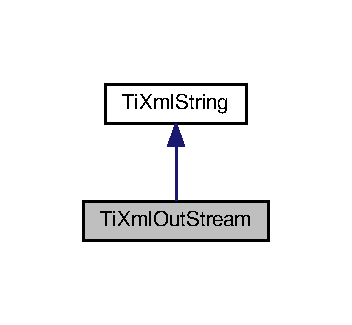
\includegraphics[width=169pt]{classTiXmlOutStream__inherit__graph}
\end{center}
\end{figure}


Collaboration diagram for Ti\+Xml\+Out\+Stream\+:\nopagebreak
\begin{figure}[H]
\begin{center}
\leavevmode
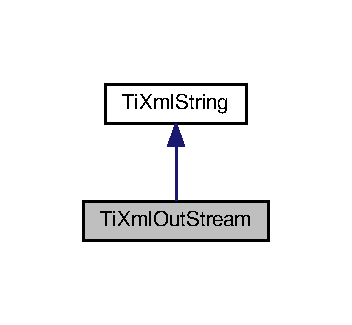
\includegraphics[width=169pt]{classTiXmlOutStream__coll__graph}
\end{center}
\end{figure}
\subsection*{Public Member Functions}
\begin{DoxyCompactItemize}
\item 
\hyperlink{classTiXmlOutStream}{Ti\+Xml\+Out\+Stream} \& {\bfseries operator$<$$<$} (const \hyperlink{classTiXmlString}{Ti\+Xml\+String} \&in)\hypertarget{classTiXmlOutStream_a3640dcb1c0903be3bc6966cdc9a79db6}{}\label{classTiXmlOutStream_a3640dcb1c0903be3bc6966cdc9a79db6}

\item 
\hyperlink{classTiXmlOutStream}{Ti\+Xml\+Out\+Stream} \& {\bfseries operator$<$$<$} (const char $\ast$in)\hypertarget{classTiXmlOutStream_af2117e5a8cbfcb69544804ad2859bfb6}{}\label{classTiXmlOutStream_af2117e5a8cbfcb69544804ad2859bfb6}

\end{DoxyCompactItemize}
\subsection*{Additional Inherited Members}


The documentation for this class was generated from the following file\+:\begin{DoxyCompactItemize}
\item 
src/tinyxml/tinystr.\+h\end{DoxyCompactItemize}

\hypertarget{classTiXmlParsingData}{}\section{Ti\+Xml\+Parsing\+Data Class Reference}
\label{classTiXmlParsingData}\index{Ti\+Xml\+Parsing\+Data@{Ti\+Xml\+Parsing\+Data}}
\subsection*{Public Member Functions}
\begin{DoxyCompactItemize}
\item 
void {\bfseries Stamp} (const char $\ast$now, Ti\+Xml\+Encoding encoding)\hypertarget{classTiXmlParsingData_a65cee8ab77a36c605db08c84b4c30a7d}{}\label{classTiXmlParsingData_a65cee8ab77a36c605db08c84b4c30a7d}

\item 
const \hyperlink{structTiXmlCursor}{Ti\+Xml\+Cursor} \& {\bfseries Cursor} () const \hypertarget{classTiXmlParsingData_a9e63d965fdb53ff4ac711e105269e918}{}\label{classTiXmlParsingData_a9e63d965fdb53ff4ac711e105269e918}

\end{DoxyCompactItemize}
\subsection*{Friends}
\begin{DoxyCompactItemize}
\item 
class {\bfseries Ti\+Xml\+Document}\hypertarget{classTiXmlParsingData_a173617f6dfe902cf484ce5552b950475}{}\label{classTiXmlParsingData_a173617f6dfe902cf484ce5552b950475}

\end{DoxyCompactItemize}


The documentation for this class was generated from the following file\+:\begin{DoxyCompactItemize}
\item 
src/tinyxml/tinyxmlparser.\+cpp\end{DoxyCompactItemize}

\hypertarget{classTiXmlPrinter}{}\section{Ti\+Xml\+Printer Class Reference}
\label{classTiXmlPrinter}\index{Ti\+Xml\+Printer@{Ti\+Xml\+Printer}}


{\ttfamily \#include $<$tinyxml.\+h$>$}



Inheritance diagram for Ti\+Xml\+Printer\+:\nopagebreak
\begin{figure}[H]
\begin{center}
\leavevmode
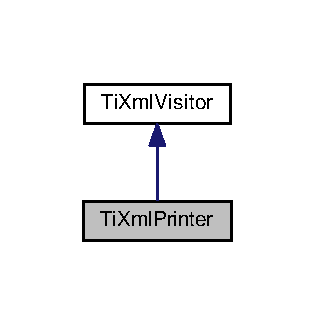
\includegraphics[width=151pt]{classTiXmlPrinter__inherit__graph}
\end{center}
\end{figure}


Collaboration diagram for Ti\+Xml\+Printer\+:\nopagebreak
\begin{figure}[H]
\begin{center}
\leavevmode
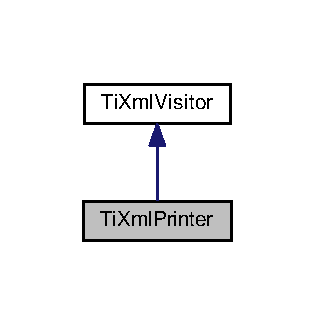
\includegraphics[width=151pt]{classTiXmlPrinter__coll__graph}
\end{center}
\end{figure}
\subsection*{Public Member Functions}
\begin{DoxyCompactItemize}
\item 
virtual bool \hyperlink{classTiXmlPrinter_a2ec73087db26ff4d2c4316c56f861db7}{Visit\+Enter} (const \hyperlink{classTiXmlDocument}{Ti\+Xml\+Document} \&doc)\hypertarget{classTiXmlPrinter_a2ec73087db26ff4d2c4316c56f861db7}{}\label{classTiXmlPrinter_a2ec73087db26ff4d2c4316c56f861db7}

\begin{DoxyCompactList}\small\item\em Visit a document. \end{DoxyCompactList}\item 
virtual bool \hyperlink{classTiXmlPrinter_a0a636046fa589b6d7f3e5bd025b3f33e}{Visit\+Exit} (const \hyperlink{classTiXmlDocument}{Ti\+Xml\+Document} \&doc)\hypertarget{classTiXmlPrinter_a0a636046fa589b6d7f3e5bd025b3f33e}{}\label{classTiXmlPrinter_a0a636046fa589b6d7f3e5bd025b3f33e}

\begin{DoxyCompactList}\small\item\em Visit a document. \end{DoxyCompactList}\item 
virtual bool \hyperlink{classTiXmlPrinter_a6dccaf5ee4979f13877690afe28721e8}{Visit\+Enter} (const \hyperlink{classTiXmlElement}{Ti\+Xml\+Element} \&element, const \hyperlink{classTiXmlAttribute}{Ti\+Xml\+Attribute} $\ast$first\+Attribute)\hypertarget{classTiXmlPrinter_a6dccaf5ee4979f13877690afe28721e8}{}\label{classTiXmlPrinter_a6dccaf5ee4979f13877690afe28721e8}

\begin{DoxyCompactList}\small\item\em Visit an element. \end{DoxyCompactList}\item 
virtual bool \hyperlink{classTiXmlPrinter_ae6a1df8271df4bf62d7873c38e34aa69}{Visit\+Exit} (const \hyperlink{classTiXmlElement}{Ti\+Xml\+Element} \&element)\hypertarget{classTiXmlPrinter_ae6a1df8271df4bf62d7873c38e34aa69}{}\label{classTiXmlPrinter_ae6a1df8271df4bf62d7873c38e34aa69}

\begin{DoxyCompactList}\small\item\em Visit an element. \end{DoxyCompactList}\item 
virtual bool \hyperlink{classTiXmlPrinter_adaf7eec4dc43ad071ff52b60361574f5}{Visit} (const \hyperlink{classTiXmlDeclaration}{Ti\+Xml\+Declaration} \&declaration)\hypertarget{classTiXmlPrinter_adaf7eec4dc43ad071ff52b60361574f5}{}\label{classTiXmlPrinter_adaf7eec4dc43ad071ff52b60361574f5}

\begin{DoxyCompactList}\small\item\em Visit a declaration. \end{DoxyCompactList}\item 
virtual bool \hyperlink{classTiXmlPrinter_a0857c5d32c59b9a257f9a49cb9411df5}{Visit} (const \hyperlink{classTiXmlText}{Ti\+Xml\+Text} \&text)\hypertarget{classTiXmlPrinter_a0857c5d32c59b9a257f9a49cb9411df5}{}\label{classTiXmlPrinter_a0857c5d32c59b9a257f9a49cb9411df5}

\begin{DoxyCompactList}\small\item\em Visit a text node. \end{DoxyCompactList}\item 
virtual bool \hyperlink{classTiXmlPrinter_a9870423f5603630e6142f6bdb66dfb57}{Visit} (const \hyperlink{classTiXmlComment}{Ti\+Xml\+Comment} \&comment)\hypertarget{classTiXmlPrinter_a9870423f5603630e6142f6bdb66dfb57}{}\label{classTiXmlPrinter_a9870423f5603630e6142f6bdb66dfb57}

\begin{DoxyCompactList}\small\item\em Visit a comment node. \end{DoxyCompactList}\item 
virtual bool \hyperlink{classTiXmlPrinter_a08591a15c9a07afa83c24e08b03d6358}{Visit} (const \hyperlink{classTiXmlUnknown}{Ti\+Xml\+Unknown} \&unknown)\hypertarget{classTiXmlPrinter_a08591a15c9a07afa83c24e08b03d6358}{}\label{classTiXmlPrinter_a08591a15c9a07afa83c24e08b03d6358}

\begin{DoxyCompactList}\small\item\em Visit an unknown node. \end{DoxyCompactList}\item 
void \hyperlink{classTiXmlPrinter_a213377a4070c7e625bae59716b089e5e}{Set\+Indent} (const char $\ast$\+\_\+indent)
\item 
const char $\ast$ \hyperlink{classTiXmlPrinter_abb33ec7d4bad6aaeb57f4304394b133d}{Indent} ()\hypertarget{classTiXmlPrinter_abb33ec7d4bad6aaeb57f4304394b133d}{}\label{classTiXmlPrinter_abb33ec7d4bad6aaeb57f4304394b133d}

\begin{DoxyCompactList}\small\item\em Query the indention string. \end{DoxyCompactList}\item 
void \hyperlink{classTiXmlPrinter_a4be1e37e69e3858c59635aa947174fe6}{Set\+Line\+Break} (const char $\ast$\+\_\+line\+Break)
\item 
const char $\ast$ \hyperlink{classTiXmlPrinter_a11f1b4804a460b175ec244eb5724d96d}{Line\+Break} ()\hypertarget{classTiXmlPrinter_a11f1b4804a460b175ec244eb5724d96d}{}\label{classTiXmlPrinter_a11f1b4804a460b175ec244eb5724d96d}

\begin{DoxyCompactList}\small\item\em Query the current line breaking string. \end{DoxyCompactList}\item 
void \hyperlink{classTiXmlPrinter_ab23a90629e374cb1cadca090468bbd19}{Set\+Stream\+Printing} ()
\item 
const char $\ast$ \hyperlink{classTiXmlPrinter_a859eede9597d3e0355b77757be48735e}{C\+Str} ()\hypertarget{classTiXmlPrinter_a859eede9597d3e0355b77757be48735e}{}\label{classTiXmlPrinter_a859eede9597d3e0355b77757be48735e}

\begin{DoxyCompactList}\small\item\em Return the result. \end{DoxyCompactList}\item 
size\+\_\+t \hyperlink{classTiXmlPrinter_ad01375ae9199bd2f48252eaddce3039d}{Size} ()\hypertarget{classTiXmlPrinter_ad01375ae9199bd2f48252eaddce3039d}{}\label{classTiXmlPrinter_ad01375ae9199bd2f48252eaddce3039d}

\begin{DoxyCompactList}\small\item\em Return the length of the result string. \end{DoxyCompactList}\end{DoxyCompactItemize}


\subsection{Detailed Description}
Print to memory functionality. The \hyperlink{classTiXmlPrinter}{Ti\+Xml\+Printer} is useful when you need to\+:


\begin{DoxyEnumerate}
\item Print to memory (especially in non-\/\+S\+TL mode)
\item Control formatting (line endings, etc.)
\end{DoxyEnumerate}

When constructed, the \hyperlink{classTiXmlPrinter}{Ti\+Xml\+Printer} is in its default \char`\"{}pretty printing\char`\"{} mode. Before calling Accept() you can call methods to control the printing of the X\+ML document. After \hyperlink{classTiXmlNode_acc0f88b7462c6cb73809d410a4f5bb86}{Ti\+Xml\+Node\+::\+Accept()} is called, the printed document can be accessed via the \hyperlink{classTiXmlPrinter_a859eede9597d3e0355b77757be48735e}{C\+Str()}, Str(), and \hyperlink{classTiXmlPrinter_ad01375ae9199bd2f48252eaddce3039d}{Size()} methods.

\hyperlink{classTiXmlPrinter}{Ti\+Xml\+Printer} uses the Visitor A\+PI. \begin{DoxyVerb}TiXmlPrinter printer;
printer.SetIndent( "\t" );

doc.Accept( &printer );
fprintf( stdout, "%s", printer.CStr() );
\end{DoxyVerb}
 

\subsection{Member Function Documentation}
\index{Ti\+Xml\+Printer@{Ti\+Xml\+Printer}!Set\+Indent@{Set\+Indent}}
\index{Set\+Indent@{Set\+Indent}!Ti\+Xml\+Printer@{Ti\+Xml\+Printer}}
\subsubsection[{\texorpdfstring{Set\+Indent(const char $\ast$\+\_\+indent)}{SetIndent(const char *_indent)}}]{\setlength{\rightskip}{0pt plus 5cm}void Ti\+Xml\+Printer\+::\+Set\+Indent (
\begin{DoxyParamCaption}
\item[{const char $\ast$}]{\+\_\+indent}
\end{DoxyParamCaption}
)\hspace{0.3cm}{\ttfamily [inline]}}\hypertarget{classTiXmlPrinter_a213377a4070c7e625bae59716b089e5e}{}\label{classTiXmlPrinter_a213377a4070c7e625bae59716b089e5e}
Set the indent characters for printing. By default 4 spaces but tab () is also useful, or null/empty string for no indentation. \index{Ti\+Xml\+Printer@{Ti\+Xml\+Printer}!Set\+Line\+Break@{Set\+Line\+Break}}
\index{Set\+Line\+Break@{Set\+Line\+Break}!Ti\+Xml\+Printer@{Ti\+Xml\+Printer}}
\subsubsection[{\texorpdfstring{Set\+Line\+Break(const char $\ast$\+\_\+line\+Break)}{SetLineBreak(const char *_lineBreak)}}]{\setlength{\rightskip}{0pt plus 5cm}void Ti\+Xml\+Printer\+::\+Set\+Line\+Break (
\begin{DoxyParamCaption}
\item[{const char $\ast$}]{\+\_\+line\+Break}
\end{DoxyParamCaption}
)\hspace{0.3cm}{\ttfamily [inline]}}\hypertarget{classTiXmlPrinter_a4be1e37e69e3858c59635aa947174fe6}{}\label{classTiXmlPrinter_a4be1e37e69e3858c59635aa947174fe6}
Set the line breaking string. By default set to newline (~\newline
). Some operating systems prefer other characters, or can be set to the null/empty string for no indenation. \index{Ti\+Xml\+Printer@{Ti\+Xml\+Printer}!Set\+Stream\+Printing@{Set\+Stream\+Printing}}
\index{Set\+Stream\+Printing@{Set\+Stream\+Printing}!Ti\+Xml\+Printer@{Ti\+Xml\+Printer}}
\subsubsection[{\texorpdfstring{Set\+Stream\+Printing()}{SetStreamPrinting()}}]{\setlength{\rightskip}{0pt plus 5cm}void Ti\+Xml\+Printer\+::\+Set\+Stream\+Printing (
\begin{DoxyParamCaption}
{}
\end{DoxyParamCaption}
)\hspace{0.3cm}{\ttfamily [inline]}}\hypertarget{classTiXmlPrinter_ab23a90629e374cb1cadca090468bbd19}{}\label{classTiXmlPrinter_ab23a90629e374cb1cadca090468bbd19}
Switch over to \char`\"{}stream printing\char`\"{} which is the most dense formatting without linebreaks. Common when the X\+ML is needed for network transmission. 

The documentation for this class was generated from the following files\+:\begin{DoxyCompactItemize}
\item 
src/tinyxml/tinyxml.\+h\item 
src/tinyxml/tinyxml.\+cpp\end{DoxyCompactItemize}

\hypertarget{classTiXmlString}{}\section{Ti\+Xml\+String Class Reference}
\label{classTiXmlString}\index{Ti\+Xml\+String@{Ti\+Xml\+String}}


Inheritance diagram for Ti\+Xml\+String\+:\nopagebreak
\begin{figure}[H]
\begin{center}
\leavevmode
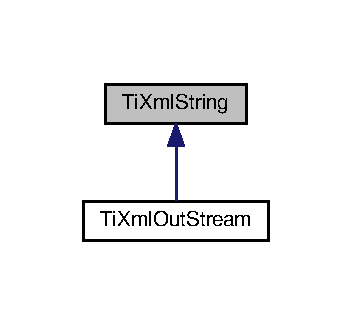
\includegraphics[width=169pt]{classTiXmlString__inherit__graph}
\end{center}
\end{figure}
\subsection*{Public Types}
\begin{DoxyCompactItemize}
\item 
typedef size\+\_\+t {\bfseries size\+\_\+type}\hypertarget{classTiXmlString_abeb2c1893a04c17904f7c06546d0b971}{}\label{classTiXmlString_abeb2c1893a04c17904f7c06546d0b971}

\end{DoxyCompactItemize}
\subsection*{Public Member Functions}
\begin{DoxyCompactItemize}
\item 
{\bfseries Ti\+Xml\+String} (const \hyperlink{classTiXmlString}{Ti\+Xml\+String} \&copy)\hypertarget{classTiXmlString_ac80fe17693a438c9ab2591664743fcb6}{}\label{classTiXmlString_ac80fe17693a438c9ab2591664743fcb6}

\item 
T\+I\+X\+M\+L\+\_\+\+E\+X\+P\+L\+I\+C\+IT {\bfseries Ti\+Xml\+String} (const char $\ast$copy)\hypertarget{classTiXmlString_aa3b32bd2891a757c9f36c21db44c81d2}{}\label{classTiXmlString_aa3b32bd2891a757c9f36c21db44c81d2}

\item 
T\+I\+X\+M\+L\+\_\+\+E\+X\+P\+L\+I\+C\+IT {\bfseries Ti\+Xml\+String} (const char $\ast$str, size\+\_\+type len)\hypertarget{classTiXmlString_a4b17ea5c5db986f14827223dfa8f1547}{}\label{classTiXmlString_a4b17ea5c5db986f14827223dfa8f1547}

\item 
\hyperlink{classTiXmlString}{Ti\+Xml\+String} \& {\bfseries operator=} (const char $\ast$copy)\hypertarget{classTiXmlString_ae0bc6147afc0ec2aa0da3a3c0a8fcfb0}{}\label{classTiXmlString_ae0bc6147afc0ec2aa0da3a3c0a8fcfb0}

\item 
\hyperlink{classTiXmlString}{Ti\+Xml\+String} \& {\bfseries operator=} (const \hyperlink{classTiXmlString}{Ti\+Xml\+String} \&copy)\hypertarget{classTiXmlString_ab1f1f5d3eceaa0f22d0a7e6055ea81b0}{}\label{classTiXmlString_ab1f1f5d3eceaa0f22d0a7e6055ea81b0}

\item 
\hyperlink{classTiXmlString}{Ti\+Xml\+String} \& {\bfseries operator+=} (const char $\ast$suffix)\hypertarget{classTiXmlString_ab56336ac2aa2a08d24a71eb9a2b502a5}{}\label{classTiXmlString_ab56336ac2aa2a08d24a71eb9a2b502a5}

\item 
\hyperlink{classTiXmlString}{Ti\+Xml\+String} \& {\bfseries operator+=} (char single)\hypertarget{classTiXmlString_a6aa09d5240470b76d54ec709e04f8c13}{}\label{classTiXmlString_a6aa09d5240470b76d54ec709e04f8c13}

\item 
\hyperlink{classTiXmlString}{Ti\+Xml\+String} \& {\bfseries operator+=} (const \hyperlink{classTiXmlString}{Ti\+Xml\+String} \&suffix)\hypertarget{classTiXmlString_afdcae5ea2b4d9e194dc21226b817f417}{}\label{classTiXmlString_afdcae5ea2b4d9e194dc21226b817f417}

\item 
const char $\ast$ {\bfseries c\+\_\+str} () const \hypertarget{classTiXmlString_a5581ca641d915551d3cda90f8e7bf49b}{}\label{classTiXmlString_a5581ca641d915551d3cda90f8e7bf49b}

\item 
const char $\ast$ {\bfseries data} () const \hypertarget{classTiXmlString_a00abc60f135c7ca1951c7334cc2c7993}{}\label{classTiXmlString_a00abc60f135c7ca1951c7334cc2c7993}

\item 
size\+\_\+type {\bfseries length} () const \hypertarget{classTiXmlString_a3202f27d139a3fac79205f1f3c707727}{}\label{classTiXmlString_a3202f27d139a3fac79205f1f3c707727}

\item 
size\+\_\+type {\bfseries size} () const \hypertarget{classTiXmlString_a96103e5c0f67e987fa48527e1f47a1f6}{}\label{classTiXmlString_a96103e5c0f67e987fa48527e1f47a1f6}

\item 
bool {\bfseries empty} () const \hypertarget{classTiXmlString_a9a61e1d11cdb71bea4a4ed79caa793f4}{}\label{classTiXmlString_a9a61e1d11cdb71bea4a4ed79caa793f4}

\item 
size\+\_\+type {\bfseries capacity} () const \hypertarget{classTiXmlString_a76e4d6aba7845f4cf9c02332a5fbf916}{}\label{classTiXmlString_a76e4d6aba7845f4cf9c02332a5fbf916}

\item 
const char \& {\bfseries at} (size\+\_\+type index) const \hypertarget{classTiXmlString_a6763093267bbdecbf03f8840bc349877}{}\label{classTiXmlString_a6763093267bbdecbf03f8840bc349877}

\item 
char \& {\bfseries operator\mbox{[}$\,$\mbox{]}} (size\+\_\+type index) const \hypertarget{classTiXmlString_ae8cdc1d46c538536b786f7ae03c0c1d9}{}\label{classTiXmlString_ae8cdc1d46c538536b786f7ae03c0c1d9}

\item 
size\+\_\+type {\bfseries find} (char lookup) const \hypertarget{classTiXmlString_a5c2b368b5eafe075fd9565cbcbd4c2f9}{}\label{classTiXmlString_a5c2b368b5eafe075fd9565cbcbd4c2f9}

\item 
size\+\_\+type {\bfseries find} (char tofind, size\+\_\+type offset) const \hypertarget{classTiXmlString_a5f2a6fd565751410b392f249a9786db4}{}\label{classTiXmlString_a5f2a6fd565751410b392f249a9786db4}

\item 
void {\bfseries clear} ()\hypertarget{classTiXmlString_ab20e06e4c666abf3bdbfb3a1191d4888}{}\label{classTiXmlString_ab20e06e4c666abf3bdbfb3a1191d4888}

\item 
void {\bfseries reserve} (size\+\_\+type cap)\hypertarget{classTiXmlString_a88ecf9f0f00cb5c67b6b637958d7049c}{}\label{classTiXmlString_a88ecf9f0f00cb5c67b6b637958d7049c}

\item 
\hyperlink{classTiXmlString}{Ti\+Xml\+String} \& {\bfseries assign} (const char $\ast$str, size\+\_\+type len)\hypertarget{classTiXmlString_ac72f3d9149b7812c1e6c59402014d0d5}{}\label{classTiXmlString_ac72f3d9149b7812c1e6c59402014d0d5}

\item 
\hyperlink{classTiXmlString}{Ti\+Xml\+String} \& {\bfseries append} (const char $\ast$str, size\+\_\+type len)\hypertarget{classTiXmlString_ad44b21700d2ec24a511367b222b643fb}{}\label{classTiXmlString_ad44b21700d2ec24a511367b222b643fb}

\item 
void {\bfseries swap} (\hyperlink{classTiXmlString}{Ti\+Xml\+String} \&other)\hypertarget{classTiXmlString_aa392cbc180752a79f007f4f9280c7762}{}\label{classTiXmlString_aa392cbc180752a79f007f4f9280c7762}

\end{DoxyCompactItemize}
\subsection*{Static Public Attributes}
\begin{DoxyCompactItemize}
\item 
static const size\+\_\+type {\bfseries npos} = static\+\_\+cast$<$ Ti\+Xml\+String\+::size\+\_\+type $>$(-\/1)\hypertarget{classTiXmlString_a8f4422d227088dc7bec96f479b275d0a}{}\label{classTiXmlString_a8f4422d227088dc7bec96f479b275d0a}

\end{DoxyCompactItemize}


The documentation for this class was generated from the following files\+:\begin{DoxyCompactItemize}
\item 
src/tinyxml/tinystr.\+h\item 
src/tinyxml/tinystr.\+cpp\end{DoxyCompactItemize}

\hypertarget{classTiXmlText}{}\section{Ti\+Xml\+Text Class Reference}
\label{classTiXmlText}\index{Ti\+Xml\+Text@{Ti\+Xml\+Text}}


{\ttfamily \#include $<$tinyxml.\+h$>$}



Inheritance diagram for Ti\+Xml\+Text\+:\nopagebreak
\begin{figure}[H]
\begin{center}
\leavevmode
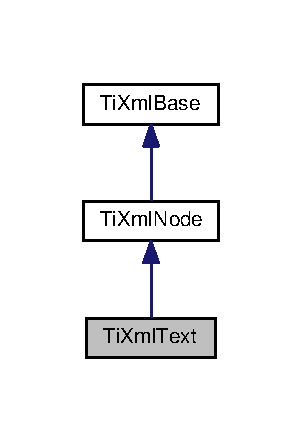
\includegraphics[width=145pt]{classTiXmlText__inherit__graph}
\end{center}
\end{figure}


Collaboration diagram for Ti\+Xml\+Text\+:\nopagebreak
\begin{figure}[H]
\begin{center}
\leavevmode
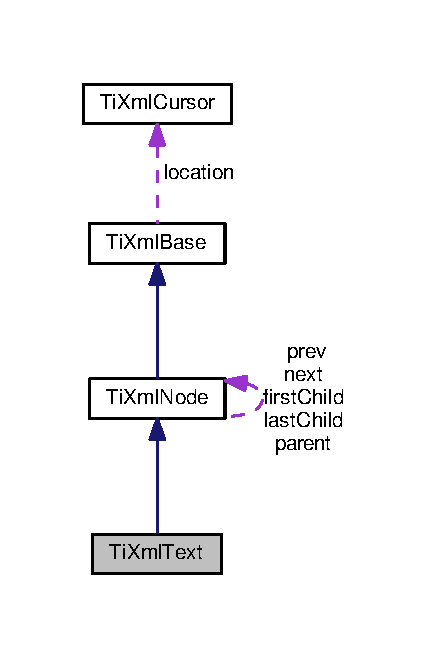
\includegraphics[width=206pt]{classTiXmlText__coll__graph}
\end{center}
\end{figure}
\subsection*{Public Member Functions}
\begin{DoxyCompactItemize}
\item 
\hyperlink{classTiXmlText_af659e77c6b87d684827f35a8f4895960}{Ti\+Xml\+Text} (const char $\ast$init\+Value)
\item 
{\bfseries Ti\+Xml\+Text} (const \hyperlink{classTiXmlText}{Ti\+Xml\+Text} \&copy)\hypertarget{classTiXmlText_a8d2cc1b4af2208cbb0171cf20f6815d1}{}\label{classTiXmlText_a8d2cc1b4af2208cbb0171cf20f6815d1}

\item 
\hyperlink{classTiXmlText}{Ti\+Xml\+Text} \& {\bfseries operator=} (const \hyperlink{classTiXmlText}{Ti\+Xml\+Text} \&base)\hypertarget{classTiXmlText_aed5b13f9c1b804c616fd533882c29f57}{}\label{classTiXmlText_aed5b13f9c1b804c616fd533882c29f57}

\item 
virtual void \hyperlink{classTiXmlText_ae74d56c5b3ddec6cc3103dd51821af92}{Print} (F\+I\+LE $\ast$cfile, int depth) const 
\item 
bool \hyperlink{classTiXmlText_ad1a6a6b83fa2271022dd97c072a2b586}{C\+D\+A\+TA} () const \hypertarget{classTiXmlText_ad1a6a6b83fa2271022dd97c072a2b586}{}\label{classTiXmlText_ad1a6a6b83fa2271022dd97c072a2b586}

\begin{DoxyCompactList}\small\item\em Queries whether this represents text using a C\+D\+A\+TA section. \end{DoxyCompactList}\item 
void \hyperlink{classTiXmlText_acb17ff7c5d09b2c839393445a3de5ea9}{Set\+C\+D\+A\+TA} (bool \+\_\+cdata)\hypertarget{classTiXmlText_acb17ff7c5d09b2c839393445a3de5ea9}{}\label{classTiXmlText_acb17ff7c5d09b2c839393445a3de5ea9}

\begin{DoxyCompactList}\small\item\em Turns on or off a C\+D\+A\+TA representation of text. \end{DoxyCompactList}\item 
virtual const char $\ast$ {\bfseries Parse} (const char $\ast$p, \hyperlink{classTiXmlParsingData}{Ti\+Xml\+Parsing\+Data} $\ast$data, Ti\+Xml\+Encoding encoding)\hypertarget{classTiXmlText_a8d2dcfa41fc73d3e62dacc2fcf633819}{}\label{classTiXmlText_a8d2dcfa41fc73d3e62dacc2fcf633819}

\item 
virtual const \hyperlink{classTiXmlText}{Ti\+Xml\+Text} $\ast$ \hyperlink{classTiXmlText_a895bf34ffad17f7439ab2a52b9651648}{To\+Text} () const \hypertarget{classTiXmlText_a895bf34ffad17f7439ab2a52b9651648}{}\label{classTiXmlText_a895bf34ffad17f7439ab2a52b9651648}

\begin{DoxyCompactList}\small\item\em Cast to a more defined type. Will return null not of the requested type. \end{DoxyCompactList}\item 
virtual \hyperlink{classTiXmlText}{Ti\+Xml\+Text} $\ast$ \hyperlink{classTiXmlText_ae7c3a8fd3e4dbf6c0c4363a943d72f5b}{To\+Text} ()\hypertarget{classTiXmlText_ae7c3a8fd3e4dbf6c0c4363a943d72f5b}{}\label{classTiXmlText_ae7c3a8fd3e4dbf6c0c4363a943d72f5b}

\begin{DoxyCompactList}\small\item\em Cast to a more defined type. Will return null not of the requested type. \end{DoxyCompactList}\item 
virtual bool \hyperlink{classTiXmlText_a43b9954ebf679557fac1a4453f337b7c}{Accept} (\hyperlink{classTiXmlVisitor}{Ti\+Xml\+Visitor} $\ast$content) const 
\end{DoxyCompactItemize}
\subsection*{Protected Member Functions}
\begin{DoxyCompactItemize}
\item 
virtual \hyperlink{classTiXmlNode}{Ti\+Xml\+Node} $\ast$ \hyperlink{classTiXmlText_adde1869dfb029be50713fbfd8ce4d21f}{Clone} () const \hypertarget{classTiXmlText_adde1869dfb029be50713fbfd8ce4d21f}{}\label{classTiXmlText_adde1869dfb029be50713fbfd8ce4d21f}

\begin{DoxyCompactList}\small\item\em \mbox{[}internal use\mbox{]} Creates a new Element and returns it. \end{DoxyCompactList}\item 
void {\bfseries Copy\+To} (\hyperlink{classTiXmlText}{Ti\+Xml\+Text} $\ast$target) const \hypertarget{classTiXmlText_adcec7d9b6fccfc5777452bb97e6031c1}{}\label{classTiXmlText_adcec7d9b6fccfc5777452bb97e6031c1}

\item 
bool {\bfseries Blank} () const \hypertarget{classTiXmlText_a1c120428e3b3cf24d79706e6d2b65aa6}{}\label{classTiXmlText_a1c120428e3b3cf24d79706e6d2b65aa6}

\end{DoxyCompactItemize}
\subsection*{Friends}
\begin{DoxyCompactItemize}
\item 
class {\bfseries Ti\+Xml\+Element}\hypertarget{classTiXmlText_ab6592e32cb9132be517cc12a70564c4b}{}\label{classTiXmlText_ab6592e32cb9132be517cc12a70564c4b}

\end{DoxyCompactItemize}
\subsection*{Additional Inherited Members}


\subsection{Detailed Description}
X\+ML text. A text node can have 2 ways to output the next. \char`\"{}normal\char`\"{} output and C\+D\+A\+TA. It will default to the mode it was parsed from the X\+ML file and you generally want to leave it alone, but you can change the output mode with \hyperlink{classTiXmlText_acb17ff7c5d09b2c839393445a3de5ea9}{Set\+C\+D\+A\+T\+A()} and query it with \hyperlink{classTiXmlText_ad1a6a6b83fa2271022dd97c072a2b586}{C\+D\+A\+T\+A()}. 

\subsection{Constructor \& Destructor Documentation}
\index{Ti\+Xml\+Text@{Ti\+Xml\+Text}!Ti\+Xml\+Text@{Ti\+Xml\+Text}}
\index{Ti\+Xml\+Text@{Ti\+Xml\+Text}!Ti\+Xml\+Text@{Ti\+Xml\+Text}}
\subsubsection[{\texorpdfstring{Ti\+Xml\+Text(const char $\ast$init\+Value)}{TiXmlText(const char *initValue)}}]{\setlength{\rightskip}{0pt plus 5cm}Ti\+Xml\+Text\+::\+Ti\+Xml\+Text (
\begin{DoxyParamCaption}
\item[{const char $\ast$}]{init\+Value}
\end{DoxyParamCaption}
)\hspace{0.3cm}{\ttfamily [inline]}}\hypertarget{classTiXmlText_af659e77c6b87d684827f35a8f4895960}{}\label{classTiXmlText_af659e77c6b87d684827f35a8f4895960}
Constructor for text element. By default, it is treated as normal, encoded text. If you want it be output as a C\+D\+A\+TA text element, set the parameter \+\_\+cdata to \textquotesingle{}true\textquotesingle{} 

\subsection{Member Function Documentation}
\index{Ti\+Xml\+Text@{Ti\+Xml\+Text}!Accept@{Accept}}
\index{Accept@{Accept}!Ti\+Xml\+Text@{Ti\+Xml\+Text}}
\subsubsection[{\texorpdfstring{Accept(\+Ti\+Xml\+Visitor $\ast$content) const }{Accept(TiXmlVisitor *content) const }}]{\setlength{\rightskip}{0pt plus 5cm}bool Ti\+Xml\+Text\+::\+Accept (
\begin{DoxyParamCaption}
\item[{{\bf Ti\+Xml\+Visitor} $\ast$}]{content}
\end{DoxyParamCaption}
) const\hspace{0.3cm}{\ttfamily [virtual]}}\hypertarget{classTiXmlText_a43b9954ebf679557fac1a4453f337b7c}{}\label{classTiXmlText_a43b9954ebf679557fac1a4453f337b7c}
Walk the X\+ML tree visiting this node and all of its children. 

Implements \hyperlink{classTiXmlNode_acc0f88b7462c6cb73809d410a4f5bb86}{Ti\+Xml\+Node}.

\index{Ti\+Xml\+Text@{Ti\+Xml\+Text}!Print@{Print}}
\index{Print@{Print}!Ti\+Xml\+Text@{Ti\+Xml\+Text}}
\subsubsection[{\texorpdfstring{Print(\+F\+I\+L\+E $\ast$cfile, int depth) const }{Print(FILE *cfile, int depth) const }}]{\setlength{\rightskip}{0pt plus 5cm}void Ti\+Xml\+Text\+::\+Print (
\begin{DoxyParamCaption}
\item[{F\+I\+LE $\ast$}]{cfile, }
\item[{int}]{depth}
\end{DoxyParamCaption}
) const\hspace{0.3cm}{\ttfamily [virtual]}}\hypertarget{classTiXmlText_ae74d56c5b3ddec6cc3103dd51821af92}{}\label{classTiXmlText_ae74d56c5b3ddec6cc3103dd51821af92}
All Tiny\+Xml classes can print themselves to a filestream or the string class (\hyperlink{classTiXmlString}{Ti\+Xml\+String} in non-\/\+S\+TL mode, std\+::string in S\+TL mode.) Either or both cfile and str can be null.

This is a formatted print, and will insert tabs and newlines.

(For an unformatted stream, use the $<$$<$ operator.) 

Implements \hyperlink{classTiXmlBase_a0de56b3f2ef14c65091a3b916437b512}{Ti\+Xml\+Base}.



The documentation for this class was generated from the following files\+:\begin{DoxyCompactItemize}
\item 
src/tinyxml/tinyxml.\+h\item 
src/tinyxml/tinyxml.\+cpp\item 
src/tinyxml/tinyxmlparser.\+cpp\end{DoxyCompactItemize}

\hypertarget{classTiXmlUnknown}{}\section{Ti\+Xml\+Unknown Class Reference}
\label{classTiXmlUnknown}\index{Ti\+Xml\+Unknown@{Ti\+Xml\+Unknown}}


{\ttfamily \#include $<$tinyxml.\+h$>$}



Inheritance diagram for Ti\+Xml\+Unknown\+:\nopagebreak
\begin{figure}[H]
\begin{center}
\leavevmode
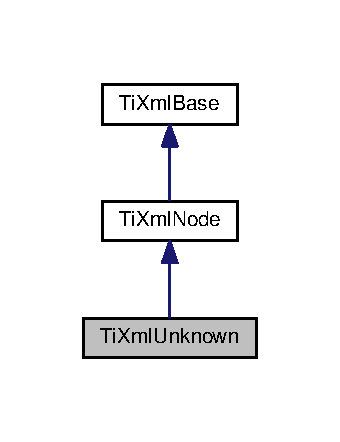
\includegraphics[width=163pt]{classTiXmlUnknown__inherit__graph}
\end{center}
\end{figure}


Collaboration diagram for Ti\+Xml\+Unknown\+:\nopagebreak
\begin{figure}[H]
\begin{center}
\leavevmode
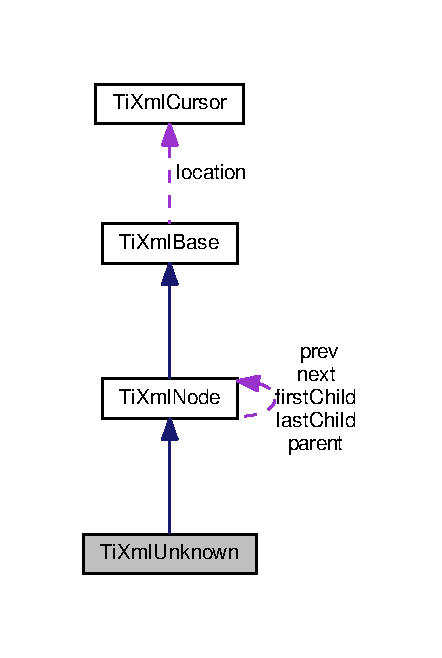
\includegraphics[width=212pt]{classTiXmlUnknown__coll__graph}
\end{center}
\end{figure}
\subsection*{Public Member Functions}
\begin{DoxyCompactItemize}
\item 
{\bfseries Ti\+Xml\+Unknown} (const \hyperlink{classTiXmlUnknown}{Ti\+Xml\+Unknown} \&copy)\hypertarget{classTiXmlUnknown_abe798ff4feea31474850c7f0de6bdf5e}{}\label{classTiXmlUnknown_abe798ff4feea31474850c7f0de6bdf5e}

\item 
\hyperlink{classTiXmlUnknown}{Ti\+Xml\+Unknown} \& {\bfseries operator=} (const \hyperlink{classTiXmlUnknown}{Ti\+Xml\+Unknown} \&copy)\hypertarget{classTiXmlUnknown_a60560b5aacb4bdc8b2b5f02f0a99c5c0}{}\label{classTiXmlUnknown_a60560b5aacb4bdc8b2b5f02f0a99c5c0}

\item 
virtual \hyperlink{classTiXmlNode}{Ti\+Xml\+Node} $\ast$ \hyperlink{classTiXmlUnknown_a675c4b2684af35e4c7649b7fd5ae598d}{Clone} () const \hypertarget{classTiXmlUnknown_a675c4b2684af35e4c7649b7fd5ae598d}{}\label{classTiXmlUnknown_a675c4b2684af35e4c7649b7fd5ae598d}

\begin{DoxyCompactList}\small\item\em Creates a copy of this Unknown and returns it. \end{DoxyCompactList}\item 
virtual void \hyperlink{classTiXmlUnknown_a025f19c21ef01ea9be50febb8fe0ba06}{Print} (F\+I\+LE $\ast$cfile, int depth) const 
\item 
virtual const char $\ast$ {\bfseries Parse} (const char $\ast$p, \hyperlink{classTiXmlParsingData}{Ti\+Xml\+Parsing\+Data} $\ast$data, Ti\+Xml\+Encoding encoding)\hypertarget{classTiXmlUnknown_aa51c2694e4177b5f0b5429ee5a81b58d}{}\label{classTiXmlUnknown_aa51c2694e4177b5f0b5429ee5a81b58d}

\item 
virtual const \hyperlink{classTiXmlUnknown}{Ti\+Xml\+Unknown} $\ast$ \hyperlink{classTiXmlUnknown_ab0313e5fe77987d746ac1a97a254419d}{To\+Unknown} () const \hypertarget{classTiXmlUnknown_ab0313e5fe77987d746ac1a97a254419d}{}\label{classTiXmlUnknown_ab0313e5fe77987d746ac1a97a254419d}

\begin{DoxyCompactList}\small\item\em Cast to a more defined type. Will return null not of the requested type. \end{DoxyCompactList}\item 
virtual \hyperlink{classTiXmlUnknown}{Ti\+Xml\+Unknown} $\ast$ \hyperlink{classTiXmlUnknown_a67c9fd22940e8c47f706a72cdd2e332c}{To\+Unknown} ()\hypertarget{classTiXmlUnknown_a67c9fd22940e8c47f706a72cdd2e332c}{}\label{classTiXmlUnknown_a67c9fd22940e8c47f706a72cdd2e332c}

\begin{DoxyCompactList}\small\item\em Cast to a more defined type. Will return null not of the requested type. \end{DoxyCompactList}\item 
virtual bool \hyperlink{classTiXmlUnknown_a4e54d7482e05a837cf83c925cc683380}{Accept} (\hyperlink{classTiXmlVisitor}{Ti\+Xml\+Visitor} $\ast$content) const 
\end{DoxyCompactItemize}
\subsection*{Protected Member Functions}
\begin{DoxyCompactItemize}
\item 
void {\bfseries Copy\+To} (\hyperlink{classTiXmlUnknown}{Ti\+Xml\+Unknown} $\ast$target) const \hypertarget{classTiXmlUnknown_a08ca7b225a2bcb604d3c72e199d33408}{}\label{classTiXmlUnknown_a08ca7b225a2bcb604d3c72e199d33408}

\end{DoxyCompactItemize}
\subsection*{Additional Inherited Members}


\subsection{Detailed Description}
Any tag that tiny\+Xml doesn\textquotesingle{}t recognize is saved as an unknown. It is a tag of text, but should not be modified. It will be written back to the X\+ML, unchanged, when the file is saved.

D\+TD tags get thrown into Ti\+Xml\+Unknowns. 

\subsection{Member Function Documentation}
\index{Ti\+Xml\+Unknown@{Ti\+Xml\+Unknown}!Accept@{Accept}}
\index{Accept@{Accept}!Ti\+Xml\+Unknown@{Ti\+Xml\+Unknown}}
\subsubsection[{\texorpdfstring{Accept(\+Ti\+Xml\+Visitor $\ast$content) const }{Accept(TiXmlVisitor *content) const }}]{\setlength{\rightskip}{0pt plus 5cm}bool Ti\+Xml\+Unknown\+::\+Accept (
\begin{DoxyParamCaption}
\item[{{\bf Ti\+Xml\+Visitor} $\ast$}]{content}
\end{DoxyParamCaption}
) const\hspace{0.3cm}{\ttfamily [virtual]}}\hypertarget{classTiXmlUnknown_a4e54d7482e05a837cf83c925cc683380}{}\label{classTiXmlUnknown_a4e54d7482e05a837cf83c925cc683380}
Walk the X\+ML tree visiting this node and all of its children. 

Implements \hyperlink{classTiXmlNode_acc0f88b7462c6cb73809d410a4f5bb86}{Ti\+Xml\+Node}.

\index{Ti\+Xml\+Unknown@{Ti\+Xml\+Unknown}!Print@{Print}}
\index{Print@{Print}!Ti\+Xml\+Unknown@{Ti\+Xml\+Unknown}}
\subsubsection[{\texorpdfstring{Print(\+F\+I\+L\+E $\ast$cfile, int depth) const }{Print(FILE *cfile, int depth) const }}]{\setlength{\rightskip}{0pt plus 5cm}void Ti\+Xml\+Unknown\+::\+Print (
\begin{DoxyParamCaption}
\item[{F\+I\+LE $\ast$}]{cfile, }
\item[{int}]{depth}
\end{DoxyParamCaption}
) const\hspace{0.3cm}{\ttfamily [virtual]}}\hypertarget{classTiXmlUnknown_a025f19c21ef01ea9be50febb8fe0ba06}{}\label{classTiXmlUnknown_a025f19c21ef01ea9be50febb8fe0ba06}
All Tiny\+Xml classes can print themselves to a filestream or the string class (\hyperlink{classTiXmlString}{Ti\+Xml\+String} in non-\/\+S\+TL mode, std\+::string in S\+TL mode.) Either or both cfile and str can be null.

This is a formatted print, and will insert tabs and newlines.

(For an unformatted stream, use the $<$$<$ operator.) 

Implements \hyperlink{classTiXmlBase_a0de56b3f2ef14c65091a3b916437b512}{Ti\+Xml\+Base}.



The documentation for this class was generated from the following files\+:\begin{DoxyCompactItemize}
\item 
src/tinyxml.\+h\item 
src/tinyxml.\+cpp\item 
src/tinyxmlparser.\+cpp\end{DoxyCompactItemize}

\hypertarget{classTiXmlVisitor}{}\section{Ti\+Xml\+Visitor Class Reference}
\label{classTiXmlVisitor}\index{Ti\+Xml\+Visitor@{Ti\+Xml\+Visitor}}


{\ttfamily \#include $<$tinyxml.\+h$>$}



Inheritance diagram for Ti\+Xml\+Visitor\+:\nopagebreak
\begin{figure}[H]
\begin{center}
\leavevmode
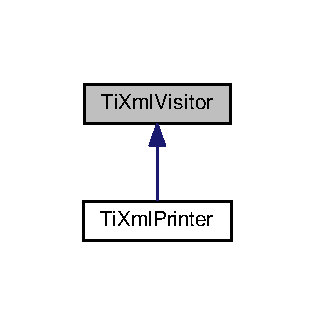
\includegraphics[width=151pt]{classTiXmlVisitor__inherit__graph}
\end{center}
\end{figure}
\subsection*{Public Member Functions}
\begin{DoxyCompactItemize}
\item 
virtual bool \hyperlink{classTiXmlVisitor_a07baecb52dd7d8716ae2a48ad0956ee0}{Visit\+Enter} (const \hyperlink{classTiXmlDocument}{Ti\+Xml\+Document} \&)\hypertarget{classTiXmlVisitor_a07baecb52dd7d8716ae2a48ad0956ee0}{}\label{classTiXmlVisitor_a07baecb52dd7d8716ae2a48ad0956ee0}

\begin{DoxyCompactList}\small\item\em Visit a document. \end{DoxyCompactList}\item 
virtual bool \hyperlink{classTiXmlVisitor_aa0ade4f27087447e93974e975c3246ad}{Visit\+Exit} (const \hyperlink{classTiXmlDocument}{Ti\+Xml\+Document} \&)\hypertarget{classTiXmlVisitor_aa0ade4f27087447e93974e975c3246ad}{}\label{classTiXmlVisitor_aa0ade4f27087447e93974e975c3246ad}

\begin{DoxyCompactList}\small\item\em Visit a document. \end{DoxyCompactList}\item 
virtual bool \hyperlink{classTiXmlVisitor_af6c6178ffa517bbdba95d70490875fff}{Visit\+Enter} (const \hyperlink{classTiXmlElement}{Ti\+Xml\+Element} \&, const \hyperlink{classTiXmlAttribute}{Ti\+Xml\+Attribute} $\ast$)\hypertarget{classTiXmlVisitor_af6c6178ffa517bbdba95d70490875fff}{}\label{classTiXmlVisitor_af6c6178ffa517bbdba95d70490875fff}

\begin{DoxyCompactList}\small\item\em Visit an element. \end{DoxyCompactList}\item 
virtual bool \hyperlink{classTiXmlVisitor_aec2b1f8116226d52f3a1b95dafd3a32c}{Visit\+Exit} (const \hyperlink{classTiXmlElement}{Ti\+Xml\+Element} \&)\hypertarget{classTiXmlVisitor_aec2b1f8116226d52f3a1b95dafd3a32c}{}\label{classTiXmlVisitor_aec2b1f8116226d52f3a1b95dafd3a32c}

\begin{DoxyCompactList}\small\item\em Visit an element. \end{DoxyCompactList}\item 
virtual bool \hyperlink{classTiXmlVisitor_afad71c71ce6473fb9b4b64cd92de4a19}{Visit} (const \hyperlink{classTiXmlDeclaration}{Ti\+Xml\+Declaration} \&)\hypertarget{classTiXmlVisitor_afad71c71ce6473fb9b4b64cd92de4a19}{}\label{classTiXmlVisitor_afad71c71ce6473fb9b4b64cd92de4a19}

\begin{DoxyCompactList}\small\item\em Visit a declaration. \end{DoxyCompactList}\item 
virtual bool \hyperlink{classTiXmlVisitor_a399b8ebca5cd14664974a32d2ce029e5}{Visit} (const \hyperlink{classTiXmlText}{Ti\+Xml\+Text} \&)\hypertarget{classTiXmlVisitor_a399b8ebca5cd14664974a32d2ce029e5}{}\label{classTiXmlVisitor_a399b8ebca5cd14664974a32d2ce029e5}

\begin{DoxyCompactList}\small\item\em Visit a text node. \end{DoxyCompactList}\item 
virtual bool \hyperlink{classTiXmlVisitor_a53a60e7a528627b31af3161972cc7fa2}{Visit} (const \hyperlink{classTiXmlComment}{Ti\+Xml\+Comment} \&)\hypertarget{classTiXmlVisitor_a53a60e7a528627b31af3161972cc7fa2}{}\label{classTiXmlVisitor_a53a60e7a528627b31af3161972cc7fa2}

\begin{DoxyCompactList}\small\item\em Visit a comment node. \end{DoxyCompactList}\item 
virtual bool \hyperlink{classTiXmlVisitor_a7e284d607d275c51dac1adb58159ce28}{Visit} (const \hyperlink{classTiXmlUnknown}{Ti\+Xml\+Unknown} \&)\hypertarget{classTiXmlVisitor_a7e284d607d275c51dac1adb58159ce28}{}\label{classTiXmlVisitor_a7e284d607d275c51dac1adb58159ce28}

\begin{DoxyCompactList}\small\item\em Visit an unknown node. \end{DoxyCompactList}\end{DoxyCompactItemize}


\subsection{Detailed Description}
Implements the interface to the \char`\"{}\+Visitor pattern\char`\"{} (see the Accept() method.) If you call the Accept() method, it requires being passed a \hyperlink{classTiXmlVisitor}{Ti\+Xml\+Visitor} class to handle callbacks. For nodes that contain other nodes (Document, Element) you will get called with a Visit\+Enter/\+Visit\+Exit pair. Nodes that are always leaves are simply called with \hyperlink{classTiXmlVisitor_afad71c71ce6473fb9b4b64cd92de4a19}{Visit()}.

If you return \textquotesingle{}true\textquotesingle{} from a Visit method, recursive parsing will continue. If you return false, {\bfseries no children of this node or its sibilings} will be Visited.

All flavors of Visit methods have a default implementation that returns \textquotesingle{}true\textquotesingle{} (continue visiting). You need to only override methods that are interesting to you.

Generally Accept() is called on the \hyperlink{classTiXmlDocument}{Ti\+Xml\+Document}, although all nodes suppert Visiting.

You should never change the document from a callback.

\begin{DoxySeeAlso}{See also}
\hyperlink{classTiXmlNode_acc0f88b7462c6cb73809d410a4f5bb86}{Ti\+Xml\+Node\+::\+Accept()} 
\end{DoxySeeAlso}


The documentation for this class was generated from the following file\+:\begin{DoxyCompactItemize}
\item 
src/tinyxml.\+h\end{DoxyCompactItemize}

\hypertarget{classTram}{}\section{Tram Class Reference}
\label{classTram}\index{Tram@{Tram}}


This Class contains all the functionalities for the \hyperlink{classTram}{Tram} objects.  




{\ttfamily \#include $<$Tram.\+h$>$}

\subsection*{Public Member Functions}
\begin{DoxyCompactItemize}
\item 
\hyperlink{classTram_aad83b2e7e79d57528691bf317ab0e1ef}{Tram} ()
\begin{DoxyCompactList}\small\item\em \hyperlink{classTram}{Tram} Default Constructor. \end{DoxyCompactList}\item 
int \hyperlink{classTram_ab5a70cf696779f9dff401244e203f6c8}{get\+Lijn\+Nr} ()
\begin{DoxyCompactList}\small\item\em Returns the \hyperlink{classTram}{Tram} object\textquotesingle{}s Line Number. \end{DoxyCompactList}\item 
int \hyperlink{classTram_a018207b3cd1f01821b5f64e4f4f394a5}{get\+Zitplaatsen} ()
\begin{DoxyCompactList}\small\item\em Returns the \hyperlink{classTram}{Tram} object\textquotesingle{}s Amount of Seats. \end{DoxyCompactList}\item 
int \hyperlink{classTram_afcd79d44b9bc18fb1e7302daa40f56f5}{get\+Snelheid} ()
\begin{DoxyCompactList}\small\item\em Returns the \hyperlink{classTram}{Tram} object\textquotesingle{}s Speed. \end{DoxyCompactList}\item 
string \hyperlink{classTram_a0d61611abd4dc61f3fbad6b4b7bc6403}{get\+Begin\+Station} ()
\begin{DoxyCompactList}\small\item\em Returns the \hyperlink{classTram}{Tram} object\textquotesingle{}s Starting \hyperlink{classStation}{Station}. \end{DoxyCompactList}\item 
string \hyperlink{classTram_a1e28b662a6ef3833faa2920247a139ee}{get\+Huidig\+Station} ()
\begin{DoxyCompactList}\small\item\em Returns the Passenger object\textquotesingle{}s Current \hyperlink{classStation}{Station}. \end{DoxyCompactList}\item 
int \hyperlink{classTram_abce34b0915945a2d7ede17297a727301}{get\+Voertuig\+Nr} ()
\begin{DoxyCompactList}\small\item\em Returns the \hyperlink{classTram}{Tram} object\textquotesingle{}s Vehicle Number. \end{DoxyCompactList}\item 
void \hyperlink{classTram_ac877b48ea6699c11ae580d8c71e140ac}{set\+Lijn\+Nr} (int lijn\+Nr)
\begin{DoxyCompactList}\small\item\em Sets a new \hyperlink{classTram}{Tram} object\textquotesingle{}s Line Number. \end{DoxyCompactList}\item 
void \hyperlink{classTram_a9071e3ddf218c290ae5d7ef3365097eb}{set\+Zitplaatsen} (int zitplaatsen)
\begin{DoxyCompactList}\small\item\em Sets a new \hyperlink{classTram}{Tram} object\textquotesingle{}s Amount of Seats. \end{DoxyCompactList}\item 
void \hyperlink{classTram_a2853d9b5d5d519e6757e6e3480d3b1c6}{set\+Snelheid} (int snelheid)
\begin{DoxyCompactList}\small\item\em Sets a new \hyperlink{classTram}{Tram} object\textquotesingle{}s Speed. \end{DoxyCompactList}\item 
void \hyperlink{classTram_a1f940f1fa5c8be660561f24750f25dd7}{set\+Begin\+Station} (string begin\+Station)
\begin{DoxyCompactList}\small\item\em Sets a new Passenger object\textquotesingle{}s Starting \hyperlink{classStation}{Station}. \end{DoxyCompactList}\item 
void \hyperlink{classTram_a3db658161102fcd0eccf7975982b1f1d}{set\+Huidig\+Station} (string huidig\+Station)
\begin{DoxyCompactList}\small\item\em Sets a new Passenger object\textquotesingle{}s Starting \hyperlink{classStation}{Station}. \end{DoxyCompactList}\item 
void \hyperlink{classTram_a4912c2cd70ee32329220618068c28692}{set\+Voertuig\+Nr} (int voertuig\+Nr)
\begin{DoxyCompactList}\small\item\em Sets a new \hyperlink{classTram}{Tram} Object. \end{DoxyCompactList}\item 
bool \hyperlink{classTram_ac69cbbacaed7e1b9e60e608d766d02ee}{properly\+Initialized} ()
\begin{DoxyCompactList}\small\item\em Returns true if properly initialized, false if not. \end{DoxyCompactList}\item 
bool \hyperlink{classTram_acbd3c261e6b3830741de4e37643cc9cf}{plaatsen\+Te\+Kort} (int aantal)
\begin{DoxyCompactList}\small\item\em Returns true if there\textquotesingle{}s enough seats available on the \hyperlink{classTram}{Tram}. \end{DoxyCompactList}\item 
string {\bfseries add\+Passagiers} (string \hyperlink{classPassagier}{Passagier}, int Aantal, string \hyperlink{classStation}{Station})\hypertarget{classTram_a27f0c6832da5869a5173cc440fec9719}{}\label{classTram_a27f0c6832da5869a5173cc440fec9719}

\item 
string {\bfseries remove\+Passagiers} (string, int, string)\hypertarget{classTram_aefa8209a2667b653b56b0c48c801ed20}{}\label{classTram_aefa8209a2667b653b56b0c48c801ed20}

\item 
set$<$ string $>$ \hyperlink{classTram_a8efd626a399a6d5906043abdd915fd59}{get\+Passagiers} ()
\begin{DoxyCompactList}\small\item\em Returns the \hyperlink{classTram}{Tram} object\textquotesingle{}s Passenger set. \end{DoxyCompactList}\item 
virtual string \hyperlink{classTram_abf7bc69ead16170908a1e9364f5bc693}{type\+String} ()
\begin{DoxyCompactList}\small\item\em Returns the \hyperlink{classTram}{Tram} Object\textquotesingle{}s type. \end{DoxyCompactList}\item 
virtual string \hyperlink{classTram_ad19edde544946050f90efad784bdff50}{verplaats\+Tram} (string station)
\begin{DoxyCompactList}\small\item\em Sets the \hyperlink{classTram}{Tram} Object\textquotesingle{}s Current \hyperlink{classStation}{Station} to the next possible one. \end{DoxyCompactList}\item 
virtual bool \hyperlink{classTram_a44a1aa1a511df107bf0f83ba9d7f47c9}{is\+Albatros} ()
\begin{DoxyCompactList}\small\item\em Returns true if the \hyperlink{classTram}{Tram} Object is of the \hyperlink{classAlbatros}{Albatros} type. \end{DoxyCompactList}\end{DoxyCompactItemize}


\subsection{Detailed Description}
This Class contains all the functionalities for the \hyperlink{classTram}{Tram} objects. 

\begin{DoxyAuthor}{Authors}
Loreas Clonen \& Luuk van Sloun 
\end{DoxyAuthor}


\subsection{Constructor \& Destructor Documentation}
\index{Tram@{Tram}!Tram@{Tram}}
\index{Tram@{Tram}!Tram@{Tram}}
\subsubsection[{\texorpdfstring{Tram()}{Tram()}}]{\setlength{\rightskip}{0pt plus 5cm}Tram\+::\+Tram (
\begin{DoxyParamCaption}
{}
\end{DoxyParamCaption}
)}\hypertarget{classTram_aad83b2e7e79d57528691bf317ab0e1ef}{}\label{classTram_aad83b2e7e79d57528691bf317ab0e1ef}


\hyperlink{classTram}{Tram} Default Constructor. 

\begin{DoxyPostcond}{Postcondition}
A new \hyperlink{classTram}{Tram} Object has been created 
\end{DoxyPostcond}


\subsection{Member Function Documentation}
\index{Tram@{Tram}!get\+Begin\+Station@{get\+Begin\+Station}}
\index{get\+Begin\+Station@{get\+Begin\+Station}!Tram@{Tram}}
\subsubsection[{\texorpdfstring{get\+Begin\+Station()}{getBeginStation()}}]{\setlength{\rightskip}{0pt plus 5cm}string Tram\+::get\+Begin\+Station (
\begin{DoxyParamCaption}
{}
\end{DoxyParamCaption}
)}\hypertarget{classTram_a0d61611abd4dc61f3fbad6b4b7bc6403}{}\label{classTram_a0d61611abd4dc61f3fbad6b4b7bc6403}


Returns the \hyperlink{classTram}{Tram} object\textquotesingle{}s Starting \hyperlink{classStation}{Station}. 

\begin{DoxyPrecond}{Precondition}
The \hyperlink{classTram}{Tram} Object has been properly initialized 

The \hyperlink{classTram}{Tram} Object has a non-\/empty member variable begin\+Station 
\end{DoxyPrecond}
\begin{DoxyReturn}{Returns}
string 
\end{DoxyReturn}
\index{Tram@{Tram}!get\+Huidig\+Station@{get\+Huidig\+Station}}
\index{get\+Huidig\+Station@{get\+Huidig\+Station}!Tram@{Tram}}
\subsubsection[{\texorpdfstring{get\+Huidig\+Station()}{getHuidigStation()}}]{\setlength{\rightskip}{0pt plus 5cm}string Tram\+::get\+Huidig\+Station (
\begin{DoxyParamCaption}
{}
\end{DoxyParamCaption}
)}\hypertarget{classTram_a1e28b662a6ef3833faa2920247a139ee}{}\label{classTram_a1e28b662a6ef3833faa2920247a139ee}


Returns the Passenger object\textquotesingle{}s Current \hyperlink{classStation}{Station}. 

\begin{DoxyPrecond}{Precondition}
The \hyperlink{classTram}{Tram} Object has been properly initialized 

The \hyperlink{classTram}{Tram} Object has a non-\/empty member variable huidig\+Station 
\end{DoxyPrecond}
\begin{DoxyReturn}{Returns}
string 
\end{DoxyReturn}
\index{Tram@{Tram}!get\+Lijn\+Nr@{get\+Lijn\+Nr}}
\index{get\+Lijn\+Nr@{get\+Lijn\+Nr}!Tram@{Tram}}
\subsubsection[{\texorpdfstring{get\+Lijn\+Nr()}{getLijnNr()}}]{\setlength{\rightskip}{0pt plus 5cm}int Tram\+::get\+Lijn\+Nr (
\begin{DoxyParamCaption}
{}
\end{DoxyParamCaption}
)}\hypertarget{classTram_ab5a70cf696779f9dff401244e203f6c8}{}\label{classTram_ab5a70cf696779f9dff401244e203f6c8}


Returns the \hyperlink{classTram}{Tram} object\textquotesingle{}s Line Number. 

\begin{DoxyPrecond}{Precondition}
The \hyperlink{classTram}{Tram} Object has been properly initialized 

The \hyperlink{classTram}{Tram} Object has a non-\/empty member variable lijn\+Nr 
\end{DoxyPrecond}
\begin{DoxyReturn}{Returns}
integer 
\end{DoxyReturn}
\index{Tram@{Tram}!get\+Passagiers@{get\+Passagiers}}
\index{get\+Passagiers@{get\+Passagiers}!Tram@{Tram}}
\subsubsection[{\texorpdfstring{get\+Passagiers()}{getPassagiers()}}]{\setlength{\rightskip}{0pt plus 5cm}set$<$ string $>$ Tram\+::get\+Passagiers (
\begin{DoxyParamCaption}
{}
\end{DoxyParamCaption}
)}\hypertarget{classTram_a8efd626a399a6d5906043abdd915fd59}{}\label{classTram_a8efd626a399a6d5906043abdd915fd59}


Returns the \hyperlink{classTram}{Tram} object\textquotesingle{}s Passenger set. 

\begin{DoxyReturn}{Returns}
passagiers -\/ set 
\end{DoxyReturn}
\index{Tram@{Tram}!get\+Snelheid@{get\+Snelheid}}
\index{get\+Snelheid@{get\+Snelheid}!Tram@{Tram}}
\subsubsection[{\texorpdfstring{get\+Snelheid()}{getSnelheid()}}]{\setlength{\rightskip}{0pt plus 5cm}int Tram\+::get\+Snelheid (
\begin{DoxyParamCaption}
{}
\end{DoxyParamCaption}
)}\hypertarget{classTram_afcd79d44b9bc18fb1e7302daa40f56f5}{}\label{classTram_afcd79d44b9bc18fb1e7302daa40f56f5}


Returns the \hyperlink{classTram}{Tram} object\textquotesingle{}s Speed. 

\begin{DoxyPrecond}{Precondition}
The \hyperlink{classTram}{Tram} Object has been properly initialized 

The \hyperlink{classTram}{Tram} Object has a non-\/empty member variable snelheid 
\end{DoxyPrecond}
\begin{DoxyReturn}{Returns}
integer 
\end{DoxyReturn}
\index{Tram@{Tram}!get\+Voertuig\+Nr@{get\+Voertuig\+Nr}}
\index{get\+Voertuig\+Nr@{get\+Voertuig\+Nr}!Tram@{Tram}}
\subsubsection[{\texorpdfstring{get\+Voertuig\+Nr()}{getVoertuigNr()}}]{\setlength{\rightskip}{0pt plus 5cm}int Tram\+::get\+Voertuig\+Nr (
\begin{DoxyParamCaption}
{}
\end{DoxyParamCaption}
)}\hypertarget{classTram_abce34b0915945a2d7ede17297a727301}{}\label{classTram_abce34b0915945a2d7ede17297a727301}


Returns the \hyperlink{classTram}{Tram} object\textquotesingle{}s Vehicle Number. 

\begin{DoxyPrecond}{Precondition}
The \hyperlink{classTram}{Tram} Object has been properly initialized 

The \hyperlink{classTram}{Tram} Object has a non-\/empty member variable voertuig\+Nr 
\end{DoxyPrecond}
\begin{DoxyReturn}{Returns}
integer 
\end{DoxyReturn}
\index{Tram@{Tram}!get\+Zitplaatsen@{get\+Zitplaatsen}}
\index{get\+Zitplaatsen@{get\+Zitplaatsen}!Tram@{Tram}}
\subsubsection[{\texorpdfstring{get\+Zitplaatsen()}{getZitplaatsen()}}]{\setlength{\rightskip}{0pt plus 5cm}int Tram\+::get\+Zitplaatsen (
\begin{DoxyParamCaption}
{}
\end{DoxyParamCaption}
)}\hypertarget{classTram_a018207b3cd1f01821b5f64e4f4f394a5}{}\label{classTram_a018207b3cd1f01821b5f64e4f4f394a5}


Returns the \hyperlink{classTram}{Tram} object\textquotesingle{}s Amount of Seats. 

\begin{DoxyPrecond}{Precondition}
The \hyperlink{classTram}{Tram} Object has been properly initialized 

The \hyperlink{classTram}{Tram} Object has a non-\/empty member variable zitplaatsen 
\end{DoxyPrecond}
\begin{DoxyReturn}{Returns}
integer 
\end{DoxyReturn}
\index{Tram@{Tram}!is\+Albatros@{is\+Albatros}}
\index{is\+Albatros@{is\+Albatros}!Tram@{Tram}}
\subsubsection[{\texorpdfstring{is\+Albatros()}{isAlbatros()}}]{\setlength{\rightskip}{0pt plus 5cm}bool Tram\+::is\+Albatros (
\begin{DoxyParamCaption}
{}
\end{DoxyParamCaption}
)\hspace{0.3cm}{\ttfamily [virtual]}}\hypertarget{classTram_a44a1aa1a511df107bf0f83ba9d7f47c9}{}\label{classTram_a44a1aa1a511df107bf0f83ba9d7f47c9}


Returns true if the \hyperlink{classTram}{Tram} Object is of the \hyperlink{classAlbatros}{Albatros} type. 

\begin{DoxyPrecond}{Precondition}
The \hyperlink{classTram}{Tram} Object has been properly initialized 
\end{DoxyPrecond}
\begin{DoxyReturn}{Returns}
boolean 
\end{DoxyReturn}
\index{Tram@{Tram}!plaatsen\+Te\+Kort@{plaatsen\+Te\+Kort}}
\index{plaatsen\+Te\+Kort@{plaatsen\+Te\+Kort}!Tram@{Tram}}
\subsubsection[{\texorpdfstring{plaatsen\+Te\+Kort(int aantal)}{plaatsenTeKort(int aantal)}}]{\setlength{\rightskip}{0pt plus 5cm}bool Tram\+::plaatsen\+Te\+Kort (
\begin{DoxyParamCaption}
\item[{int}]{aantal}
\end{DoxyParamCaption}
)}\hypertarget{classTram_acbd3c261e6b3830741de4e37643cc9cf}{}\label{classTram_acbd3c261e6b3830741de4e37643cc9cf}


Returns true if there\textquotesingle{}s enough seats available on the \hyperlink{classTram}{Tram}. 

\begin{DoxyPrecond}{Precondition}
The \hyperlink{classTram}{Tram} Object has been properly initialized 

aantal is a positive integer 
\end{DoxyPrecond}

\begin{DoxyParams}{Parameters}
{\em aantal} & \\
\hline
\end{DoxyParams}
\begin{DoxyReturn}{Returns}
boolean 
\end{DoxyReturn}
\index{Tram@{Tram}!properly\+Initialized@{properly\+Initialized}}
\index{properly\+Initialized@{properly\+Initialized}!Tram@{Tram}}
\subsubsection[{\texorpdfstring{properly\+Initialized()}{properlyInitialized()}}]{\setlength{\rightskip}{0pt plus 5cm}bool Tram\+::properly\+Initialized (
\begin{DoxyParamCaption}
{}
\end{DoxyParamCaption}
)}\hypertarget{classTram_ac69cbbacaed7e1b9e60e608d766d02ee}{}\label{classTram_ac69cbbacaed7e1b9e60e608d766d02ee}


Returns true if properly initialized, false if not. 

\begin{DoxyReturn}{Returns}
boolean 
\end{DoxyReturn}
\index{Tram@{Tram}!set\+Begin\+Station@{set\+Begin\+Station}}
\index{set\+Begin\+Station@{set\+Begin\+Station}!Tram@{Tram}}
\subsubsection[{\texorpdfstring{set\+Begin\+Station(string begin\+Station)}{setBeginStation(string beginStation)}}]{\setlength{\rightskip}{0pt plus 5cm}string Tram\+::set\+Begin\+Station (
\begin{DoxyParamCaption}
\item[{string}]{begin\+Station}
\end{DoxyParamCaption}
)}\hypertarget{classTram_a1f940f1fa5c8be660561f24750f25dd7}{}\label{classTram_a1f940f1fa5c8be660561f24750f25dd7}


Sets a new Passenger object\textquotesingle{}s Starting \hyperlink{classStation}{Station}. 


\begin{DoxyParams}{Parameters}
{\em begin\+Station} & \\
\hline
\end{DoxyParams}
\begin{DoxyPrecond}{Precondition}
The \hyperlink{classTram}{Tram} Object has been properly initialized 

begin\+Station is a non-\/empty string 
\end{DoxyPrecond}
\begin{DoxyPostcond}{Postcondition}
The \hyperlink{classTram}{Tram} Object\textquotesingle{}s Starting \hyperlink{classStation}{Station} is now equal to variable begin\+Station 
\end{DoxyPostcond}
\index{Tram@{Tram}!set\+Huidig\+Station@{set\+Huidig\+Station}}
\index{set\+Huidig\+Station@{set\+Huidig\+Station}!Tram@{Tram}}
\subsubsection[{\texorpdfstring{set\+Huidig\+Station(string huidig\+Station)}{setHuidigStation(string huidigStation)}}]{\setlength{\rightskip}{0pt plus 5cm}string Tram\+::set\+Huidig\+Station (
\begin{DoxyParamCaption}
\item[{string}]{huidig\+Station}
\end{DoxyParamCaption}
)}\hypertarget{classTram_a3db658161102fcd0eccf7975982b1f1d}{}\label{classTram_a3db658161102fcd0eccf7975982b1f1d}


Sets a new Passenger object\textquotesingle{}s Starting \hyperlink{classStation}{Station}. 


\begin{DoxyParams}{Parameters}
{\em huidig\+Station} & \\
\hline
\end{DoxyParams}
\begin{DoxyPrecond}{Precondition}
The \hyperlink{classTram}{Tram} Object has been properly initialized 

huidig\+Station is a non-\/empty string 
\end{DoxyPrecond}
\begin{DoxyPostcond}{Postcondition}
The \hyperlink{classTram}{Tram} Object\textquotesingle{}s Current \hyperlink{classStation}{Station} is now equal to variable huidig\+Station 
\end{DoxyPostcond}
\index{Tram@{Tram}!set\+Lijn\+Nr@{set\+Lijn\+Nr}}
\index{set\+Lijn\+Nr@{set\+Lijn\+Nr}!Tram@{Tram}}
\subsubsection[{\texorpdfstring{set\+Lijn\+Nr(int lijn\+Nr)}{setLijnNr(int lijnNr)}}]{\setlength{\rightskip}{0pt plus 5cm}int Tram\+::set\+Lijn\+Nr (
\begin{DoxyParamCaption}
\item[{int}]{lijn\+Nr}
\end{DoxyParamCaption}
)}\hypertarget{classTram_ac877b48ea6699c11ae580d8c71e140ac}{}\label{classTram_ac877b48ea6699c11ae580d8c71e140ac}


Sets a new \hyperlink{classTram}{Tram} object\textquotesingle{}s Line Number. 


\begin{DoxyParams}{Parameters}
{\em lijn\+Nr} & \\
\hline
\end{DoxyParams}
\begin{DoxyPrecond}{Precondition}
The \hyperlink{classTram}{Tram} Object has been properly initialized 

lijn\+Nr is a positive integer 
\end{DoxyPrecond}
\begin{DoxyPostcond}{Postcondition}
The \hyperlink{classTram}{Tram} Object\textquotesingle{}s Line Number is now equal to variable lijn\+Nr 
\end{DoxyPostcond}
\index{Tram@{Tram}!set\+Snelheid@{set\+Snelheid}}
\index{set\+Snelheid@{set\+Snelheid}!Tram@{Tram}}
\subsubsection[{\texorpdfstring{set\+Snelheid(int snelheid)}{setSnelheid(int snelheid)}}]{\setlength{\rightskip}{0pt plus 5cm}int Tram\+::set\+Snelheid (
\begin{DoxyParamCaption}
\item[{int}]{snelheid}
\end{DoxyParamCaption}
)}\hypertarget{classTram_a2853d9b5d5d519e6757e6e3480d3b1c6}{}\label{classTram_a2853d9b5d5d519e6757e6e3480d3b1c6}


Sets a new \hyperlink{classTram}{Tram} object\textquotesingle{}s Speed. 


\begin{DoxyParams}{Parameters}
{\em snelheid} & \\
\hline
\end{DoxyParams}
\begin{DoxyPrecond}{Precondition}
The \hyperlink{classTram}{Tram} Object has been properly initialized 

snelheid is a positive integer 
\end{DoxyPrecond}
\begin{DoxyPostcond}{Postcondition}
The \hyperlink{classTram}{Tram} Object\textquotesingle{}s Speed is now equal to variable snelheid 
\end{DoxyPostcond}
\index{Tram@{Tram}!set\+Voertuig\+Nr@{set\+Voertuig\+Nr}}
\index{set\+Voertuig\+Nr@{set\+Voertuig\+Nr}!Tram@{Tram}}
\subsubsection[{\texorpdfstring{set\+Voertuig\+Nr(int voertuig\+Nr)}{setVoertuigNr(int voertuigNr)}}]{\setlength{\rightskip}{0pt plus 5cm}void Tram\+::set\+Voertuig\+Nr (
\begin{DoxyParamCaption}
\item[{int}]{voertuig\+Nr}
\end{DoxyParamCaption}
)}\hypertarget{classTram_a4912c2cd70ee32329220618068c28692}{}\label{classTram_a4912c2cd70ee32329220618068c28692}


Sets a new \hyperlink{classTram}{Tram} Object. 


\begin{DoxyParams}{Parameters}
{\em voertuig\+Nr} & \\
\hline
\end{DoxyParams}
\begin{DoxyPrecond}{Precondition}
The \hyperlink{classTram}{Tram} Object has been properly initialized 

voertuig\+Nr is a positive integer 
\end{DoxyPrecond}
\begin{DoxyPostcond}{Postcondition}
The \hyperlink{classTram}{Tram} Object\textquotesingle{}s Vehicle Number is now equal to variable voertuig\+Nr 
\end{DoxyPostcond}
\index{Tram@{Tram}!set\+Zitplaatsen@{set\+Zitplaatsen}}
\index{set\+Zitplaatsen@{set\+Zitplaatsen}!Tram@{Tram}}
\subsubsection[{\texorpdfstring{set\+Zitplaatsen(int zitplaatsen)}{setZitplaatsen(int zitplaatsen)}}]{\setlength{\rightskip}{0pt plus 5cm}int Tram\+::set\+Zitplaatsen (
\begin{DoxyParamCaption}
\item[{int}]{zitplaatsen}
\end{DoxyParamCaption}
)}\hypertarget{classTram_a9071e3ddf218c290ae5d7ef3365097eb}{}\label{classTram_a9071e3ddf218c290ae5d7ef3365097eb}


Sets a new \hyperlink{classTram}{Tram} object\textquotesingle{}s Amount of Seats. 


\begin{DoxyParams}{Parameters}
{\em zitplaatsen} & \\
\hline
\end{DoxyParams}
\begin{DoxyPrecond}{Precondition}
The \hyperlink{classTram}{Tram} Object has been properly initialized 

zitplaatsen is a positive integer 
\end{DoxyPrecond}
\begin{DoxyPostcond}{Postcondition}
The \hyperlink{classTram}{Tram} Object\textquotesingle{}s Amount of Seats is now equal to variable zitplaatsen 
\end{DoxyPostcond}
\index{Tram@{Tram}!type\+String@{type\+String}}
\index{type\+String@{type\+String}!Tram@{Tram}}
\subsubsection[{\texorpdfstring{type\+String()}{typeString()}}]{\setlength{\rightskip}{0pt plus 5cm}string Tram\+::type\+String (
\begin{DoxyParamCaption}
{}
\end{DoxyParamCaption}
)\hspace{0.3cm}{\ttfamily [virtual]}}\hypertarget{classTram_abf7bc69ead16170908a1e9364f5bc693}{}\label{classTram_abf7bc69ead16170908a1e9364f5bc693}


Returns the \hyperlink{classTram}{Tram} Object\textquotesingle{}s type. 

\begin{DoxyPrecond}{Precondition}
The \hyperlink{classTram}{Tram} Object has been properly initialized 
\end{DoxyPrecond}
\begin{DoxyReturn}{Returns}
string 
\end{DoxyReturn}
\index{Tram@{Tram}!verplaats\+Tram@{verplaats\+Tram}}
\index{verplaats\+Tram@{verplaats\+Tram}!Tram@{Tram}}
\subsubsection[{\texorpdfstring{verplaats\+Tram(string station)}{verplaatsTram(string station)}}]{\setlength{\rightskip}{0pt plus 5cm}string Tram\+::verplaats\+Tram (
\begin{DoxyParamCaption}
\item[{string}]{station}
\end{DoxyParamCaption}
)\hspace{0.3cm}{\ttfamily [virtual]}}\hypertarget{classTram_ad19edde544946050f90efad784bdff50}{}\label{classTram_ad19edde544946050f90efad784bdff50}


Sets the \hyperlink{classTram}{Tram} Object\textquotesingle{}s Current \hyperlink{classStation}{Station} to the next possible one. 


\begin{DoxyParams}{Parameters}
{\em station} & \\
\hline
\end{DoxyParams}
\begin{DoxyPrecond}{Precondition}
The \hyperlink{classTram}{Tram} Object has been properly initialized 

station is a non-\/empty string 
\end{DoxyPrecond}
\begin{DoxyPostcond}{Postcondition}
The \hyperlink{classTram}{Tram} Object\textquotesingle{}s Current \hyperlink{classStation}{Station} has been set to the next \hyperlink{classStation}{Station} 
\end{DoxyPostcond}
\begin{DoxyReturn}{Returns}
string 
\end{DoxyReturn}


The documentation for this class was generated from the following files\+:\begin{DoxyCompactItemize}
\item 
src/\+Tram/\hyperlink{Tram_8h}{Tram.\+h}\item 
src/\+Tram/Tram.\+cpp\end{DoxyCompactItemize}

\chapter{File Documentation}
\hypertarget{Parser_8h}{}\section{src/\+Parser/\+Parser.h File Reference}
\label{Parser_8h}\index{src/\+Parser/\+Parser.\+h@{src/\+Parser/\+Parser.\+h}}


Header file for the \hyperlink{classParser}{Parser} Class.  


{\ttfamily \#include \char`\"{}../tinyxml/tinyxml.\+h\char`\"{}}\\*
{\ttfamily \#include $<$iostream$>$}\\*
{\ttfamily \#include \char`\"{}../\+System/\+System.\+h\char`\"{}}\\*
Include dependency graph for Parser.\+h\+:
\nopagebreak
\begin{figure}[H]
\begin{center}
\leavevmode
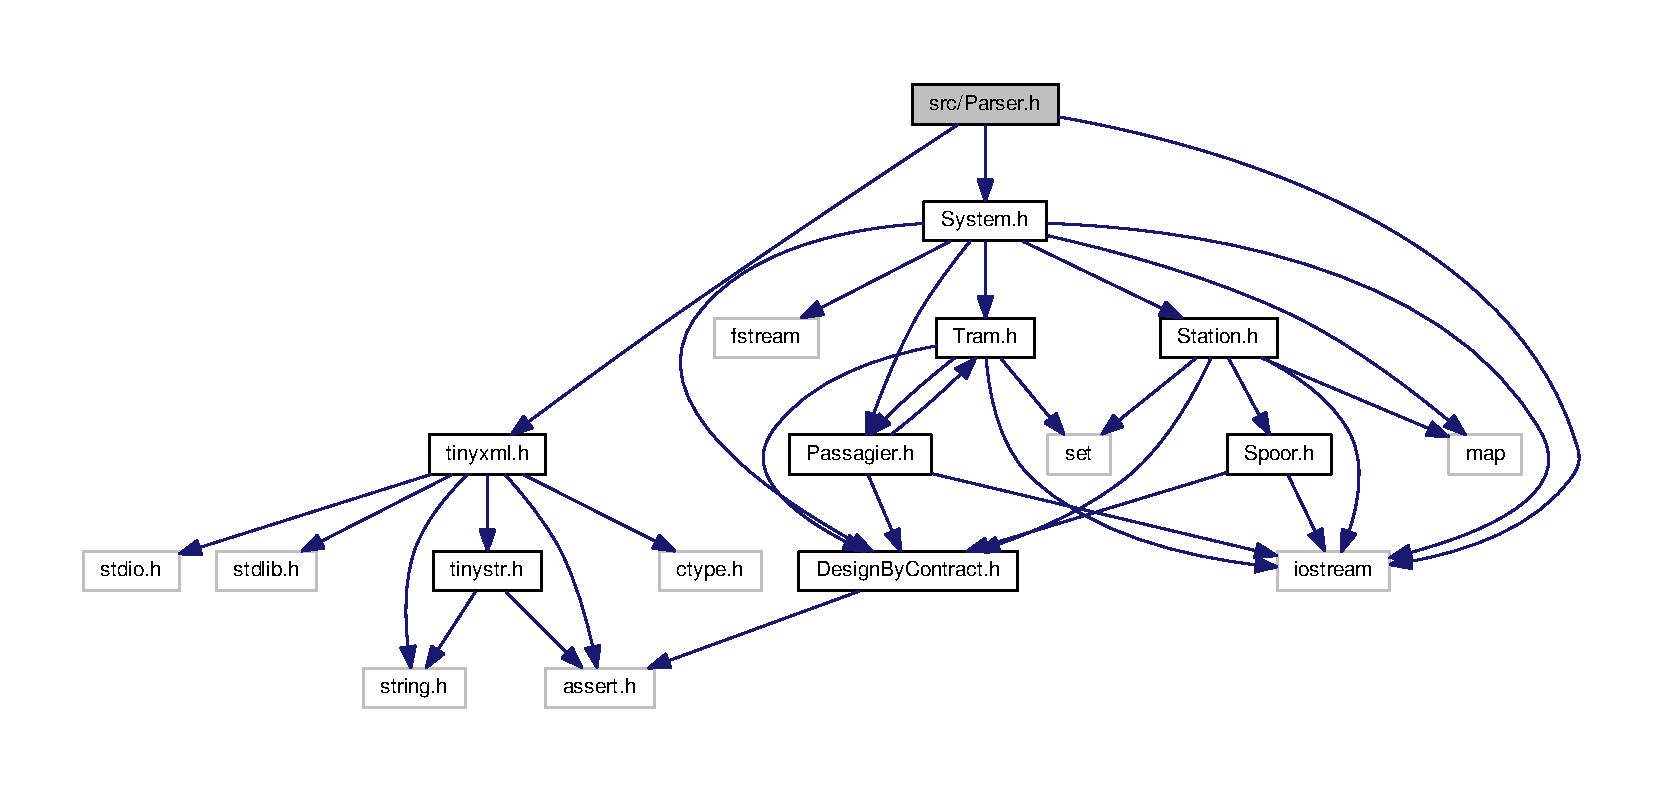
\includegraphics[width=350pt]{Parser_8h__incl}
\end{center}
\end{figure}
\subsection*{Classes}
\begin{DoxyCompactItemize}
\item 
class \hyperlink{classParser}{Parser}
\begin{DoxyCompactList}\small\item\em This Class contains all the functionalities for the \hyperlink{classParser}{Parser} objects. \end{DoxyCompactList}\end{DoxyCompactItemize}


\subsection{Detailed Description}
Header file for the \hyperlink{classParser}{Parser} Class. 


\hypertarget{Passagier_8h}{}\section{src/\+Passagier.h File Reference}
\label{Passagier_8h}\index{src/\+Passagier.\+h@{src/\+Passagier.\+h}}


Header file for the \hyperlink{classPassagier}{Passagier} Class.  


{\ttfamily \#include $<$iostream$>$}\\*
{\ttfamily \#include \char`\"{}Design\+By\+Contract.\+h\char`\"{}}\\*
{\ttfamily \#include \char`\"{}Tram.\+h\char`\"{}}\\*
Include dependency graph for Passagier.\+h\+:
\nopagebreak
\begin{figure}[H]
\begin{center}
\leavevmode
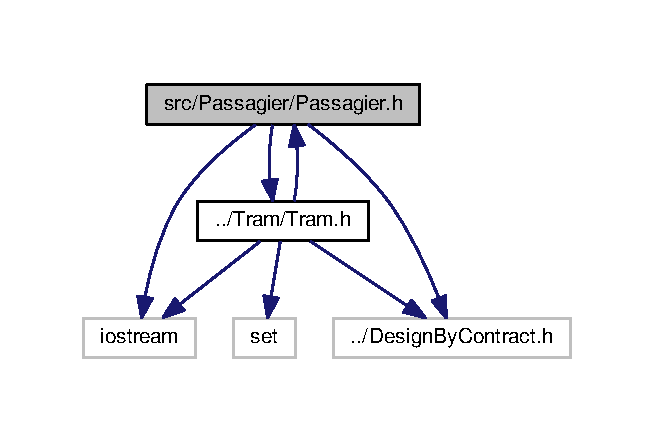
\includegraphics[width=306pt]{Passagier_8h__incl}
\end{center}
\end{figure}
This graph shows which files directly or indirectly include this file\+:
\nopagebreak
\begin{figure}[H]
\begin{center}
\leavevmode
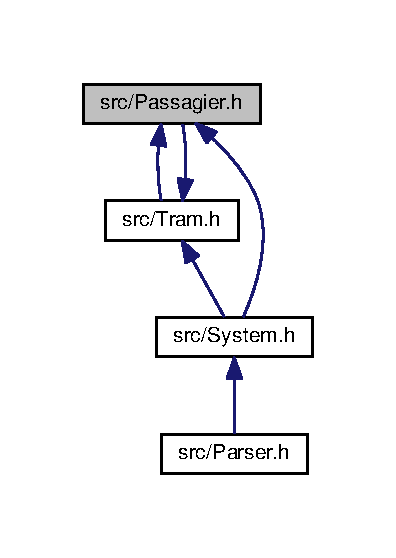
\includegraphics[width=165pt]{Passagier_8h__dep__incl}
\end{center}
\end{figure}
\subsection*{Classes}
\begin{DoxyCompactItemize}
\item 
class \hyperlink{classPassagier}{Passagier}
\begin{DoxyCompactList}\small\item\em This Class contains all the functionalities for the \hyperlink{classPassagier}{Passagier} objects. \end{DoxyCompactList}\end{DoxyCompactItemize}


\subsection{Detailed Description}
Header file for the \hyperlink{classPassagier}{Passagier} Class. 


\hypertarget{Spoor_8h}{}\section{src/\+Spoor/\+Spoor.h File Reference}
\label{Spoor_8h}\index{src/\+Spoor/\+Spoor.\+h@{src/\+Spoor/\+Spoor.\+h}}


Header file for the \hyperlink{classSpoor}{Spoor} Class.  


{\ttfamily \#include $<$iostream$>$}\\*
{\ttfamily \#include \char`\"{}../\+Design\+By\+Contract.\+h\char`\"{}}\\*
Include dependency graph for Spoor.\+h\+:\nopagebreak
\begin{figure}[H]
\begin{center}
\leavevmode
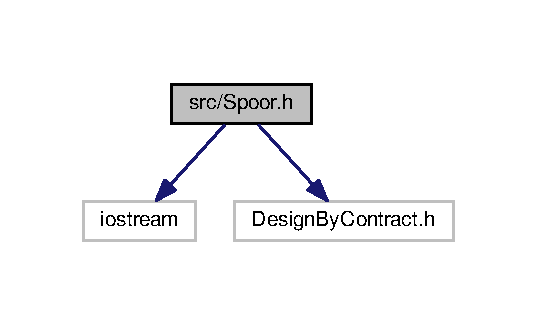
\includegraphics[width=266pt]{Spoor_8h__incl}
\end{center}
\end{figure}
This graph shows which files directly or indirectly include this file\+:\nopagebreak
\begin{figure}[H]
\begin{center}
\leavevmode
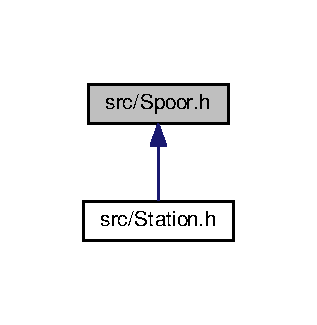
\includegraphics[width=350pt]{Spoor_8h__dep__incl}
\end{center}
\end{figure}
\subsection*{Classes}
\begin{DoxyCompactItemize}
\item 
class \hyperlink{classSpoor}{Spoor}
\begin{DoxyCompactList}\small\item\em This Class contains all the functionalities for the \hyperlink{classSpoor}{Spoor} objects. \end{DoxyCompactList}\end{DoxyCompactItemize}


\subsection{Detailed Description}
Header file for the \hyperlink{classSpoor}{Spoor} Class. 


\hypertarget{Halte_8h}{}\section{src/\+Station/\+Halte.h File Reference}
\label{Halte_8h}\index{src/\+Station/\+Halte.\+h@{src/\+Station/\+Halte.\+h}}


Header file for the \hyperlink{classHalte}{Halte} Class.  


{\ttfamily \#include \char`\"{}Station.\+h\char`\"{}}\\*
Include dependency graph for Halte.\+h\+:\nopagebreak
\begin{figure}[H]
\begin{center}
\leavevmode
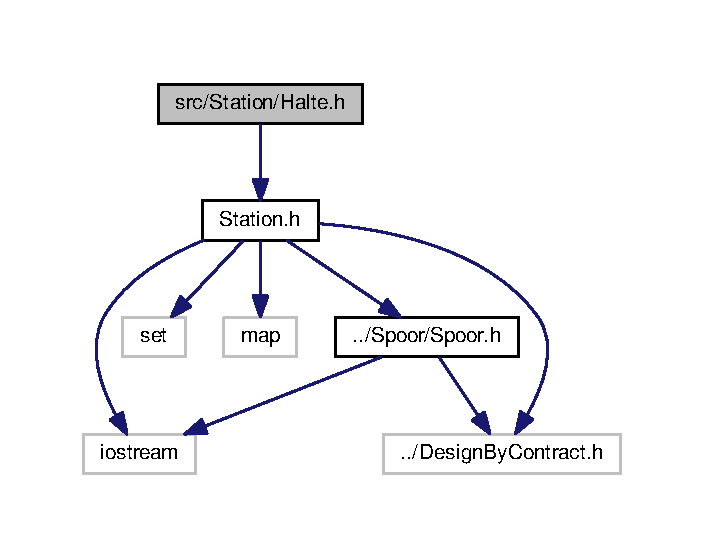
\includegraphics[width=338pt]{Halte_8h__incl}
\end{center}
\end{figure}
\subsection*{Classes}
\begin{DoxyCompactItemize}
\item 
class \hyperlink{classHalte}{Halte}
\begin{DoxyCompactList}\small\item\em This Class contains all the functionalities for the \hyperlink{classHalte}{Halte} objects, which is a derived class of the \hyperlink{classStation}{Station} class. \end{DoxyCompactList}\end{DoxyCompactItemize}


\subsection{Detailed Description}
Header file for the \hyperlink{classHalte}{Halte} Class. 


\hypertarget{Metrostation_8h}{}\section{src/\+Station/\+Metrostation.h File Reference}
\label{Metrostation_8h}\index{src/\+Station/\+Metrostation.\+h@{src/\+Station/\+Metrostation.\+h}}


Header file for the \hyperlink{classMetrostation}{Metrostation} Class.  


{\ttfamily \#include \char`\"{}Station.\+h\char`\"{}}\\*
Include dependency graph for Metrostation.\+h\+:\nopagebreak
\begin{figure}[H]
\begin{center}
\leavevmode
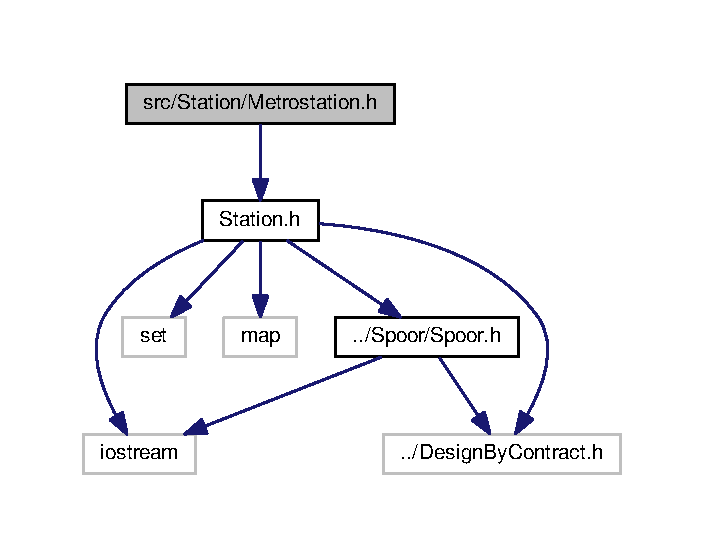
\includegraphics[width=338pt]{Metrostation_8h__incl}
\end{center}
\end{figure}
\subsection*{Classes}
\begin{DoxyCompactItemize}
\item 
class \hyperlink{classMetrostation}{Metrostation}
\begin{DoxyCompactList}\small\item\em This Class contains all the functionalities for the \hyperlink{classMetrostation}{Metrostation} objects, which is a derived class of the \hyperlink{classStation}{Station} class. \end{DoxyCompactList}\end{DoxyCompactItemize}


\subsection{Detailed Description}
Header file for the \hyperlink{classMetrostation}{Metrostation} Class. 


\hypertarget{Station_8h}{}\section{src/\+Station.h File Reference}
\label{Station_8h}\index{src/\+Station.\+h@{src/\+Station.\+h}}


Header file for the \hyperlink{classStation}{Station} Class.  


{\ttfamily \#include $<$iostream$>$}\\*
{\ttfamily \#include $<$set$>$}\\*
{\ttfamily \#include $<$map$>$}\\*
{\ttfamily \#include \char`\"{}Design\+By\+Contract.\+h\char`\"{}}\\*
{\ttfamily \#include \char`\"{}Spoor.\+h\char`\"{}}\\*
Include dependency graph for Station.\+h\+:\nopagebreak
\begin{figure}[H]
\begin{center}
\leavevmode
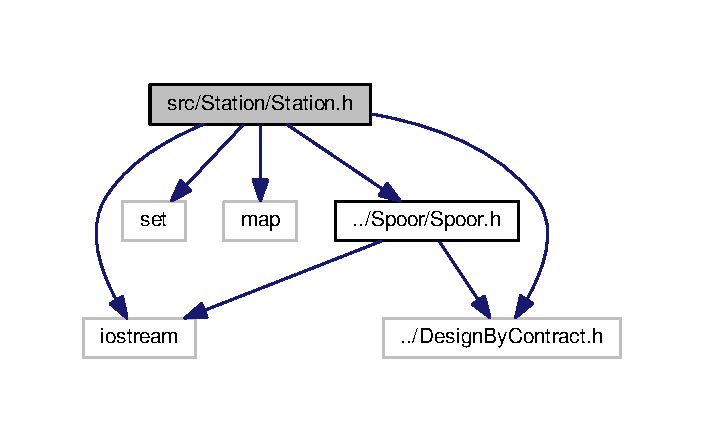
\includegraphics[width=313pt]{Station_8h__incl}
\end{center}
\end{figure}
This graph shows which files directly or indirectly include this file\+:\nopagebreak
\begin{figure}[H]
\begin{center}
\leavevmode
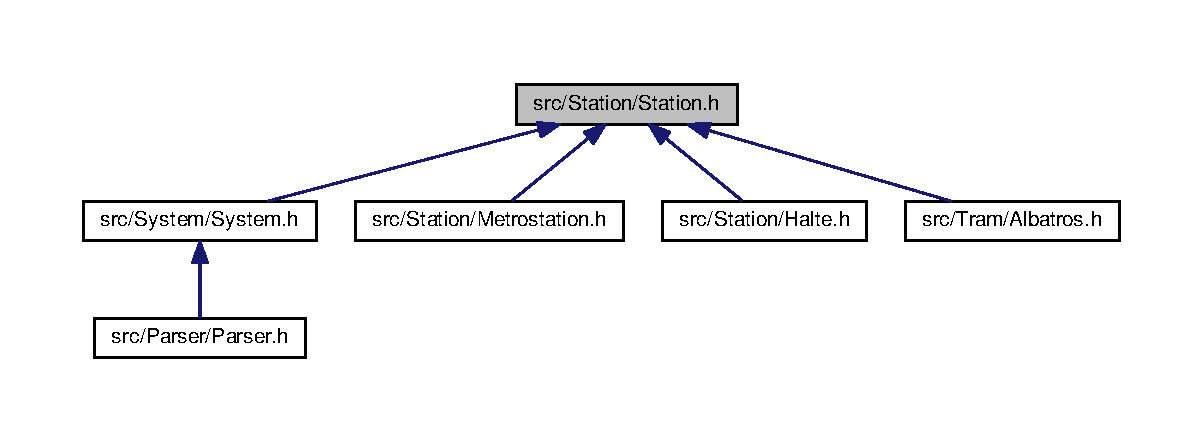
\includegraphics[width=155pt]{Station_8h__dep__incl}
\end{center}
\end{figure}
\subsection*{Classes}
\begin{DoxyCompactItemize}
\item 
class \hyperlink{classStation}{Station}
\begin{DoxyCompactList}\small\item\em This Class contains all the functionalities for the \hyperlink{classStation}{Station} objects. \end{DoxyCompactList}\end{DoxyCompactItemize}


\subsection{Detailed Description}
Header file for the \hyperlink{classStation}{Station} Class. 


\hypertarget{System_8h}{}\section{src/\+System/\+System.h File Reference}
\label{System_8h}\index{src/\+System/\+System.\+h@{src/\+System/\+System.\+h}}


Header file for \hyperlink{classSystem}{System} class.  


{\ttfamily \#include \char`\"{}../\+Station/\+Station.\+h\char`\"{}}\\*
{\ttfamily \#include \char`\"{}../\+Tram/\+Tram.\+h\char`\"{}}\\*
{\ttfamily \#include \char`\"{}../\+Passagier/\+Passagier.\+h\char`\"{}}\\*
{\ttfamily \#include $<$iostream$>$}\\*
{\ttfamily \#include $<$map$>$}\\*
{\ttfamily \#include $<$fstream$>$}\\*
{\ttfamily \#include \char`\"{}../\+Design\+By\+Contract.\+h\char`\"{}}\\*
Include dependency graph for System.\+h\+:\nopagebreak
\begin{figure}[H]
\begin{center}
\leavevmode
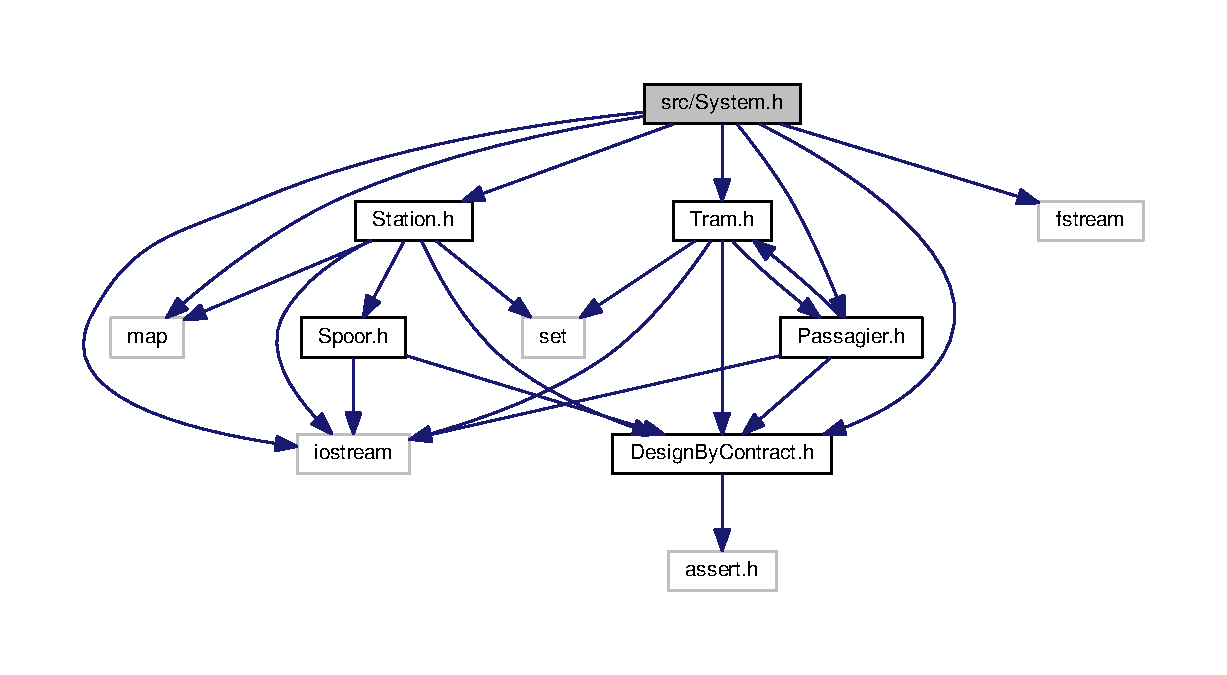
\includegraphics[width=350pt]{System_8h__incl}
\end{center}
\end{figure}
This graph shows which files directly or indirectly include this file\+:\nopagebreak
\begin{figure}[H]
\begin{center}
\leavevmode
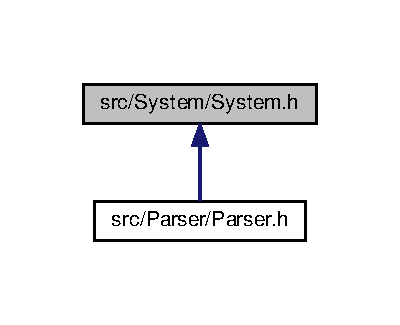
\includegraphics[width=192pt]{System_8h__dep__incl}
\end{center}
\end{figure}
\subsection*{Classes}
\begin{DoxyCompactItemize}
\item 
class \hyperlink{classSystem}{System}
\begin{DoxyCompactList}\small\item\em This Class contains all the functionalities for the \hyperlink{classSystem}{System} objects. \end{DoxyCompactList}\end{DoxyCompactItemize}


\subsection{Detailed Description}
Header file for \hyperlink{classSystem}{System} class. 


\hypertarget{Albatros_8h}{}\section{src/\+Tram/\+Albatros.h File Reference}
\label{Albatros_8h}\index{src/\+Tram/\+Albatros.\+h@{src/\+Tram/\+Albatros.\+h}}


Header file for the \hyperlink{classAlbatros}{Albatros} Class.  


{\ttfamily \#include \char`\"{}Tram.\+h\char`\"{}}\\*
{\ttfamily \#include \char`\"{}../\+Station/\+Station.\+h\char`\"{}}\\*
Include dependency graph for Albatros.\+h\+:\nopagebreak
\begin{figure}[H]
\begin{center}
\leavevmode
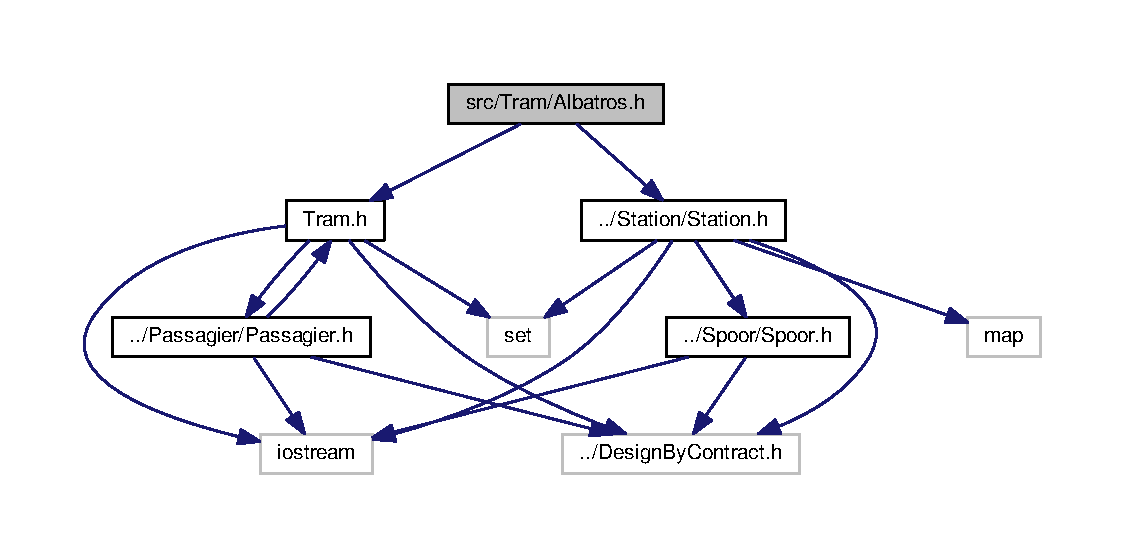
\includegraphics[width=350pt]{Albatros_8h__incl}
\end{center}
\end{figure}
\subsection*{Classes}
\begin{DoxyCompactItemize}
\item 
class \hyperlink{classAlbatros}{Albatros}
\begin{DoxyCompactList}\small\item\em This Class contains all the functionalities for the \hyperlink{classAlbatros}{Albatros} objects, which is a derived class of the \hyperlink{classTram}{Tram} class. \end{DoxyCompactList}\end{DoxyCompactItemize}


\subsection{Detailed Description}
Header file for the \hyperlink{classAlbatros}{Albatros} Class. 


\hypertarget{Tram_8h}{}\section{src/\+Tram.h File Reference}
\label{Tram_8h}\index{src/\+Tram.\+h@{src/\+Tram.\+h}}


Header file for the \hyperlink{classTram}{Tram} Class.  


{\ttfamily \#include $<$iostream$>$}\\*
{\ttfamily \#include $<$set$>$}\\*
{\ttfamily \#include \char`\"{}Design\+By\+Contract.\+h\char`\"{}}\\*
{\ttfamily \#include \char`\"{}Passagier.\+h\char`\"{}}\\*
Include dependency graph for Tram.\+h\+:
\nopagebreak
\begin{figure}[H]
\begin{center}
\leavevmode
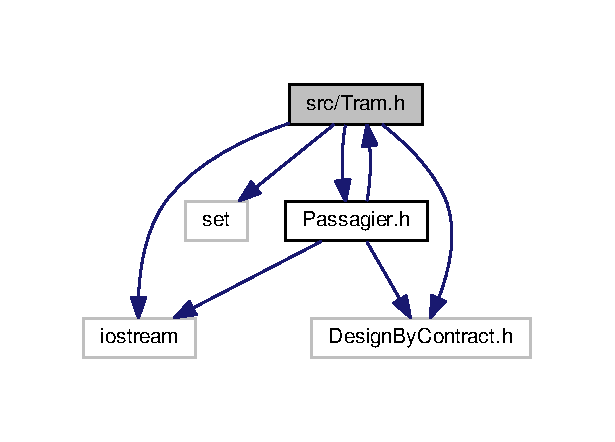
\includegraphics[width=295pt]{Tram_8h__incl}
\end{center}
\end{figure}
This graph shows which files directly or indirectly include this file\+:
\nopagebreak
\begin{figure}[H]
\begin{center}
\leavevmode
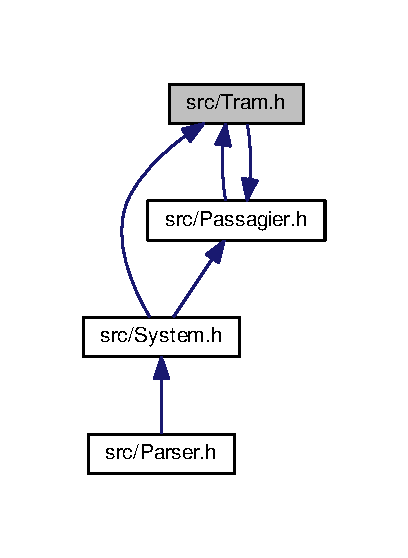
\includegraphics[width=196pt]{Tram_8h__dep__incl}
\end{center}
\end{figure}
\subsection*{Classes}
\begin{DoxyCompactItemize}
\item 
class \hyperlink{classTram}{Tram}
\begin{DoxyCompactList}\small\item\em This Class contains all the functionalities for the \hyperlink{classTram}{Tram} objects. \end{DoxyCompactList}\end{DoxyCompactItemize}


\subsection{Detailed Description}
Header file for the \hyperlink{classTram}{Tram} Class. 


%--- End generated contents ---

% Index
\backmatter
\newpage
\phantomsection
\clearemptydoublepage
\addcontentsline{toc}{chapter}{Index}
\printindex

\end{document}
